\documentclass[a4paper,12pt]{article} % добавить leqno в [] для нумерации слева
% \usepackage[a4paper,top=1.3cm,bottom=2cm,left=1.5cm,right=1.5cm,marginparwidth=0.75cm]{geometry}
\usepackage[left=1.5cm,right=1.5cm,top=2cm,bottom=2cm]{geometry}
%%% Работа с русским языком
\usepackage{cmap}					% поиск в PDF
\usepackage{mathtext} 				% русские буквы в формулах
\usepackage[T2A]{fontenc}			% кодировка
\usepackage[utf8]{inputenc}			% кодировка исходного текста
\usepackage[english,russian]{babel}	% локализация и переносы


%%% Работа с русским языком
\usepackage{cmap}                           % поиск в PDF
\usepackage{mathtext} 			 	       % русские буквы в формулах
\usepackage[T2A]{fontenc}               % кодировка
\usepackage[utf8]{inputenc}              % кодировка исходного текста
\usepackage[english,russian]{babel}  % локализация и переносы

\usepackage{graphicx}
\graphicspath{{noiseimages/}}
\usepackage{wrapfig}
\usepackage{tabularx}
\usepackage{hyphenat}
\usepackage{hyperref}
\usepackage{gensymb}
\usepackage[rgb]{xcolor}
\hypersetup{
colorlinks=true,urlcolor=blue
}


%%% Дополнительная работа с математикой
\usepackage{amsmath,amsfonts,amssymb,amsthm,mathtools} % AMS
\usepackage{icomma} % "Умная" запятая: $0,2$ --- число, $0, 2$ --- перечисление

%% Номера формул
%\mathtoolsset{showonlyrefs=true} % Показывать номера только у тех формул, на которые есть \eqref{} в тексте.

%% Шрифты
\usepackage{euscript}	 % Шрифт Евклид
\usepackage{mathrsfs} % Красивый матшрифт

%% Свои команды
\DeclareMathOperator{\sgn}{\mathop{sgn}}

%% Перенос знаков в формулах (по Львовскому)
\newcommand*{\hm}[1]{#1\nobreak\discretionary{}
{\hbox{$\mathsurround=0pt #1$}}{}}




\date{\today}

\begin{document}

\begin{titlepage}
	\begin{center}
		{\large МОСКОВСКИЙ ФИЗИКО-ТЕХНИЧЕСКИЙ ИНСТИТУТ (НАЦИОНАЛЬНЫЙ ИССЛЕДОВАТЕЛЬСКИЙ УНИВЕРСИТЕТ)}
	\end{center}
    \begin{center}
		{\large Физтех-школа аэрокосмических технологий}
	\end{center}


	\vspace{4.5cm}
	{\huge
		\begin{center}
			{\bf Отчёт о выполнении лабораторной работы 3.6.1}\\
		Спектральный анализ электр. сигналов
		\end{center}
	}
	\vspace{2cm}
	\begin{flushright}
		{\LARGE Авторы:\\Болдинский Дмитрий Олегович\\
            \vspace{0.1cm}
        Байкова Алина Алексеевна\\
       
			\vspace{1cm}
			Группа Б03-201}
	\end{flushright}

\vspace{2cm}
 
\begin{center}
\includegraphics[width=0.2\linewidth]{fakt.png}
\end{center}

 
	\vspace{0.5cm}
	\begin{center}
		Долгопрудный, 2023
	\end{center}
\end{titlepage}



\section{Аннотация}
\indent
\indent \textbf{Цель работы:} изучить спектры сигналов различной формы и влияние параметров сигнала
на вид соответствующих спектров; проверить справедливость соотношений неопределённостей; познакомиться с работой спектральных фильтров на примере RC-цепочки

\indent \textbf{В работе используются:} генератор сигналов произвольной формы, цифровой осциллограф с функцией быстрого преобразования Фурье или цифровой USB-осциллограф, подключённый к персональному компьютеру.





\section{Теоретическое введение}

\subsection*{Разложение сложных сигналов на периодические колебания}
Представление периодического сигнала в виде суммы гармонических сигналов называется разложением в ряд Фурье.
	
	Пусть заданная функция $f(t)$ периодически повторяется с частотой $\Omega_{1}=\dfrac{2\pi}{T},$ где $T$ - период повторения. Ее разложение в ряд Фурье имеет вид
\begin{equation}
    f(t)=\dfrac{a_{0}}{2}+ \sum\limits_{n=1}^\infty [a_{n}\cos(n \Omega_{1}t)+b_{n}\sin(n \Omega_{1} t) ]
\label{eq1}
\end{equation}
		Здесь $\dfrac{a_{0}}{2}$ - среднее значение функции $f(t)$,
	
\begin{equation}
     a_{n}=\dfrac{2}{T}\int\limits_{t_{1}}^{t_{1}+T}f(t)\cos(n \Omega_{1} t)dt, 
     \label{eq2}
\end{equation}
\begin{equation}
    b_{n}=\dfrac{2}{T}\int\limits_{t_{1}}^{t_{1}+T}f(t)\sin(n \Omega_{1} t)dt.
    \label{eq3}
\end{equation}
  

	
	
	Рассмотрим периодические функции, которые исследуются в нашей
	работе.
	
	\begin{enumerate}
		
	\item 	\textbf{Периодическая последовательность прямоугольных импульсов} (рис. 1) с амплитудой $V_{0}$, длительностью $\tau$, частотой повторения $\Omega_{1}=\dfrac{2\pi}{T},$ где $T$ - период повторения импульсов. Найдем коэффициенты разложения ряда Фурье:
	
	$$\dfrac{a_{0}}{2}=V_{0}\dfrac{\tau}{T},$$

 \begin{equation}
     a_{n}=\dfrac{2}{T}\int\limits_{-\frac{\tau}{2}}^{\frac{\tau}{2}}V_{0}\cos(n \Omega_{1} t)dt=2V_{0}\dfrac{\tau}{T}\dfrac{\sin(n \Omega_{1} \frac{\tau}{2})}{n\Omega_{1}\frac{\tau}{2}} \sim \dfrac{\sin x}{x}.
    \label{eq4}
 \end{equation}

	
	Поскольку наша функция четная, все коэффициенты синусоидальных гармоник $b_{n}=0$. Спектр $a_{n}$ последовательности прямоугольных импульсов представлен на рис. 2 (изображен случай, когда $T$ кратно $\tau$).
		
		
		\begin{figure}[h]
			\begin{minipage}[h]{0.5\linewidth}
				\center{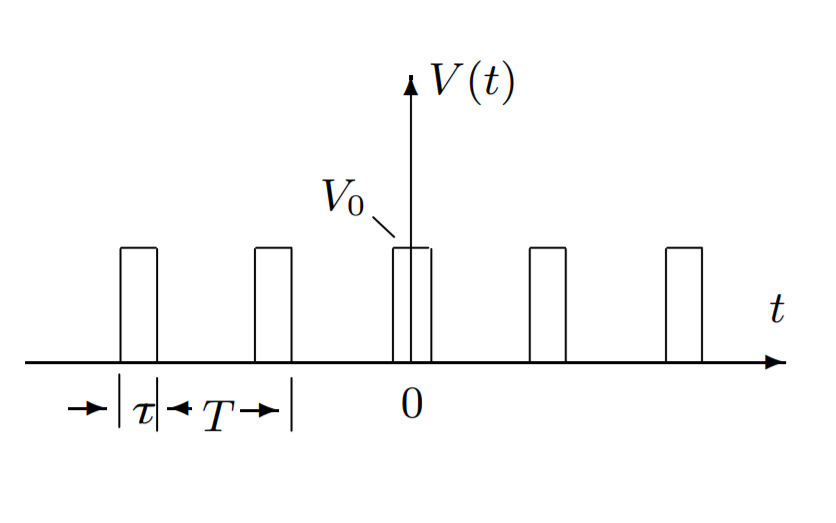
\includegraphics[width=0.9\linewidth]{sp1.png}}
				\caption{Прямоугольные импульсы}
			\end{minipage}
			\begin{minipage}[h]{0.5\linewidth}
				\center{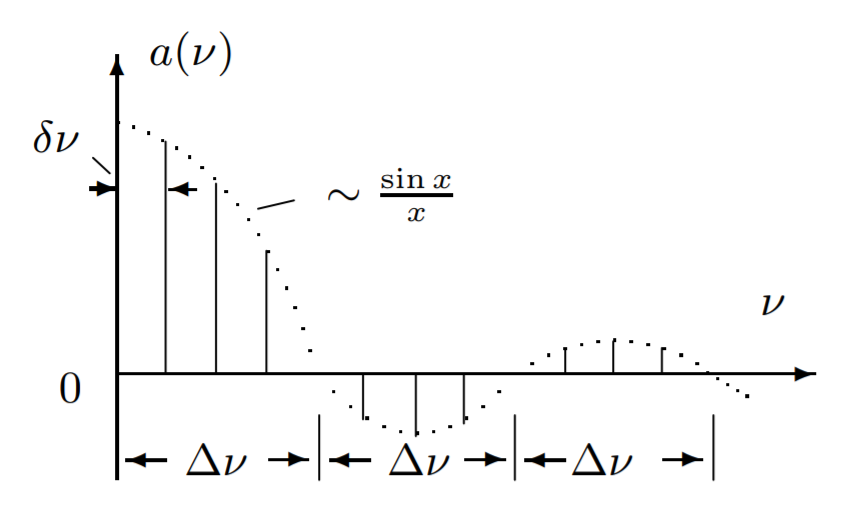
\includegraphics[width=0.9\linewidth]{sp2.png}}
				\caption{Спектр последовательности прямоугольных импульсов}
			\end{minipage}
		\end{figure}
	
	Назовем \textit{шириной спектра} $\Delta \omega$ расстояние от главного максимума ($\omega =0$) до первого нуля огибающей, возникающего при $n=\dfrac{2\pi}{\tau \Omega_{1}}$. При этом 

	$$\Delta \omega \tau \backsimeq 2 \pi $$
	
	 или 
	
\begin{equation}\label{neopr}
	\Delta \nu \Delta t \backsimeq 1
\label{eq5}
\end{equation}
		
	Полученное соотношение взаимной связи интервалов $\Delta \nu$ и $\Delta t$ является
	частным случаем соотношения неопределенности в квантовой механике.
	
	\item \textbf{Периодическая последовательность цугов} гармонического колебания $V_{0}\cos(\omega_{0}t)$ с длительностью цуга $\tau$ и периодом повторения $T$ (рис. 3).
	
	Функция $f(t)$ снова является четной относительно $t=0$. Коэффициент при $n$-й гармонике равен
\begin{equation}
    a_{n}=\dfrac{2}{T}\int\limits_{-\frac{\tau}{2}}^{\frac{\tau}{2}}V_{0}\cos(\omega_{0}t)\cos(n \Omega_{1} t)dt=V_{0}\dfrac{\tau}{T} \bigg(\dfrac{\sin[(\omega_{0}-n\Omega_{1})\frac{\tau}{2}]}{(\omega_{0}-n\Omega_{1})\frac{\tau}{2}}+\dfrac{\sin[(\omega_{0}+n\Omega_{1})\frac{\tau}{2}]}{(\omega_{0}+n\Omega_{1})\frac{\tau}{2}} \bigg)
\label{eq6}
\end{equation}
	
	Зависимость для случая, когда $\frac{T}{\tau}$ равно целому числу, представлена на рис. 4. Сравнивая спектр последовательности прямоугольных импульсов и цугов мы видим, что они аналогичны, но их максимумы сдвинуты по частоте на величину $\omega_{0}$.
	
	\begin{figure}[h]
		\begin{minipage}[h]{0.5\linewidth}
			\center{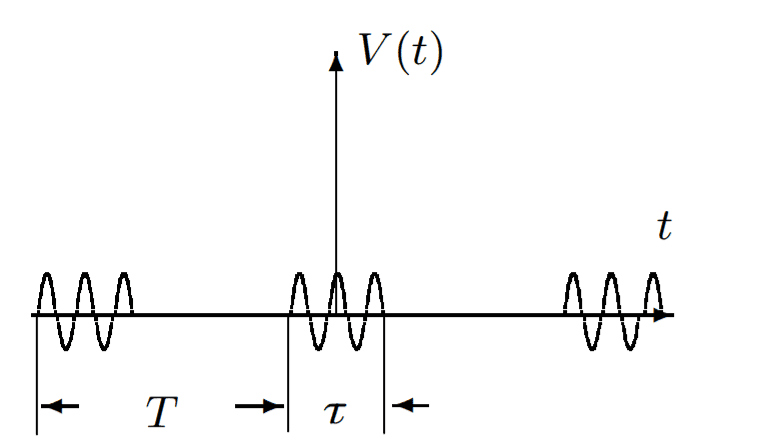
\includegraphics[width=0.9\linewidth]{sp3.png}}
			\caption{Последовательность цугов}
		\end{minipage}
		\begin{minipage}[h]{0.5\linewidth}
			\center{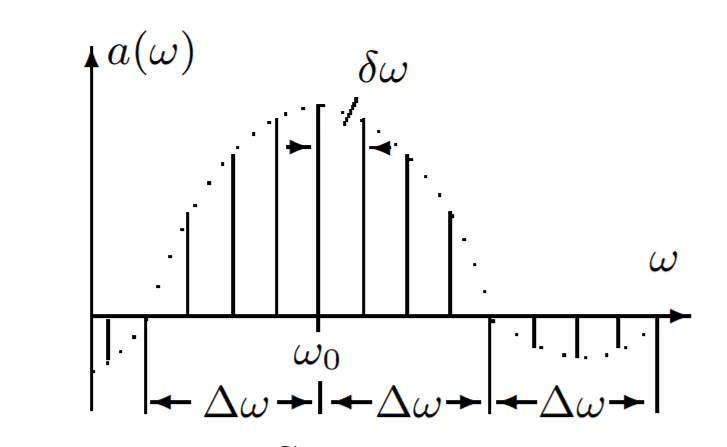
\includegraphics[width=0.9\linewidth]{sp4.png}}
			\caption{Спектр последовательности цугов}
		\end{minipage}
	\end{figure}

	\item \textbf{Амплитудно-модулированные колебания.} Рассмотрим гармонические колебания высокой частоты $\omega_{0}$ , амплитуда которых медленно меняется по гармоническому закону с частотой $\Omega$ ($\Omega \ll \omega_{0})$) (рис. 5):
\begin{equation}
    f(t)=A_{0}[1+m\cos\Omega t]\cos \omega_{0}t
\label{eq7}
\end{equation}	

	Коэффициент $m$ называют \textbf{глубиной модуляции}. При $m<1$ амплитуда колебаний меняется от минимальной $A_{min}=A_{0}(1-m)$ до максимальной $A_{max}=A_{0}(1+m).$ Глубина модуляции может быть представлена в виде
	
\begin{equation}\label{m}
	 m=\dfrac{A_{max}-A_{min}}{A_{max}+A_{min}}
\label{eq8}
\end{equation}
	
	Простым тригонометрическим преобразованием можно найти спектр амплитудно - модулированных колебаний:
	\\
\begin{equation}\label{a}
	f(t)=A_{0}\cos(\omega_{0} t)+\dfrac{A_{0}m}{2}\cos(\omega_{0}+\Omega)t+\dfrac{A_{0}m}{2}\cos(\omega_{0}-\Omega)t.
\end{equation}
		
		\begin{figure}[h]
			\begin{minipage}[h]{0.5\linewidth}
				\center{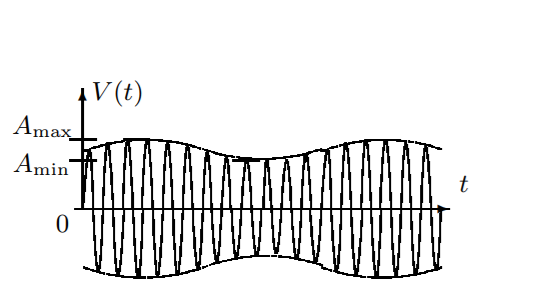
\includegraphics[width=0.9\linewidth]{sp5.png}}
				\caption{Модулированные гармонические колебания}
			\end{minipage}
			\begin{minipage}[h]{0.5\linewidth}
				\center{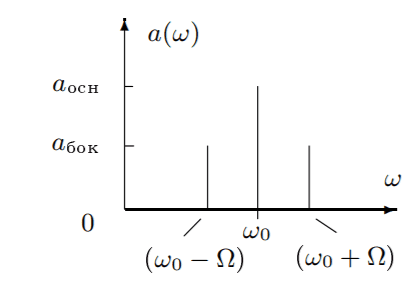
\includegraphics[width=0.9\linewidth]{sp6.png}}
				\caption{Спектр модулированных гармонических колебаний}
			\end{minipage}
		\end{figure}
		
		Спектр таких колебаний содержит три составляющих  основную
		компоненту и две боковых (рис. 6). Первое слагаемое в правой части представляет собой исходное немодулированное колебание
		с основной (несущей) частотой $\omega_{0}$ и амплитудой $a_{осн} = A_{0}$ . Второе и третье слагаемые соответствуют новым гармоническим колебаниям с частотами $\omega_{0} + \Omega$ и $\omega_{0} - \Omega$. Амплитуды этих двух колебаний одинаковы и составляют $\dfrac{m}{2}$ от амплитуды немодулированного колебания:
		$a_{бок} = \dfrac{A_{0}m}{2}$. Начальные фазы всех трех колебаний одинаковы.
	\end{enumerate}

\newpage

\section{Экспериментальная установка.}
В работе изучаются спектры периодических электрических сигналов 
различной формы (последовательности прямоугольных импульсов и цугов, 
а также амплитудно- и фазо-модулированных гармонических колебаний). 
Спектры этих сигналов наблюдаются с помощью спектроанализатора, входящего в состав USB-осциллографа и сравниваются с рассчитанными теоретически. Схема установки изображена на рис.\ref{ustanovka}
\begin{figure}[h]
    \centering
    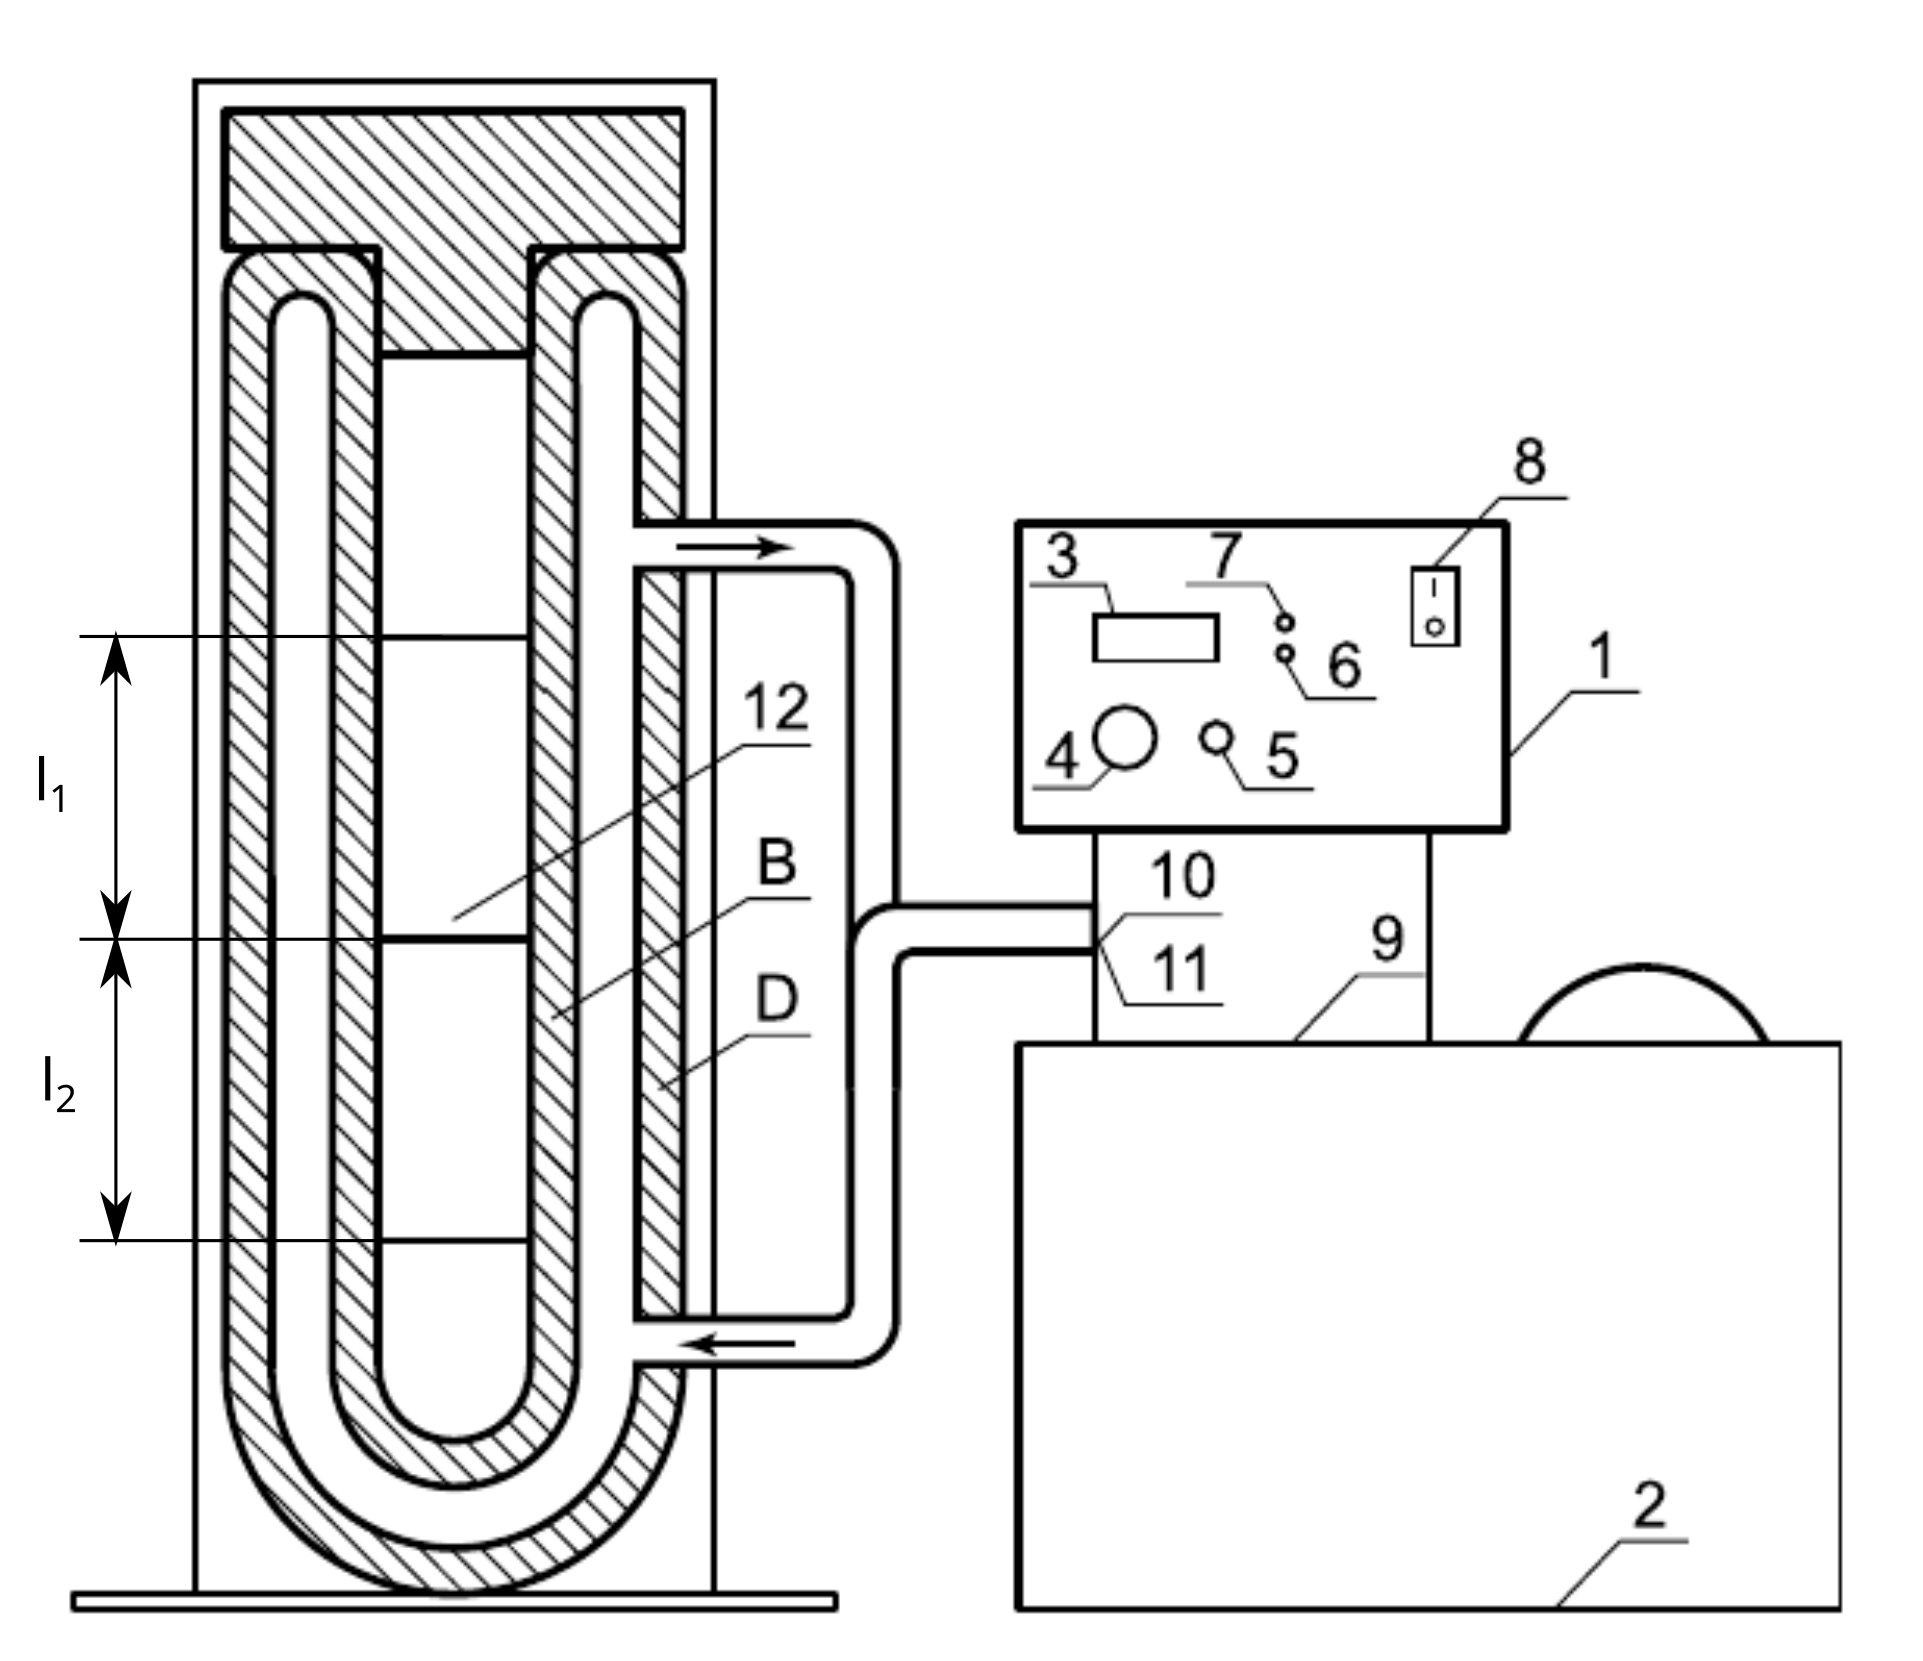
\includegraphics{ustanovka.png}
    \caption{Схема экспериментальной установки}
    \label{ustanovka}
\end{figure}

Функциональный генератор WaveStation 2012 позволяет сформировать два 
различных электрических сигнала, которые выводятся на два независимых канала – "CH1" и "CH2". Сигнал с канала "CH1" подается на вход "А", а сигнал с канала "CH2" – на вход "В" USB-осциллографа. Затем эти сигналы подаются на вход компьютера через USB-соединение. При работе USB-осциллографа в режиме осциллографа, на экране компьютера можно наблюдать каждый из сигналов в отдельности, а также их произведение. В режиме спектроанализатора можно наблюдать спектры этих сигналов.
При включении функционального генератора, на его экране отображается информация о параметрах электрического сигнала. На рис.\ref{generator1} показаны области на экране генератора, в которых отображены следующие 
данные:
А – форма или тип сигнала и номер выходного канала;
Б – форма и параметры выходного сигнала;
В – область установки параметров выходного сигнала;
Г – форма или тип сигнала;
Д – экранное меню для установки параметров сигнала.
\begin{figure}[h]
    \centering
    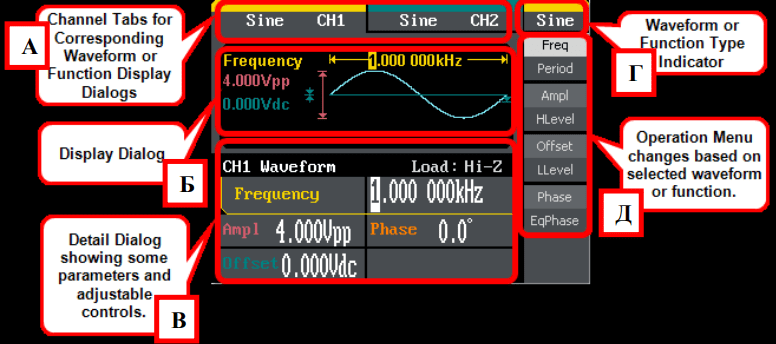
\includegraphics[width=0.8\linewidth]{generator1.png}
    \caption{Экран генератора}
    \label{generator1}
\end{figure}

Передняя панель функционального генератора показана на рис.\ref{generator2}.
1 – кнопка включения; 2 – USB-разъем; 3 – экран; 4 – кнопки экранного меню; 5 – кнопки выбора типа сигналов; 6 – цифровая панель; 7 - функциональные кнопки; 8 – разъемы с кнопками включения (выключения) выходных сигналов 1-го и 2-го каналов; 9 – кнопки перемещения; 10 – подстроечный регулятор.
\begin{figure}[h]
    \centering
    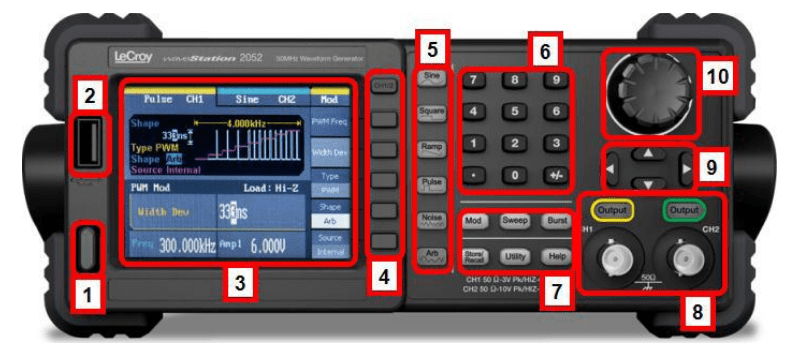
\includegraphics[width=0.9\linewidth]{generator2.png}
    \caption{Передняя панель функционального генератора}
    \label{generator2}
\end{figure}


\newpage
\section{Ход работы}

\subsection*{А. Исследование спектра периодической последовательности
прямоугольных импульсов и проверка соотношений неопределённости}

\begin{enumerate}

\item [\textbf{1.}]  Настраиваем генератор на прямоугольные импульсы с частотой повторения $\nu_\text{повт}$ = 1 кГц (период $T$ = 1 мс) и
длительностью импульса $\tau$ = $T$/20 = 50 мкс.

\item [\textbf{2.}] Получаем на экране спектр (Преобразование Фурье) сигнала.

\textbf{a.} Изменяем $\nu_\text{повт}$ при фиксированном $\tau$ = 50 мкс и получаем:

\begin{figure}[h]
\begin{minipage}[h]{0.47\linewidth}
\center{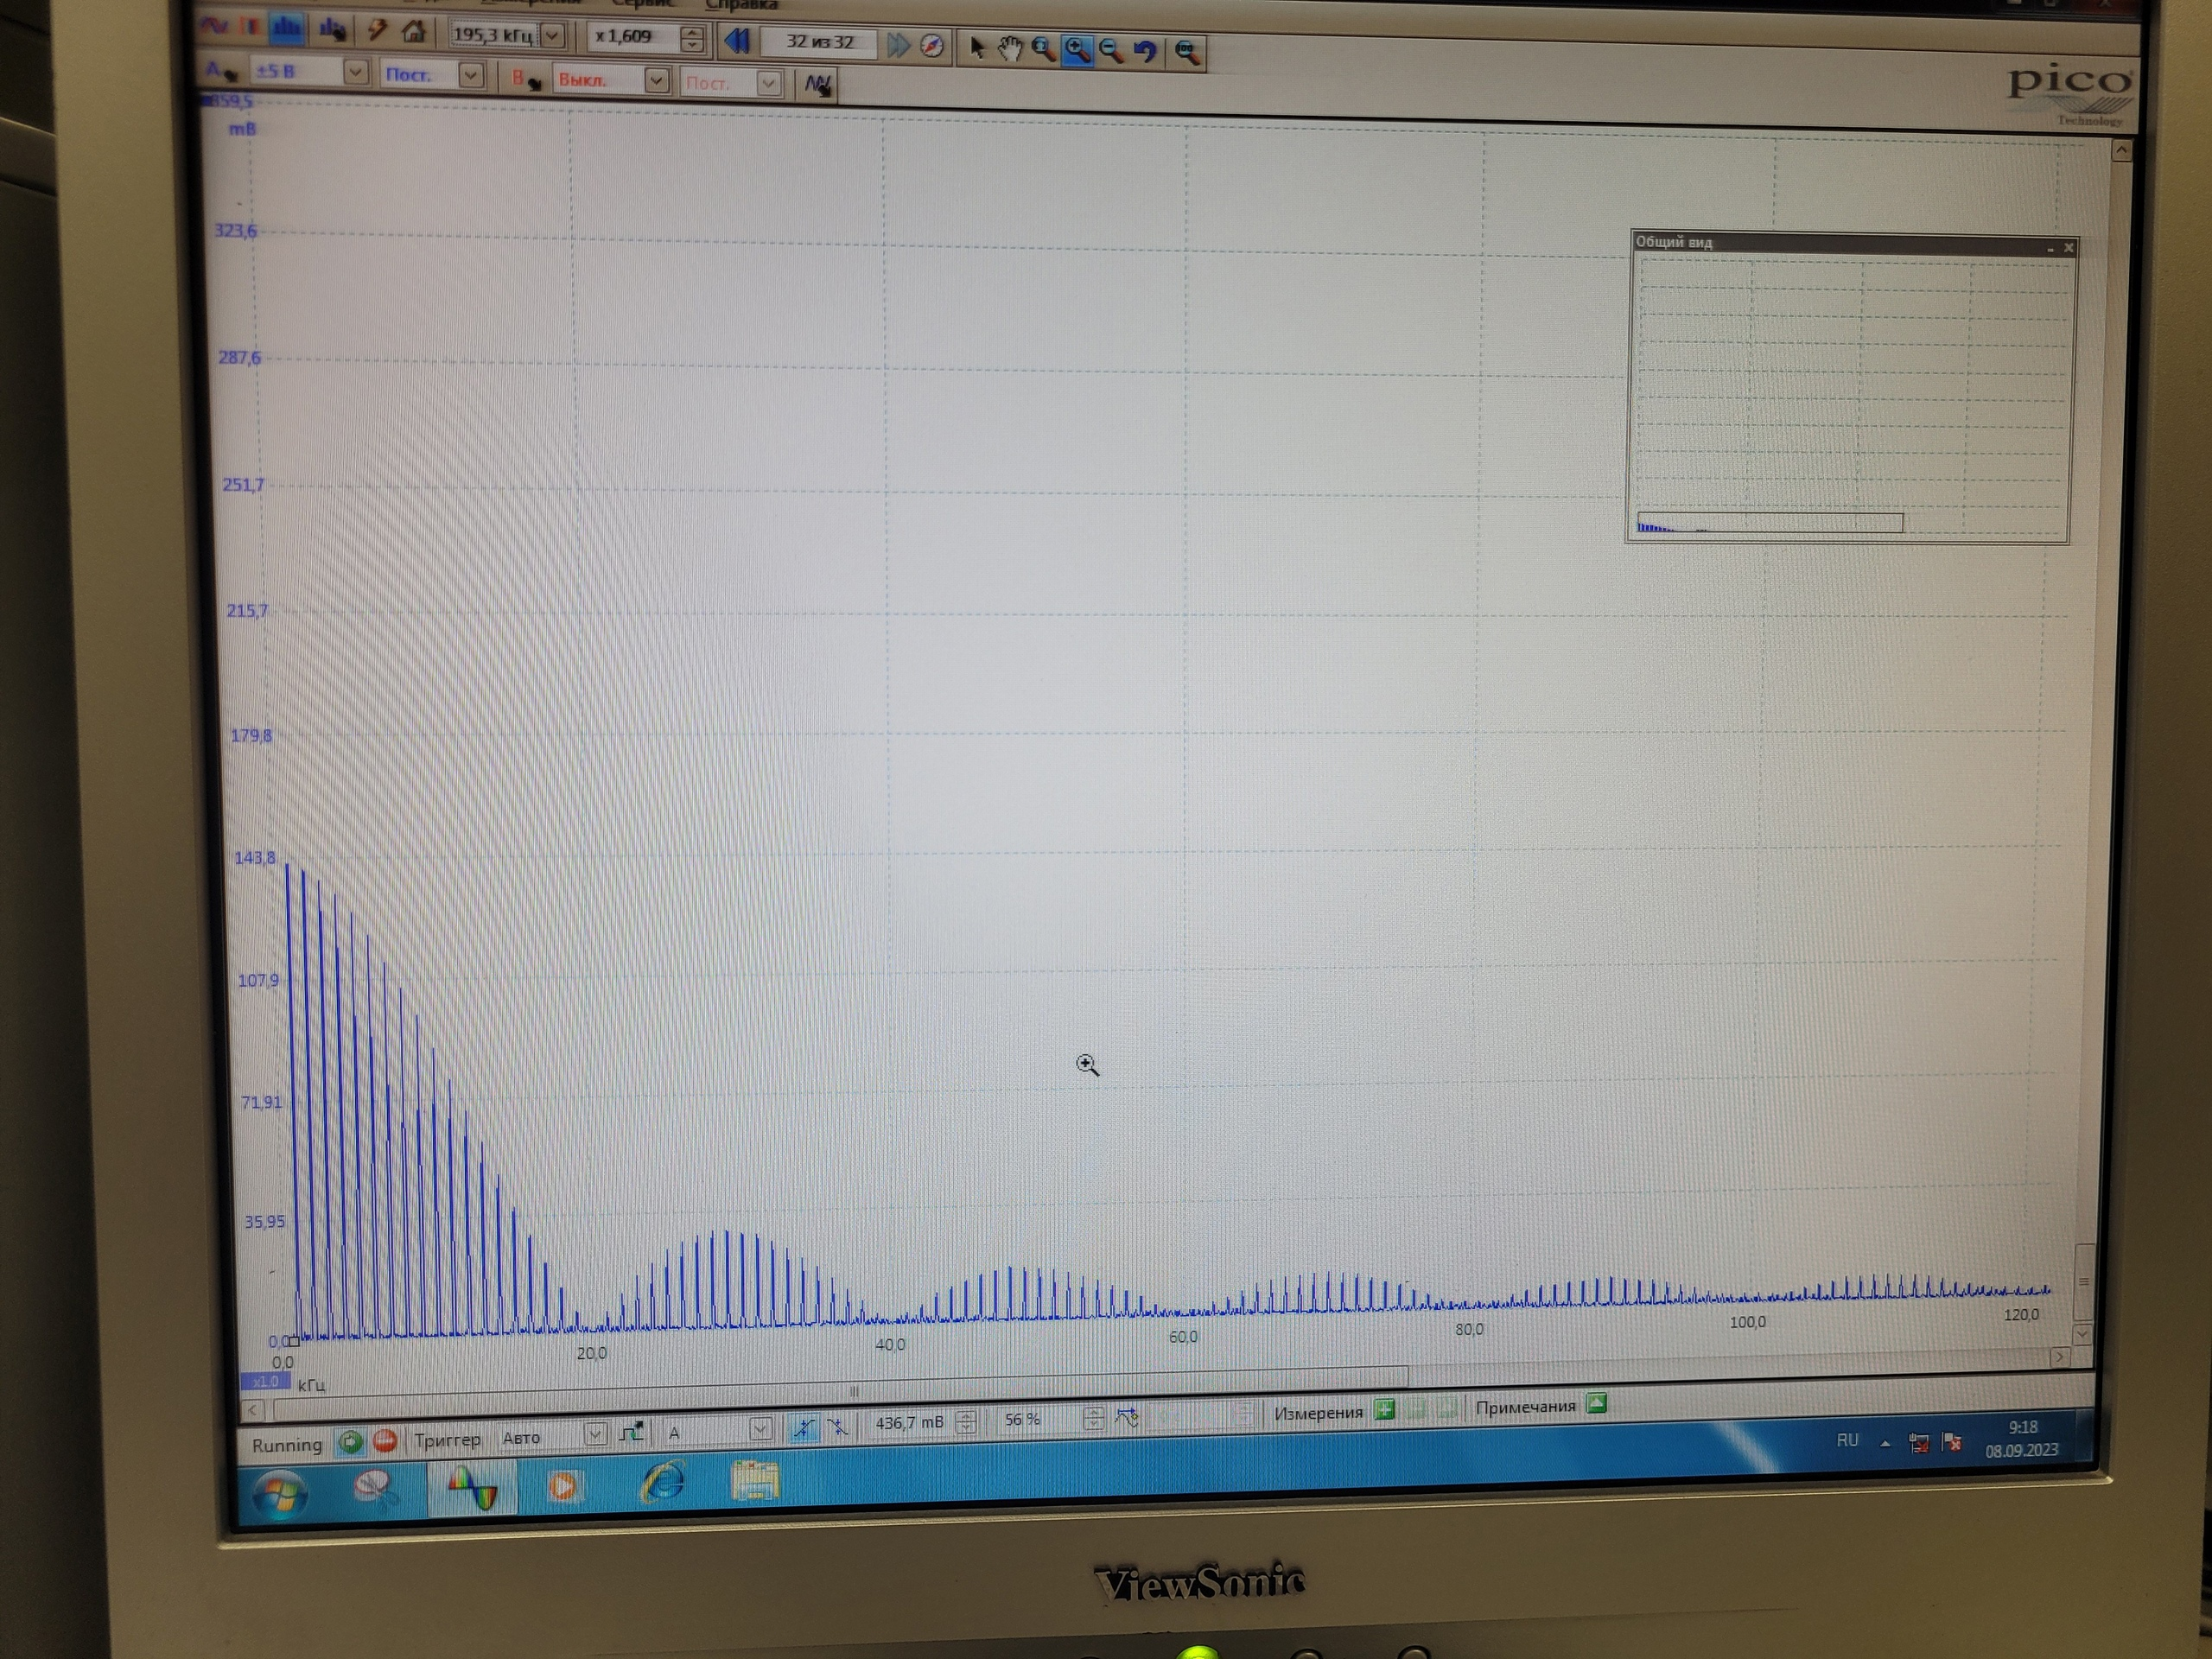
\includegraphics[width=1\linewidth]{A_1k_50.jpg}}  \\$\nu_\text{повт}$ = 1 кГц 
\end{minipage}
\hfill
\begin{minipage}[h]{0.47\linewidth}
\center{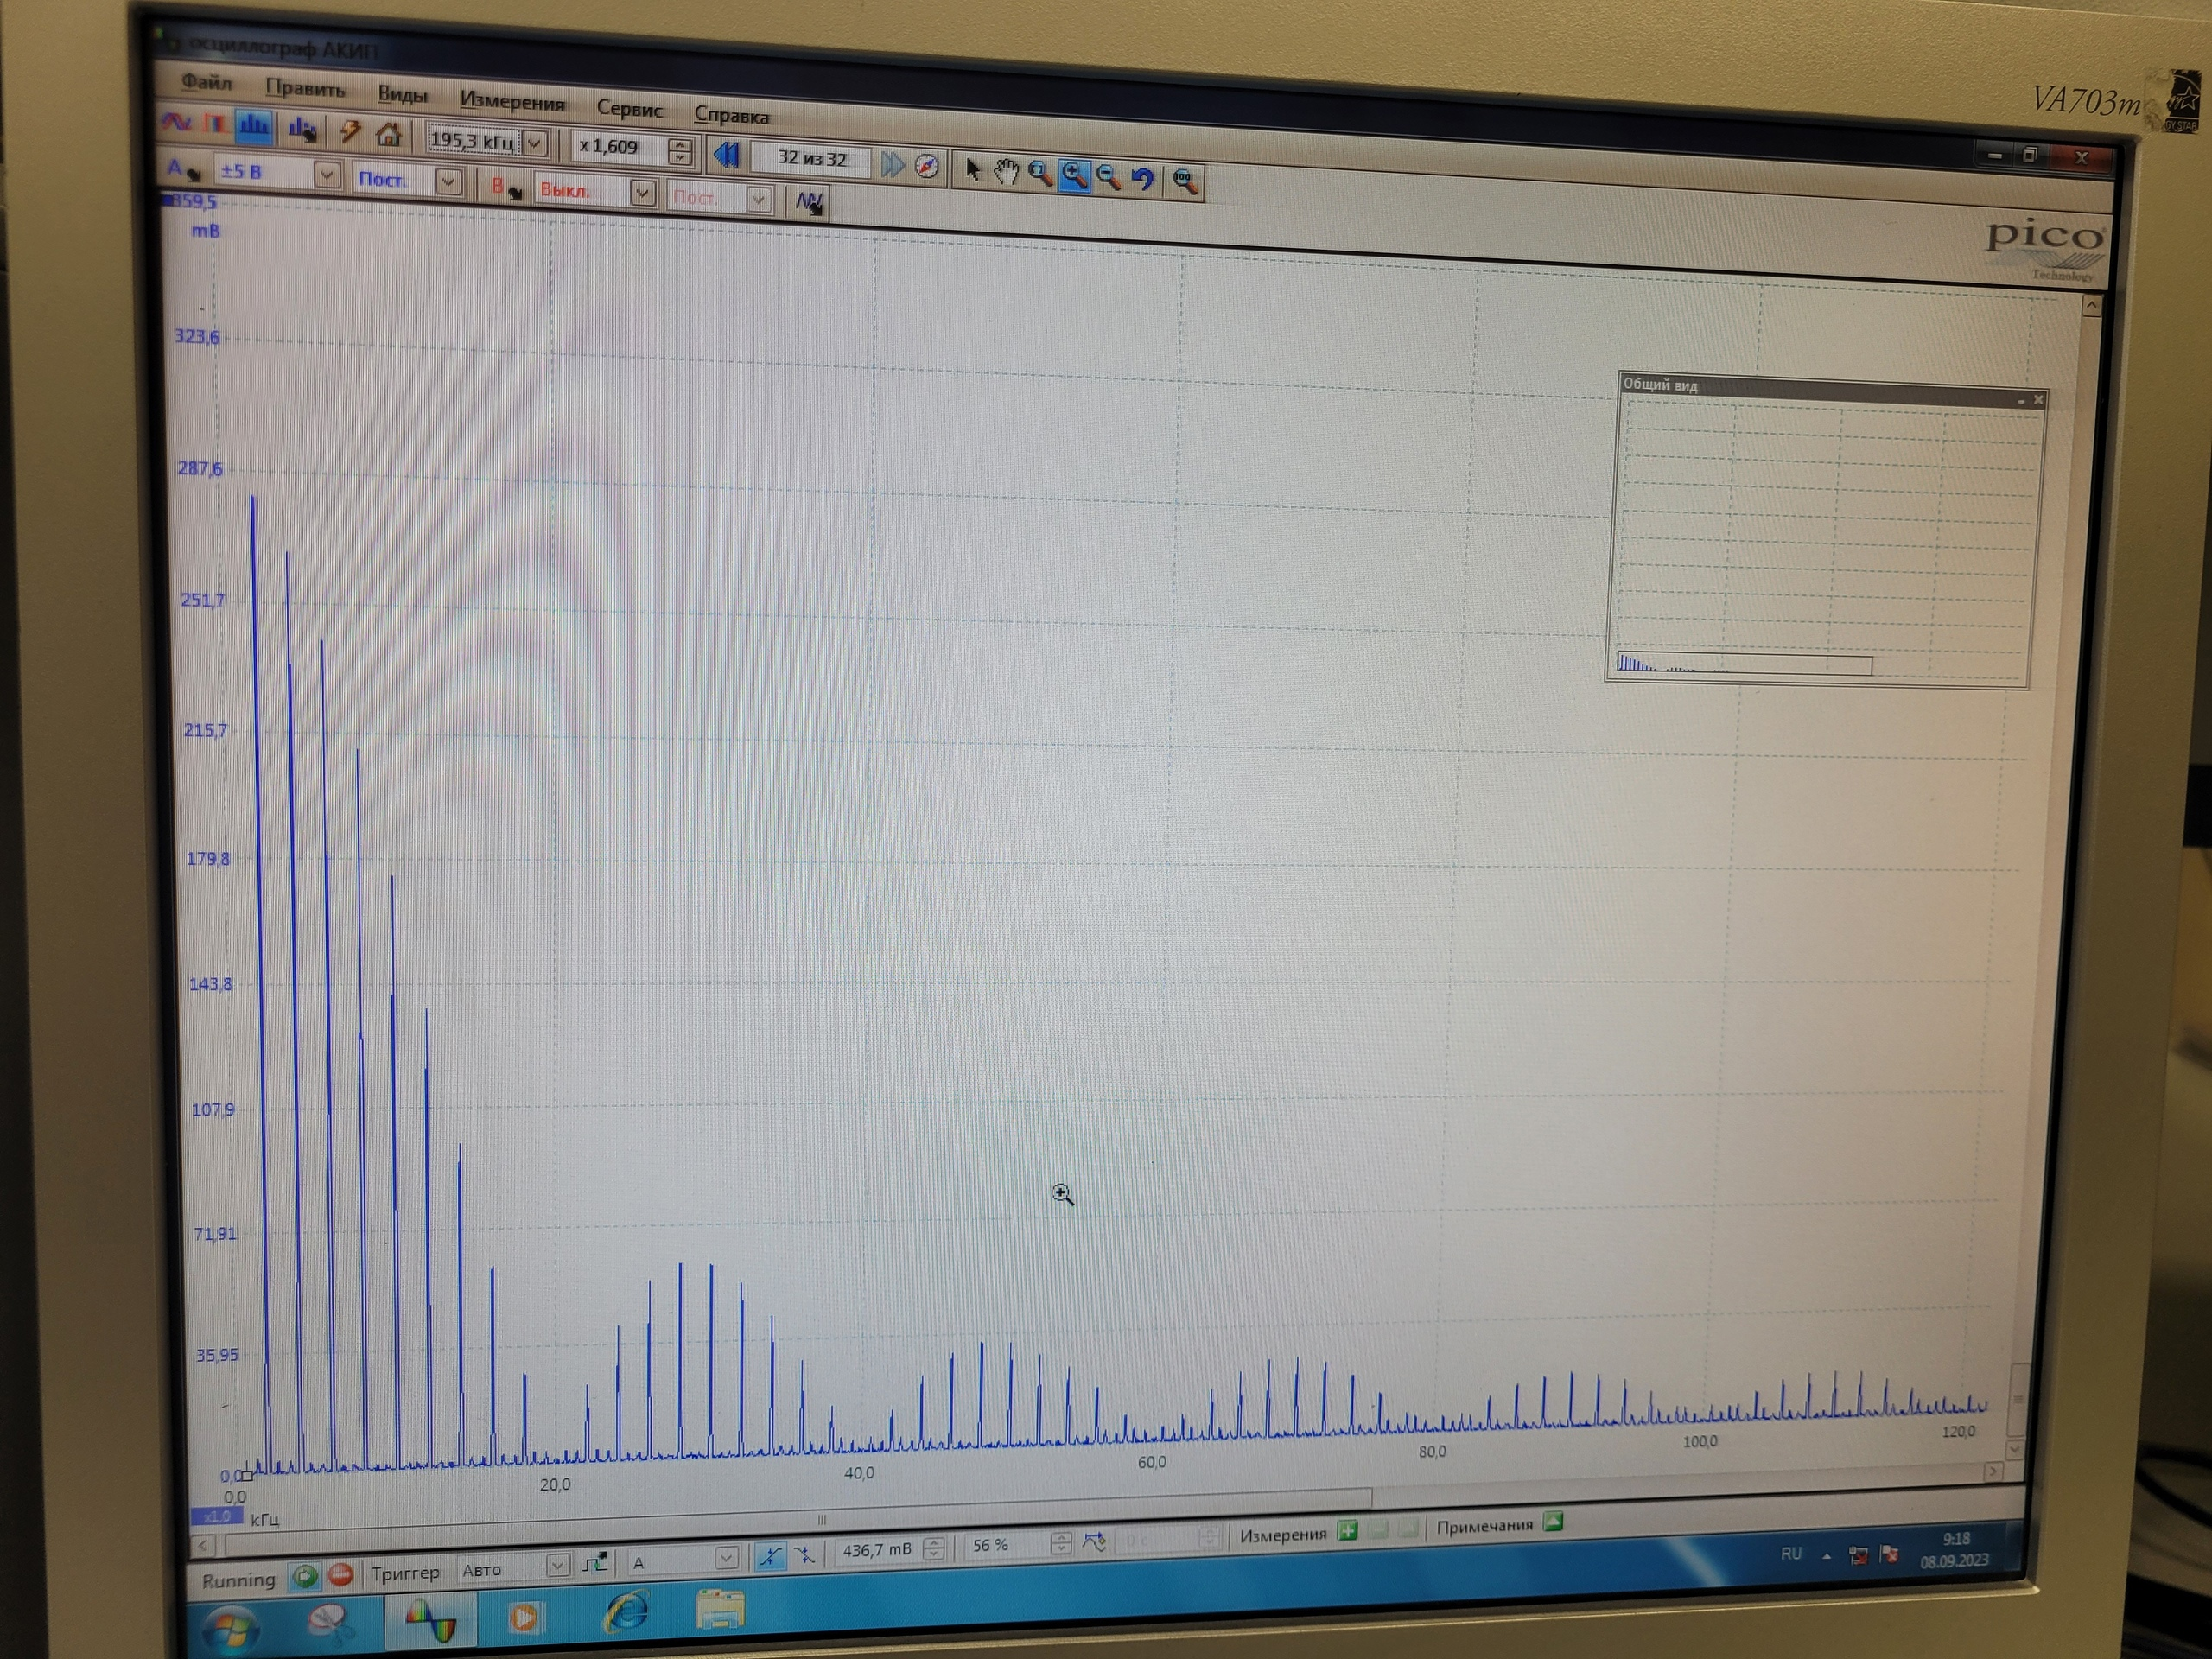
\includegraphics[width=1\linewidth]{A_2k_50.jpg}} \\$\nu_\text{повт}$ = 2 кГц 
\end{minipage}
\vfill
\begin{minipage}[h]{0.47\linewidth}
\center{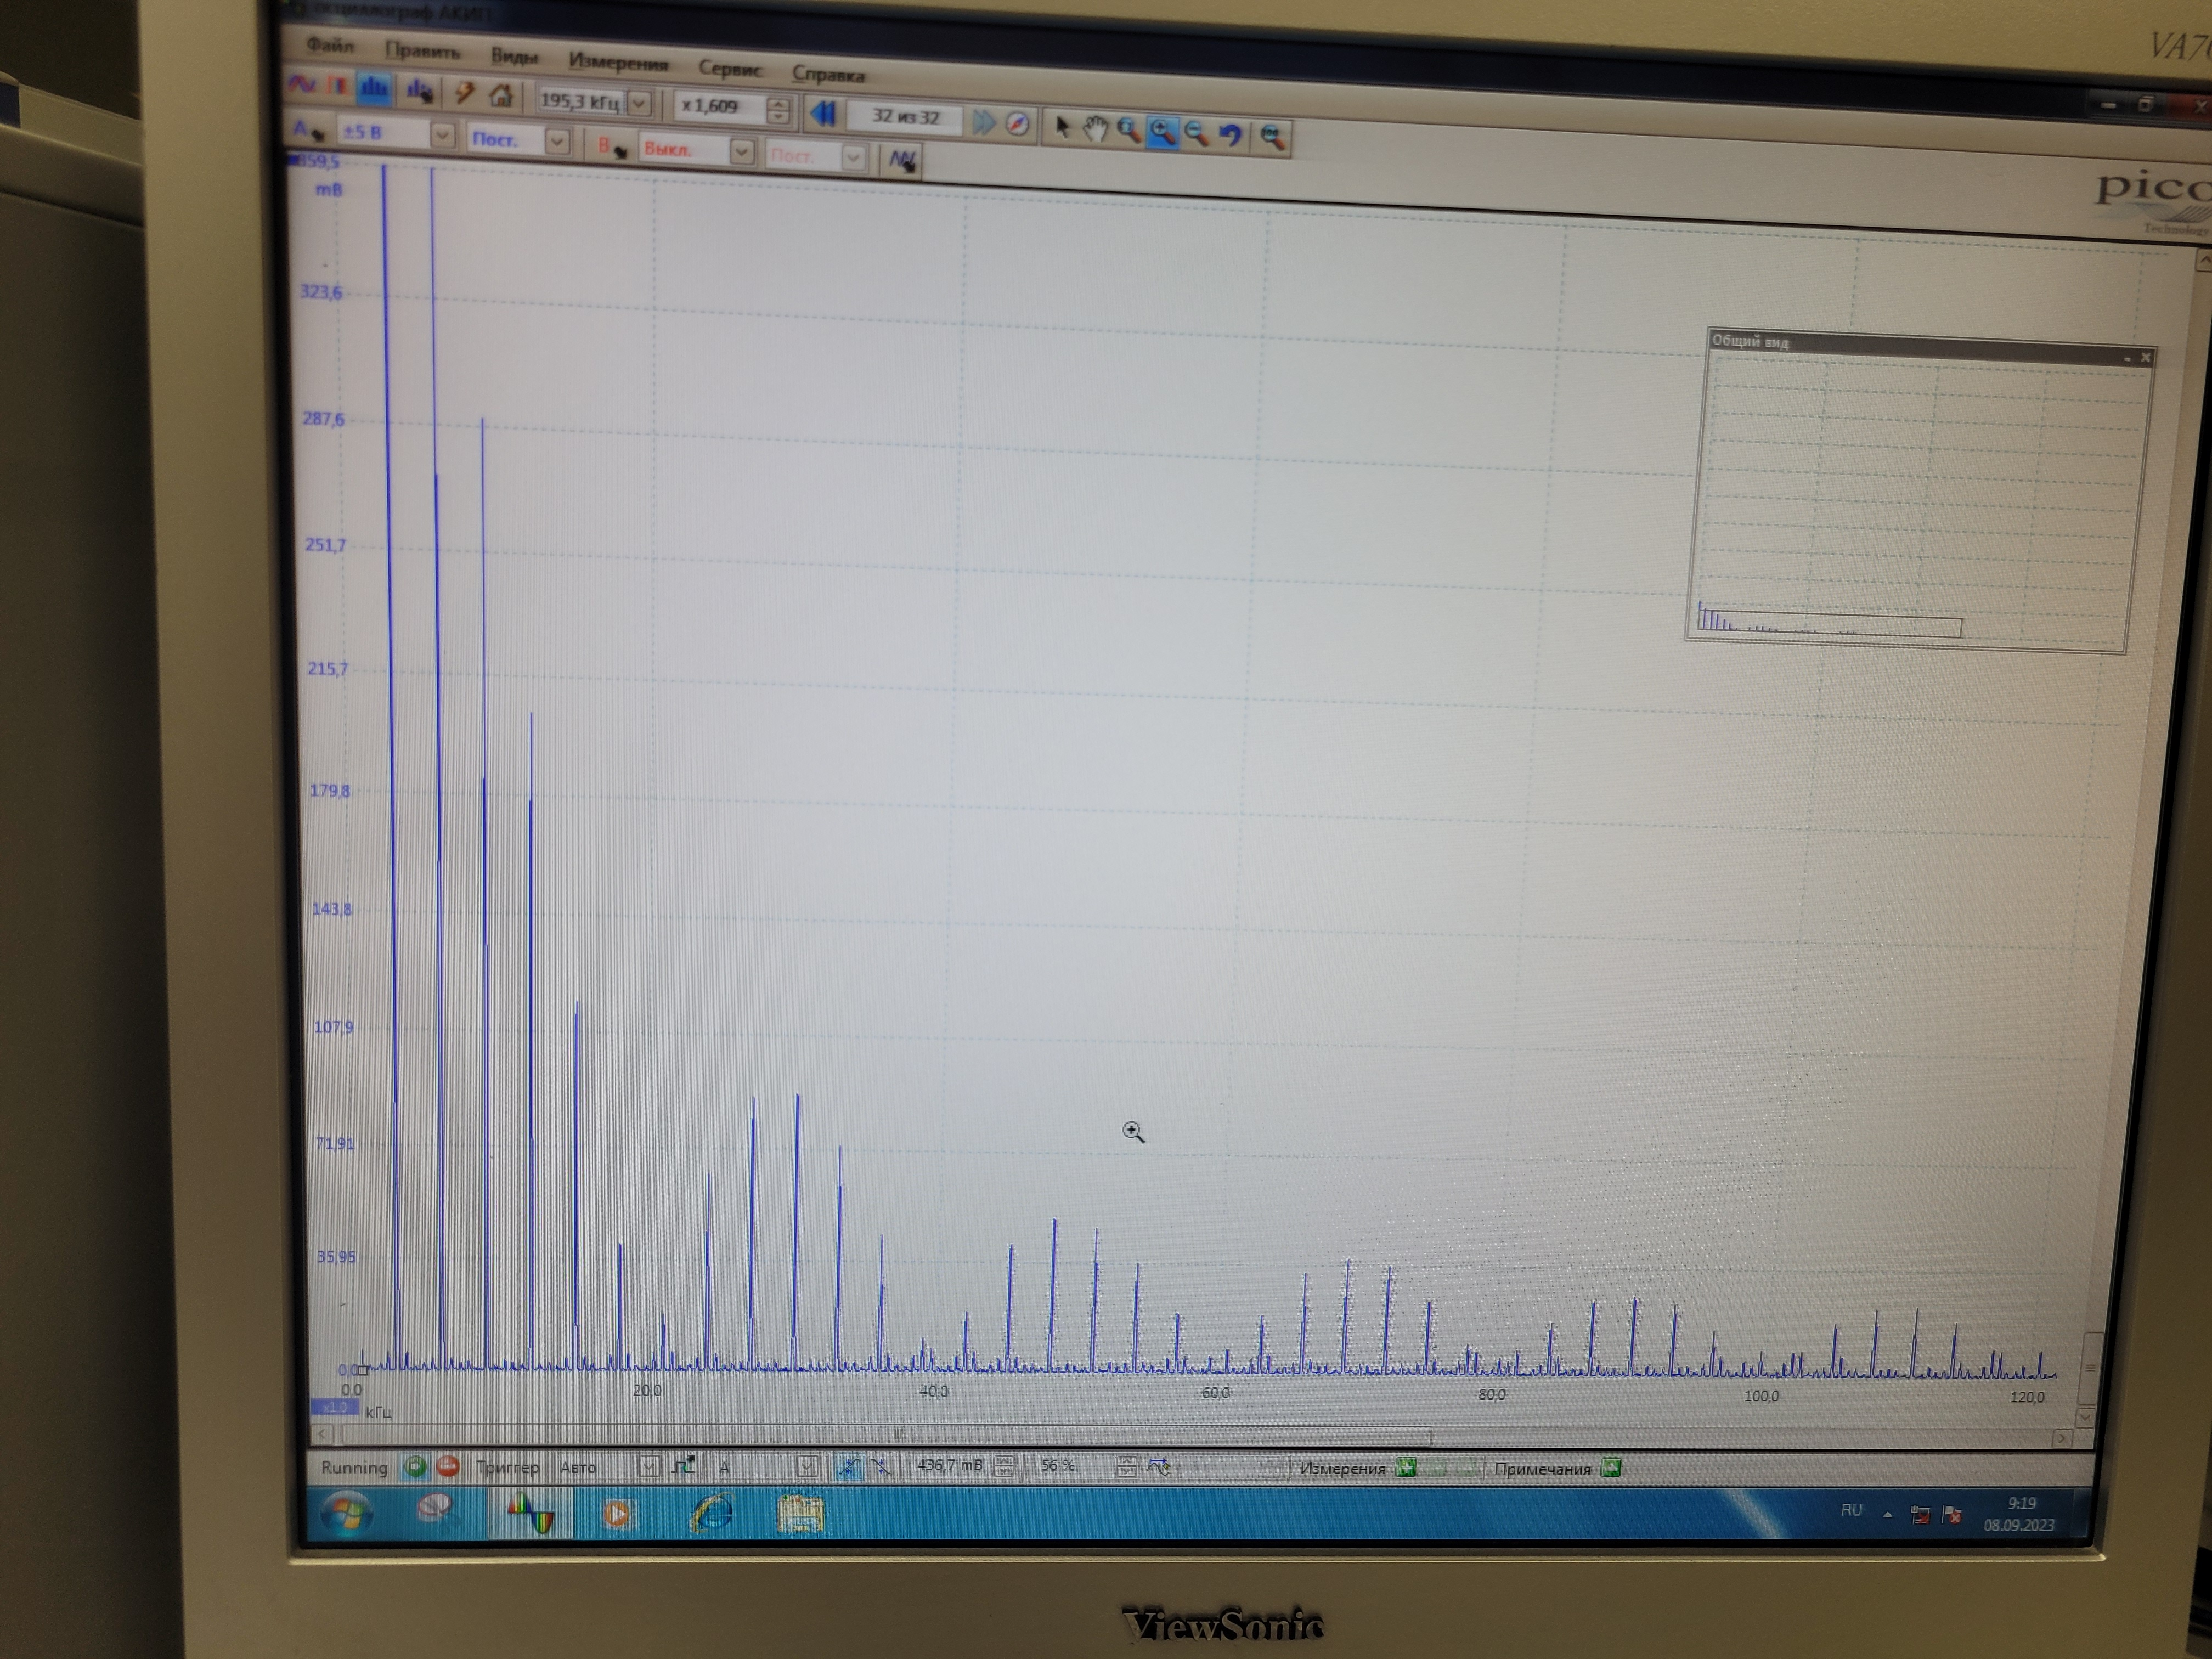
\includegraphics[width=1\linewidth]{A_3k_50.jpg}} $\nu_\text{повт}$ = 3 кГц  \\
\end{minipage}
\hfill
\begin{minipage}[h]{0.47\linewidth}
\center{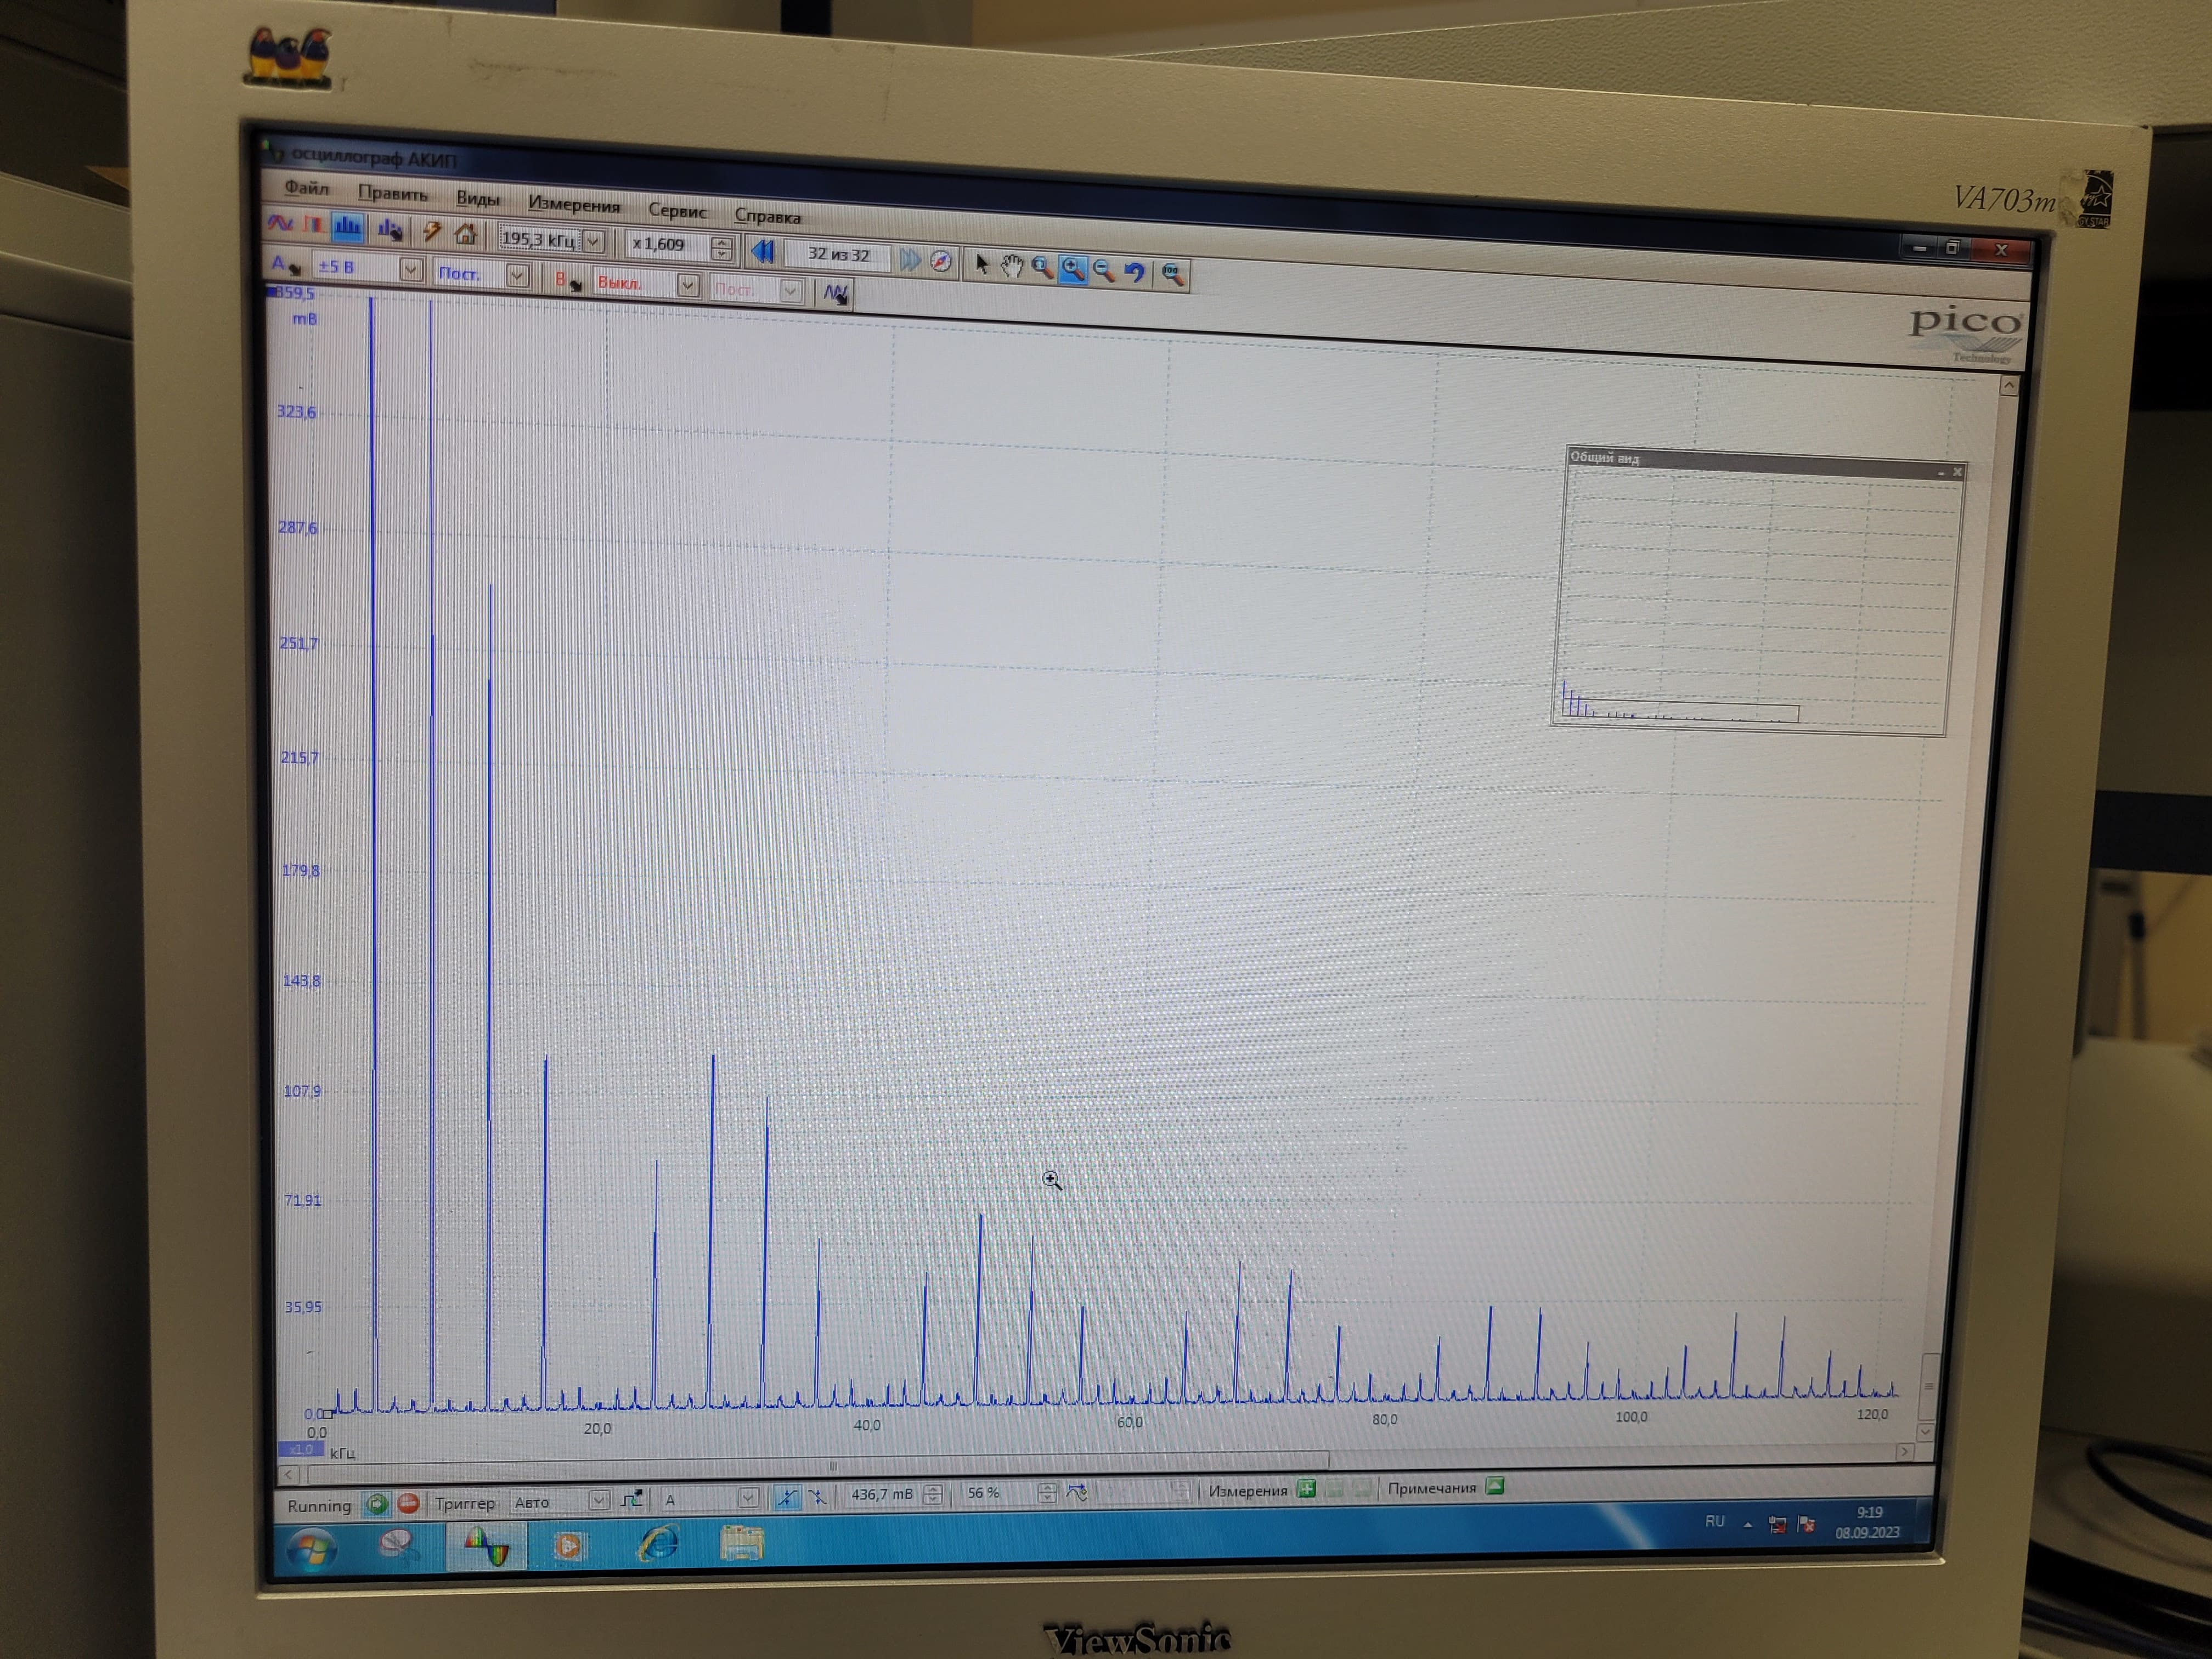
\includegraphics[width=1\linewidth]{A_4k_50.jpg}} $\nu_\text{повт}$ = 4 кГц  \\
\end{minipage}
\caption{}
\label{ris:experimentalcorrelationsignals}
\end{figure}


Как видно из графиков, при увеличении частоты повторения сигнала увеличивается расстояние между компонентами спектра.

\newpage


\textbf{б.} Изменяем $\tau$ при фиксированном $\nu_\text{повт}$ = 1 кГц и получаем:

\begin{figure}[h]
\begin{minipage}[h]{0.47\linewidth}
\center{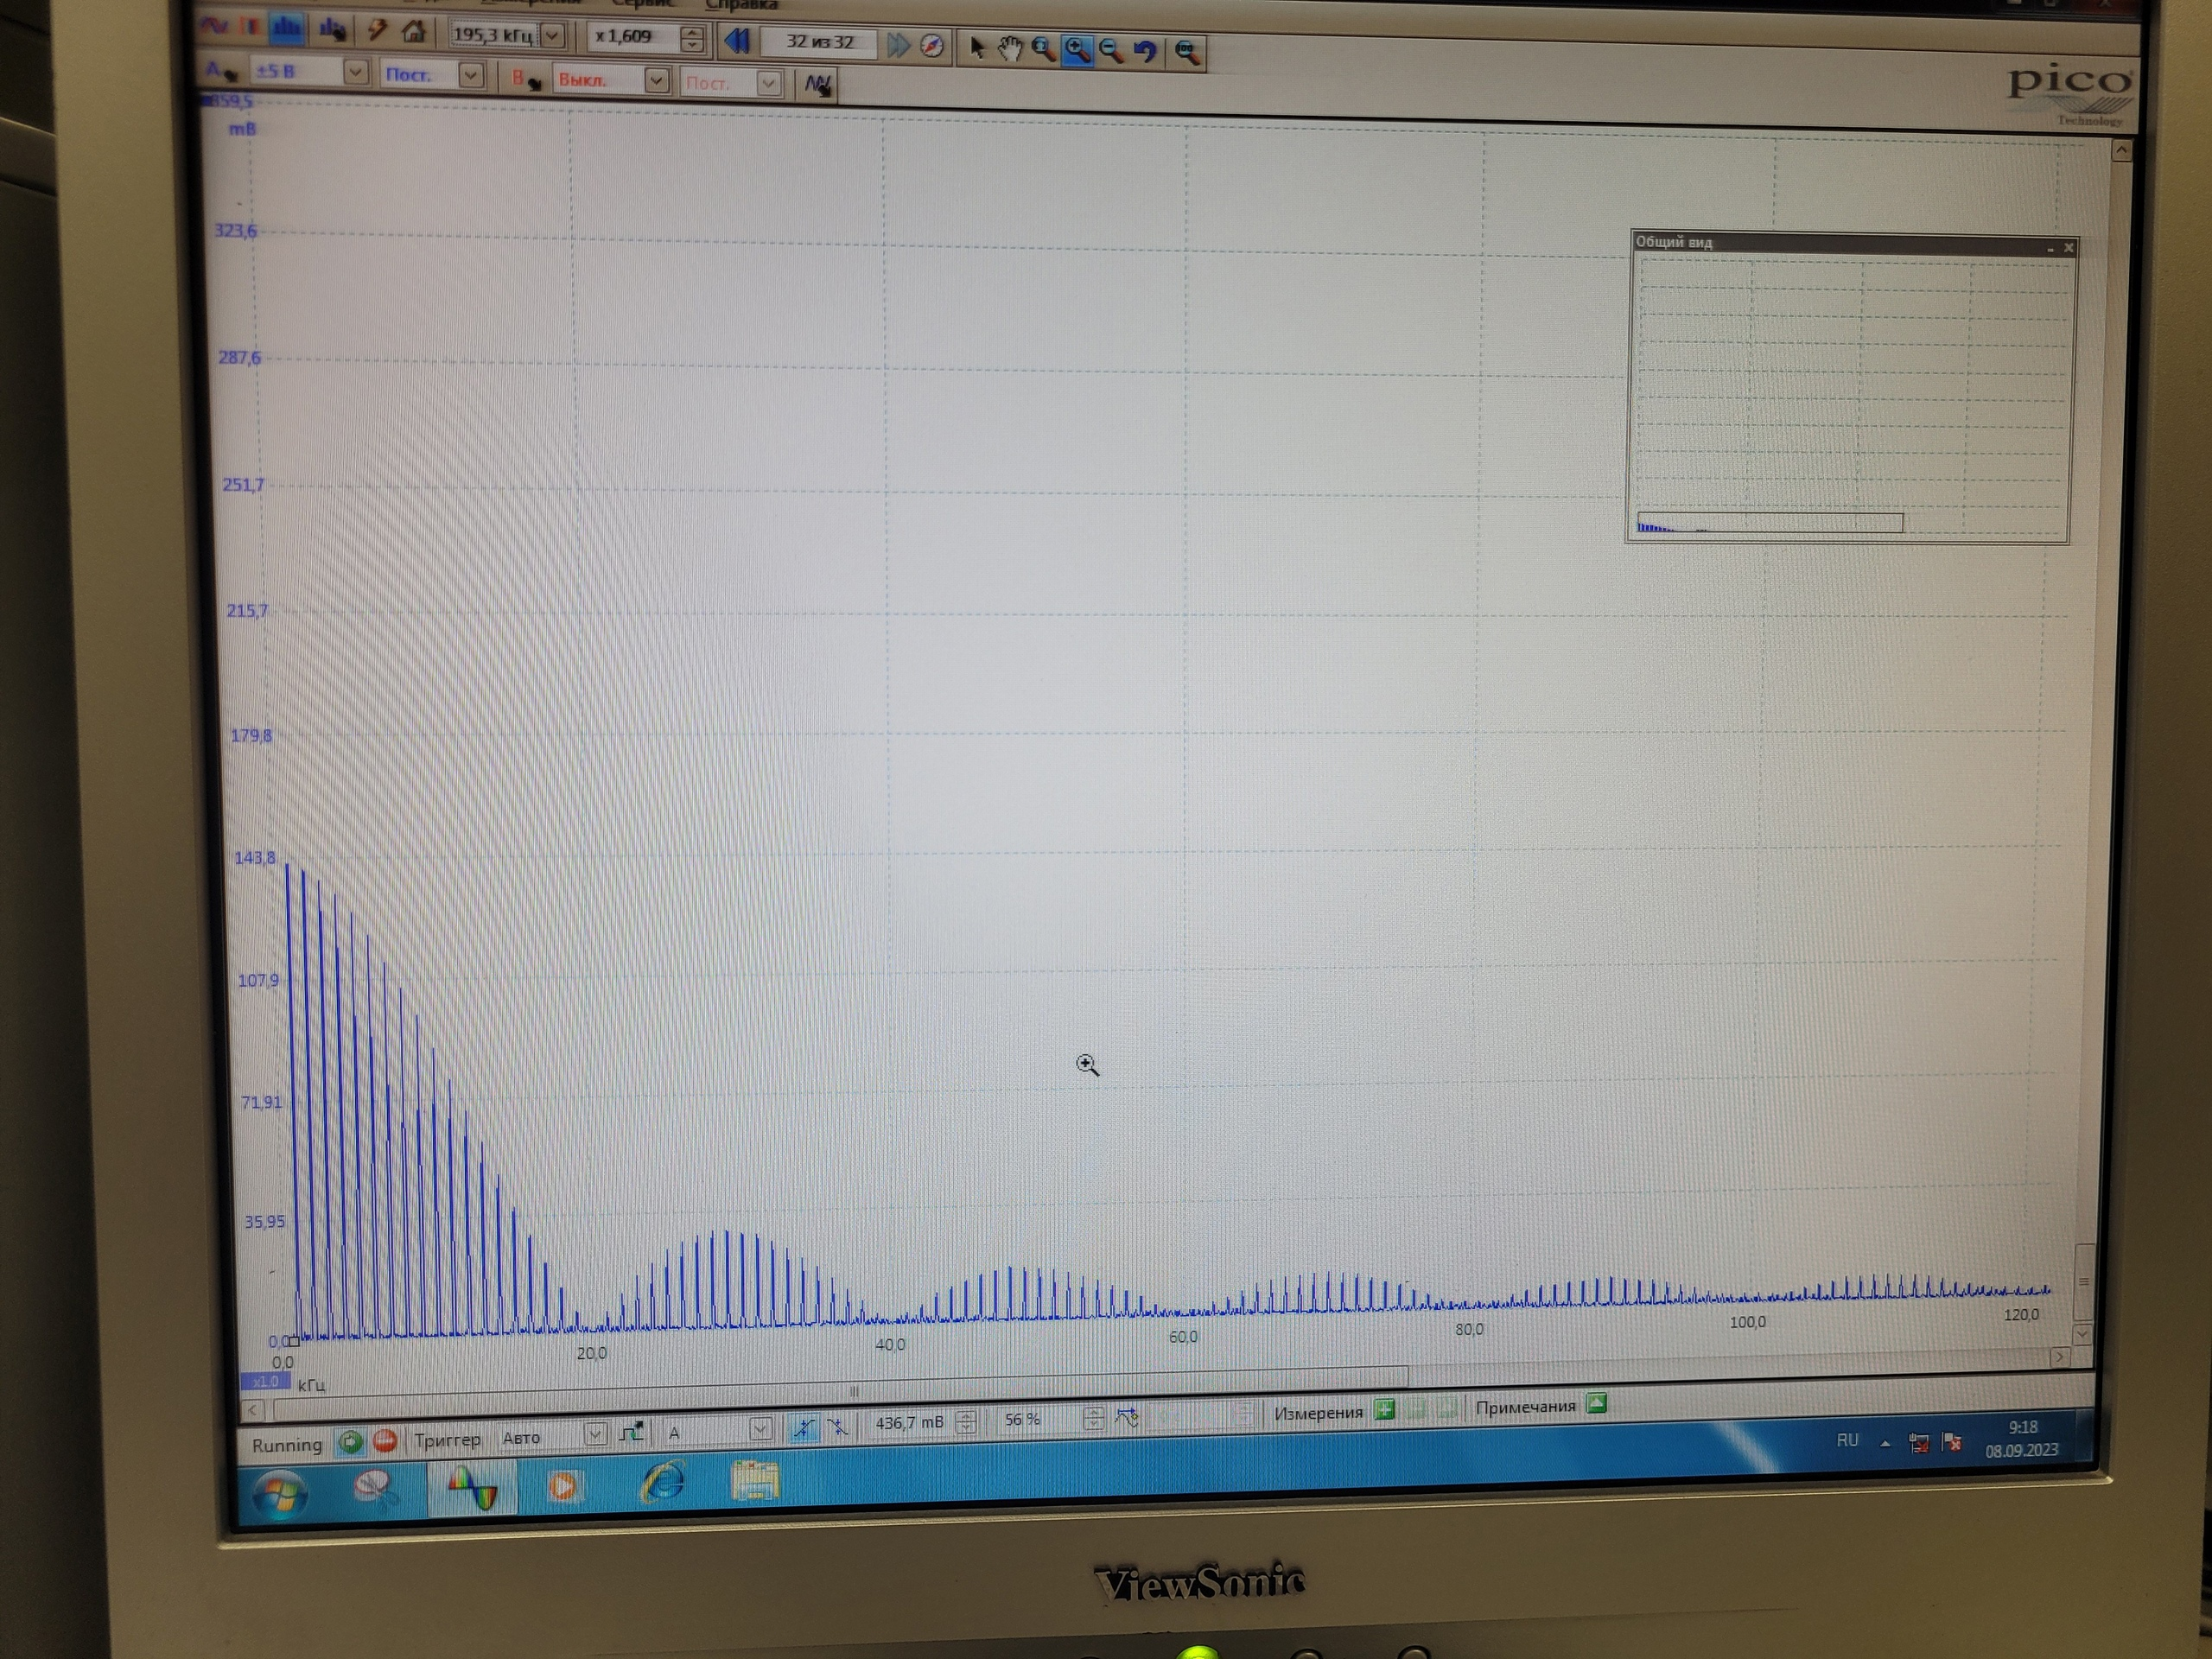
\includegraphics[width=1\linewidth]{A_1k_50.jpg}} $\tau$ = 50 мкс \\
\end{minipage}
\hfill
\begin{minipage}[h]{0.47\linewidth}
\center{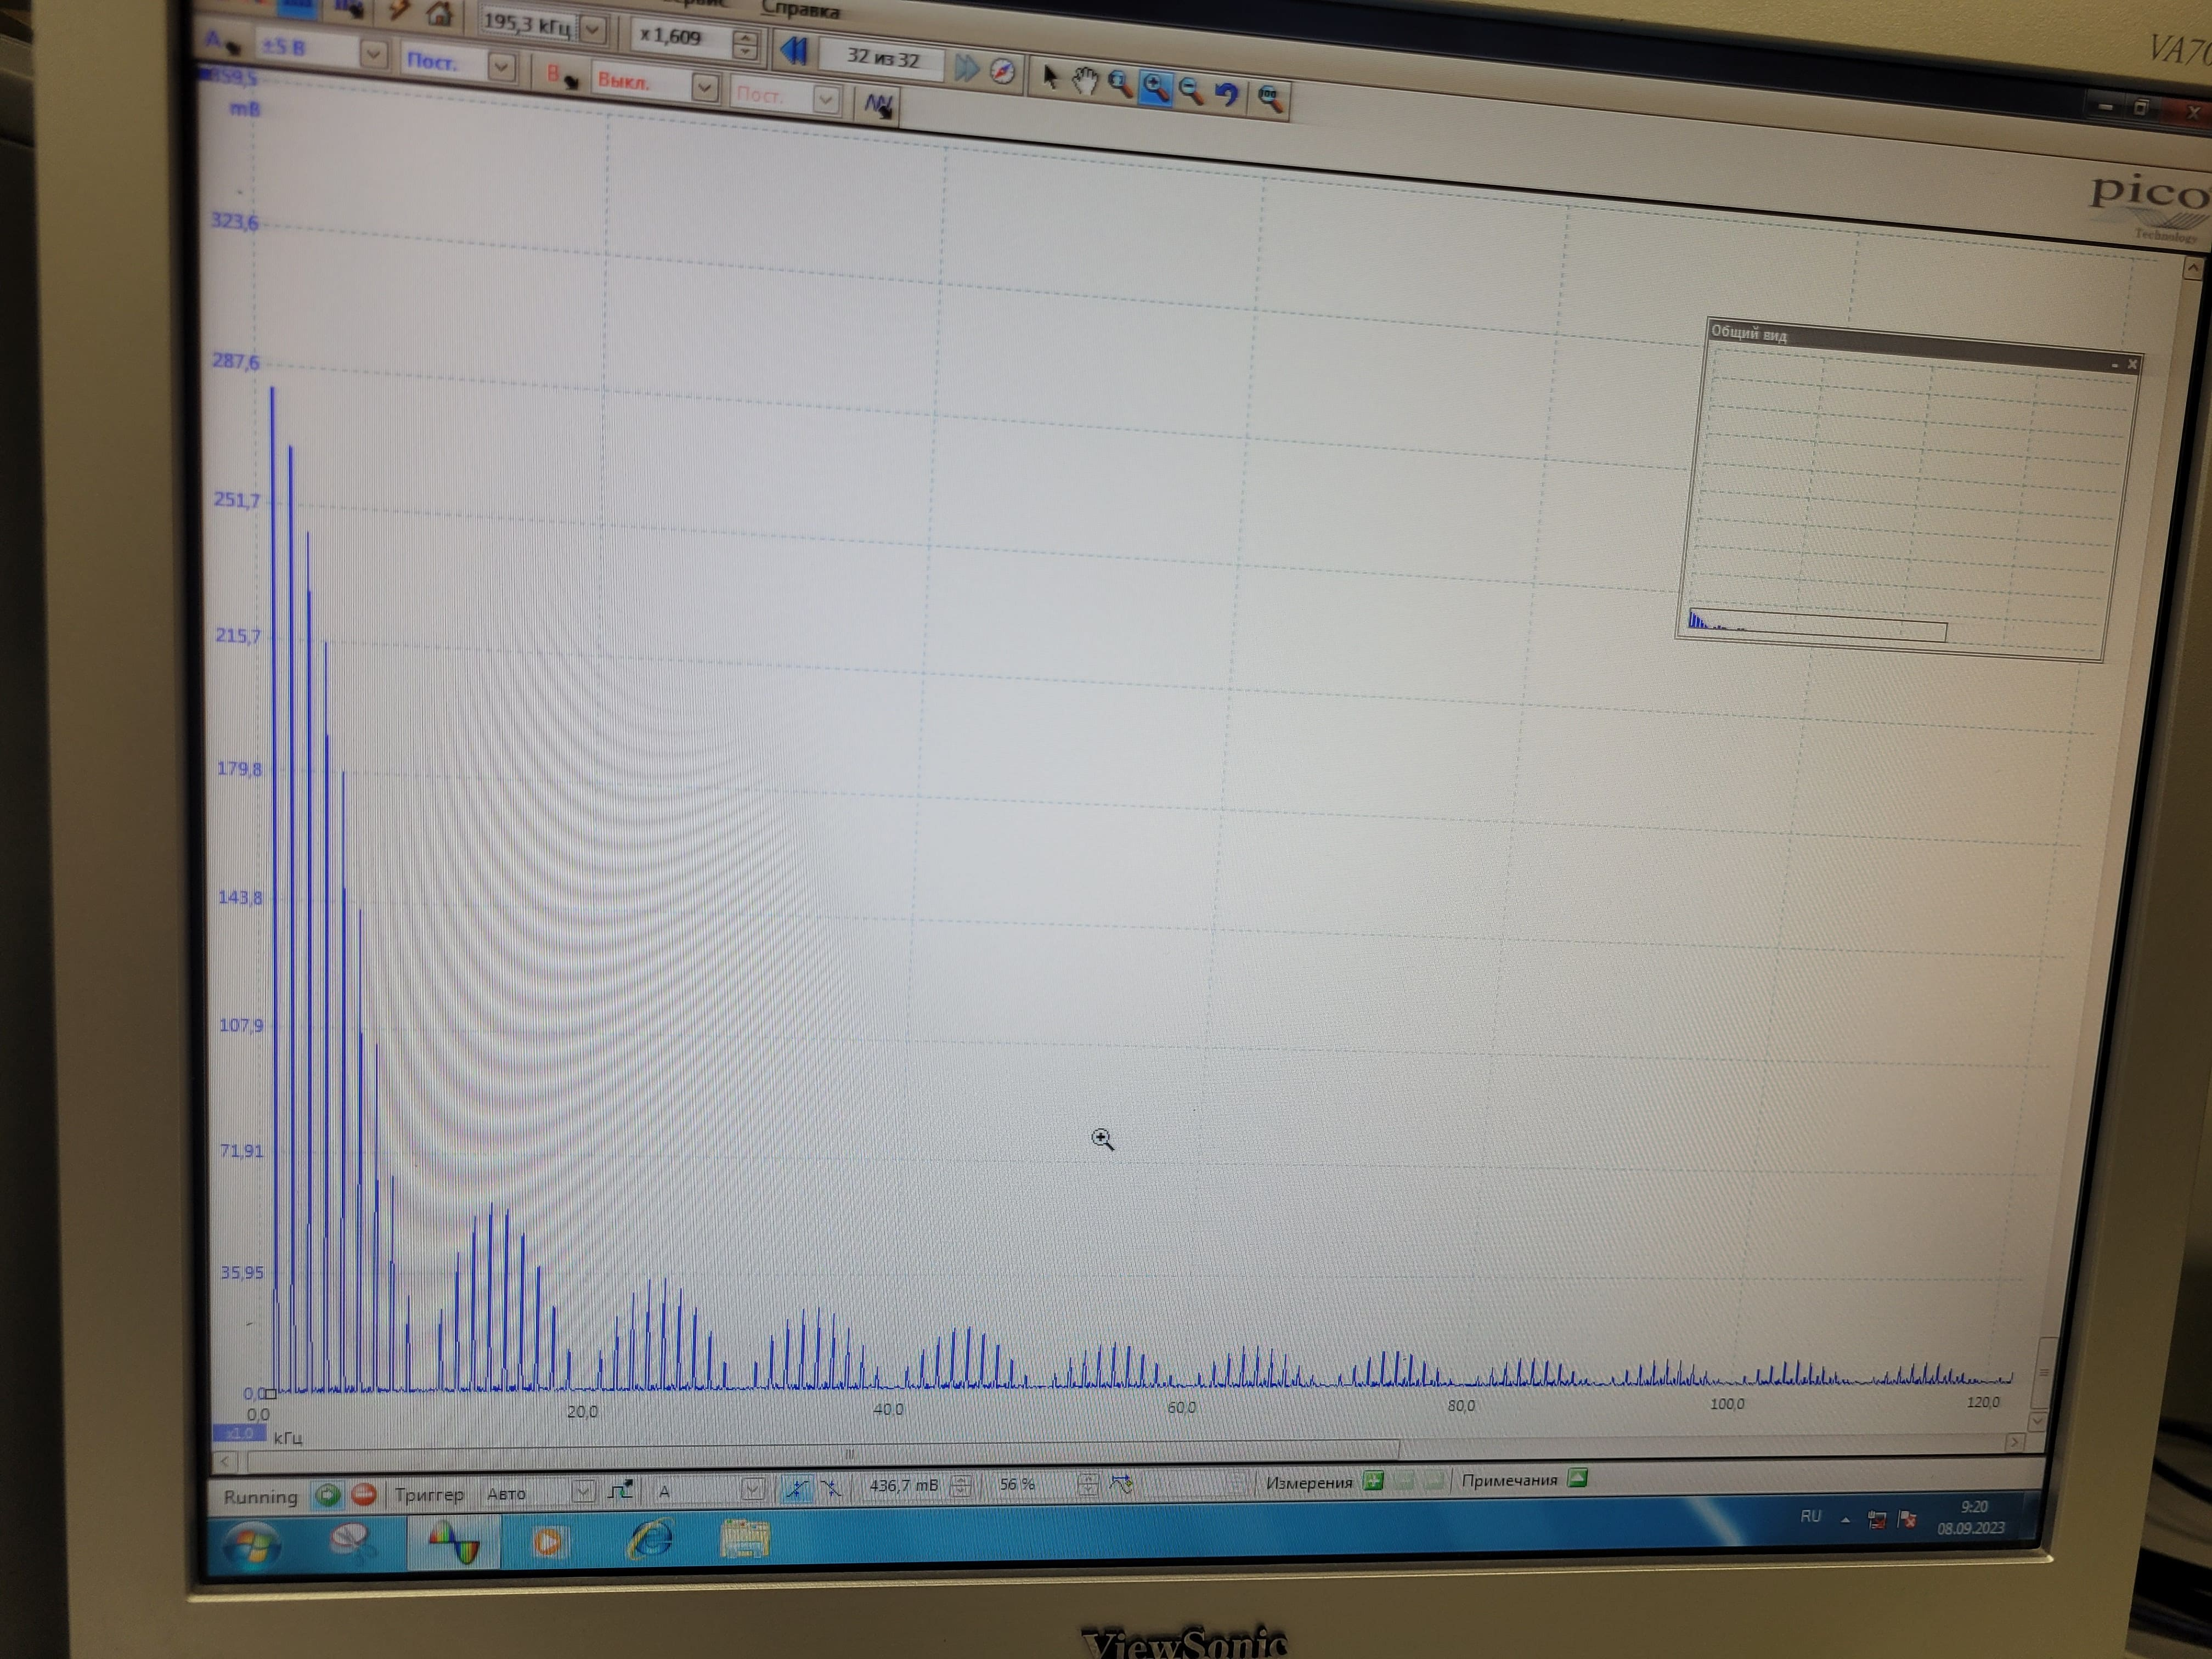
\includegraphics[width=1\linewidth]{A_1k_100.jpg}} \\ $\tau$ = 100 мкс
\end{minipage}
\vfill
\begin{minipage}[h]{0.47\linewidth}
\center{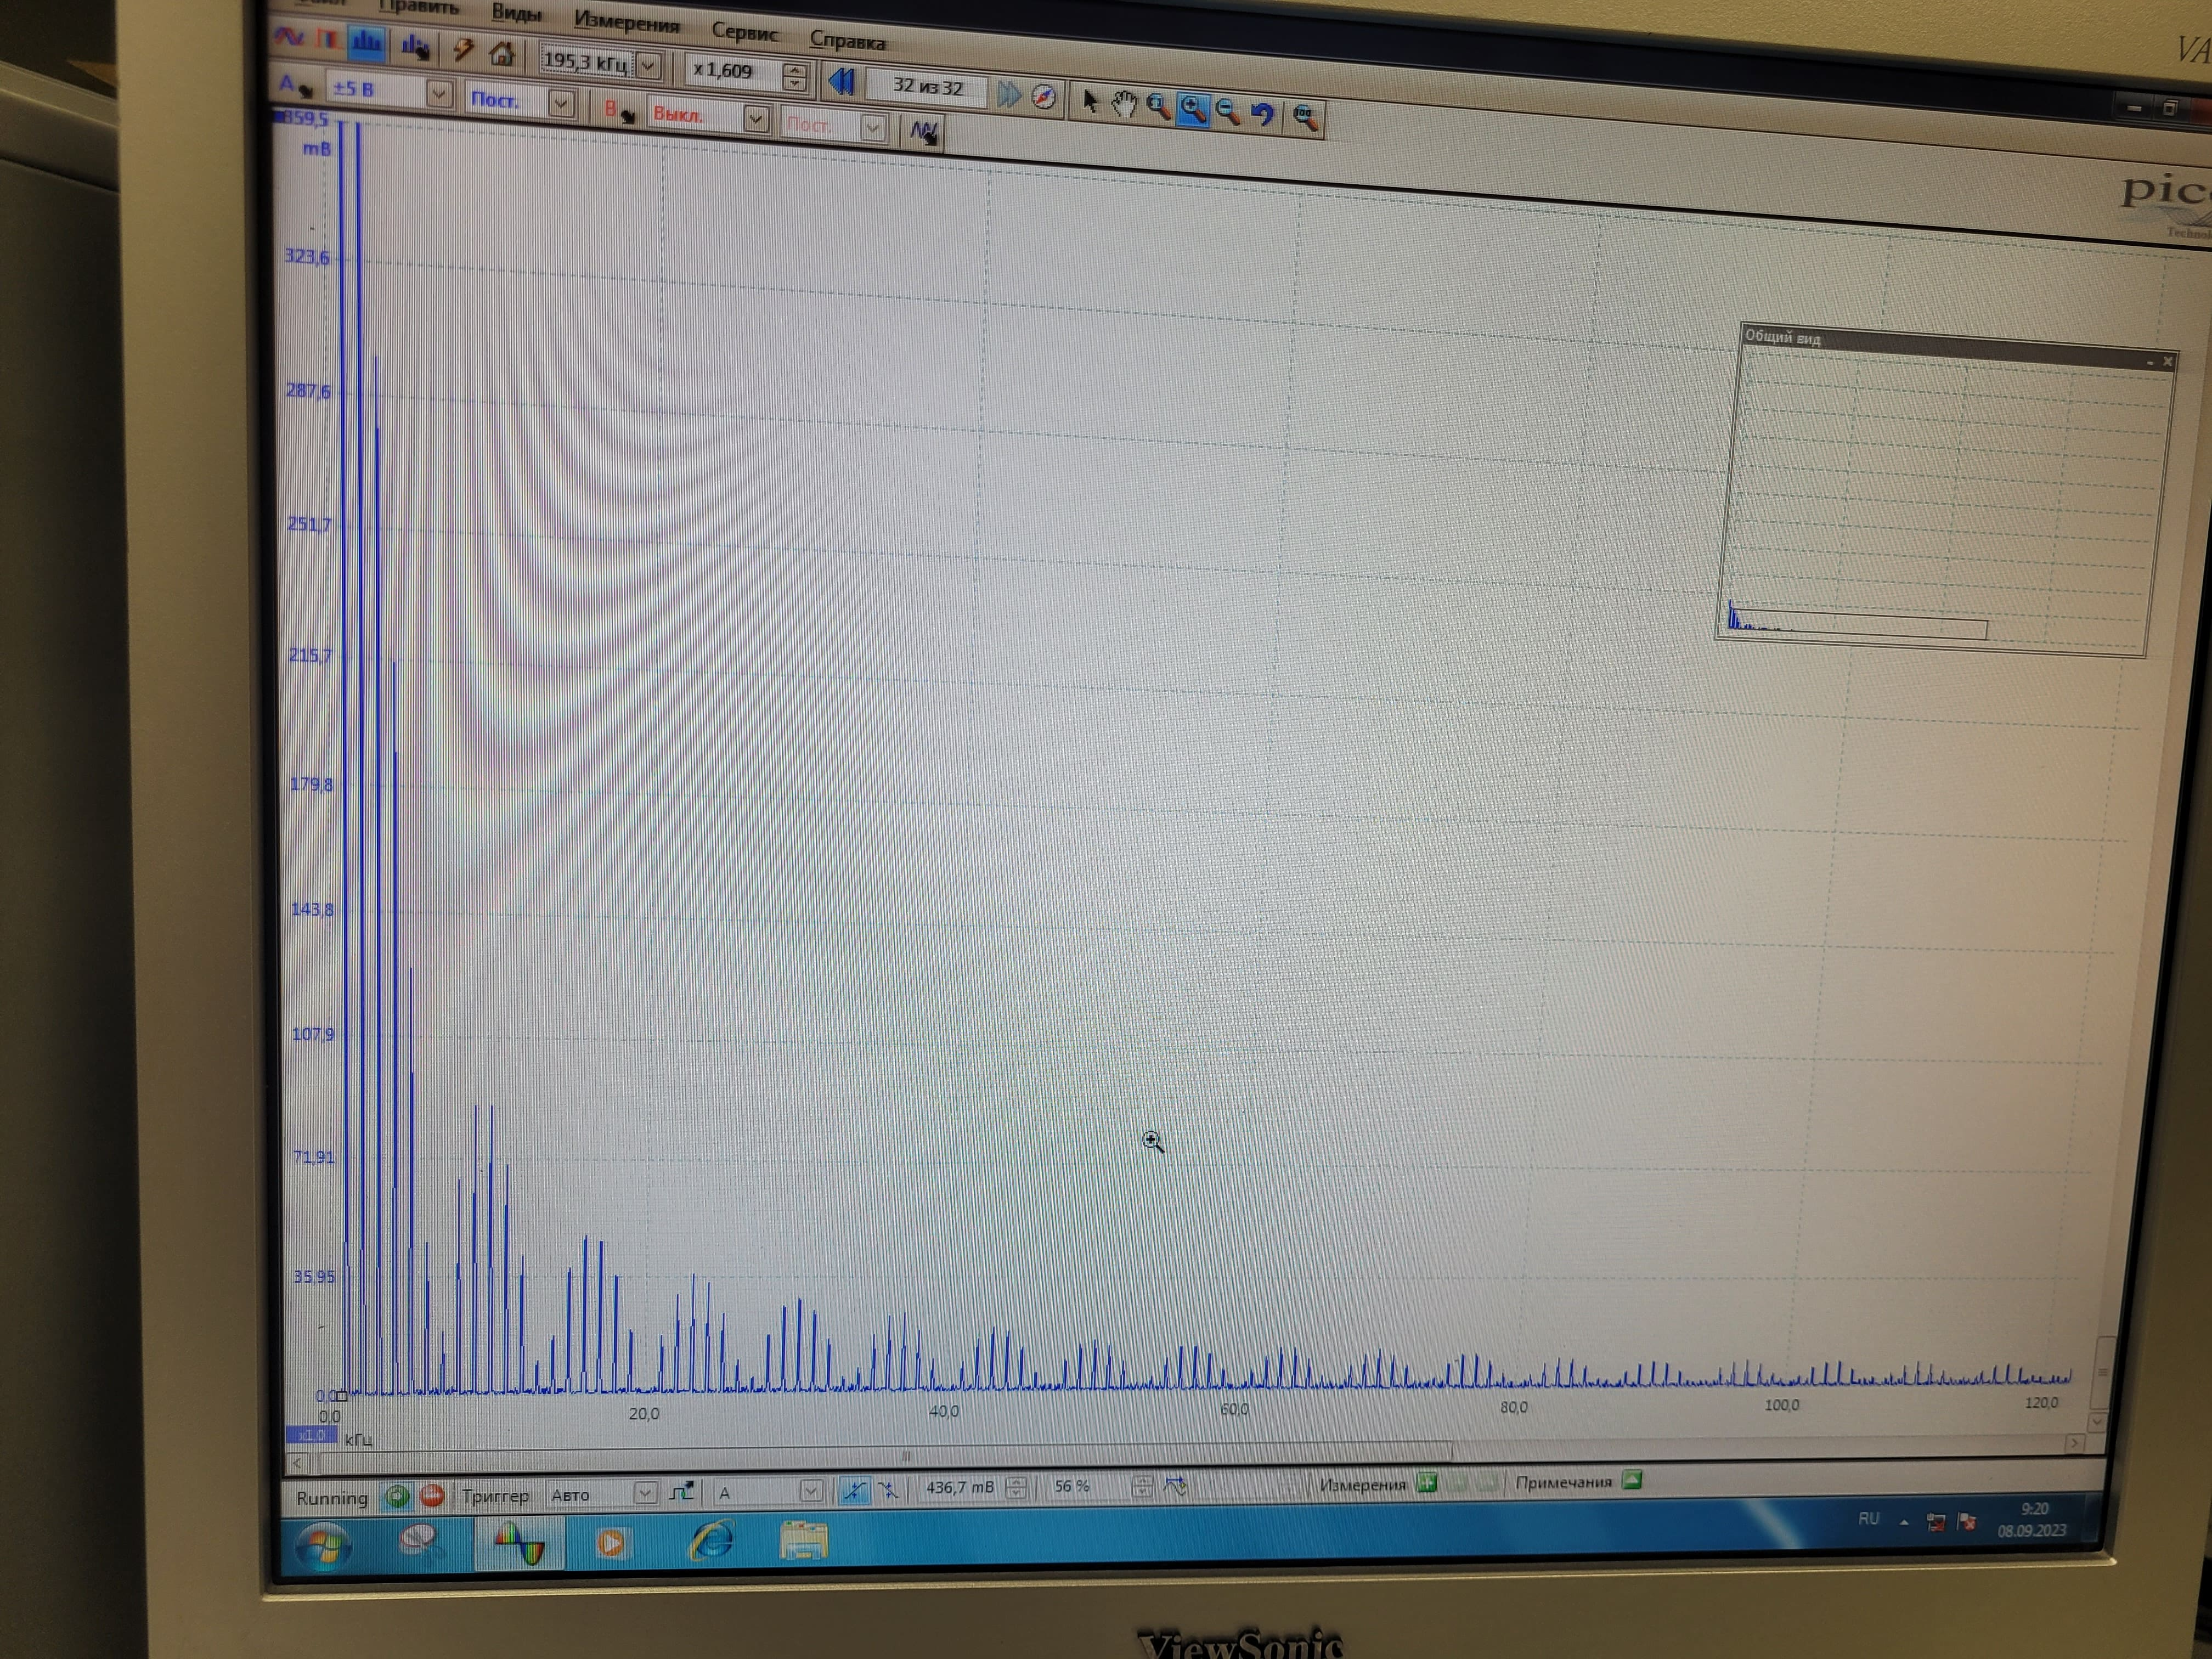
\includegraphics[width=1\linewidth]{A_1k_150.jpg}} $\tau$ = 150 мкс \\ 
\end{minipage}
\caption{}
\label{ris:experimentalcorrelationsignals}
\end{figure}

Как видно из графиков, при увеличении длительности сигнала уменьшается ширина спектра.

\item [\textbf{3.}] Измерим амплитуды $a_n$ и частоты $\nu_n$ спектральных гармоник при фиксированных $\nu_\text{повт}$ и $\tau$.

\begin{table}[!h]
\centering
\begin{tabular}{|l|l|l|l|l|l|l|l|l|}
\hline
$n$ гармоники & 5 & 7 & 9 & 11 & 13 & 15 & 17 & 19 \\ \hline
$\nu_n^\text{эксп}$, кГц & 5.078 & 7.092 & 8.904 & 11.12 & 13.03 & 15.15 & 16.76 & 19.17 \\ \hline
$\nu_n^\text{теор}$, кГц & 5 & 7 & 9 & 11 & 13 & 15 & 17 & 19 \\ \hline
$|a_n|^\text{эксп}$, мВ & 125.9 & 112.3 & 94.73 & 73.98 & 54.58 & 37.44 & 20.75 & 4.962 \\ \hline
$|a_n/a_1|_\text{эксп}$ & 0.876 & 0.781 & 0.659 & 0.515 & 0.380 & 0.261 & 0.144 & 0.034 \\ \hline
$|a_n/a_1|_\text{теор}$ & 0.904 & 0.814 & 0.702 & 0.574 & 0.438 & 0.301 & 0.171 & 0.052 \\ \hline
\end{tabular}
\end{table}

Здесь $a_1$ = 143.8 мВ.
$$\nu_n^\text{теор} = \frac{n}{T}$$
$$|a_n|_\text{теор} = \frac{|\text{sin}\frac{\pi n \tau}{T}|}{\pi n}$$

\item[\textbf{4.}] Зафиксируем период повторения прямоугольного сигнала $T = 1 \text{мс}$, $\nu_\text{повт} = 1\text{кГц}$. Изменяя длительность импульса $\tau$ в диапазоне от 
$\tau=T/50$ до $\tau=T/5$, измерим полную ширину спектра сигнала $\Delta \nu$ — от центра спектра ($\nu = 0$) до гармоники с нулевой амплитудой $a_n \approx 0$ и установим зависимость между $\Delta \nu$ и $\tau$, полученную из формулы \ref{eq5}.

\begin{table}[h!]
    \centering
    \begin{tabular}{|c|c|c|c|c|c|c|c|}
\hline
$\tau$, мкс & 20 & 25 & 40 & 50 & 100 & 150 & 200 \\ \hline
$\Delta \nu$, кГц & 49.68 & 39.71 & 24.61 & 19.98 & 9.91 & 6.84 & 4.93 \\ \hline
$1/\tau \cdot 10^3$, с$^{-1}$ & 50 & 40 & 25 & 20 & 10 & 7 & 5 \\ \hline
\end{tabular}
    \caption{Исследование зависимости $\Delta \nu$ и $\tau$}
    \label{table2}
\end{table}
Построим график $\Delta\nu\left(\frac{1}{\tau}\right)$. Используя МНК, получим $k=0.994\pm0,002$, откуда с хорошей точностью можем заключить, что $\Delta\nu\frac{1}{\tau}=1$, что экспериментально доказывает соотношение неопределённостей. График приведён на рис.12
\begin{figure}[h]
    \centering
    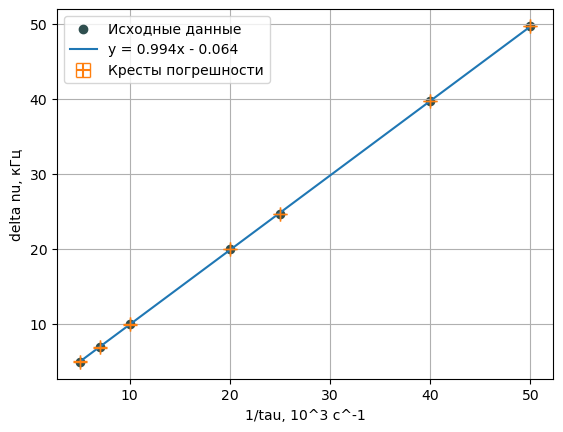
\includegraphics[width=0.7\linewidth]{grafic1.png}
    \caption{Зависимость $\Delta \nu$ от $1/\tau$}
    \label{grafic1}
\end{figure}

\item[\textbf{5.}] 
Зафиксируем длительность импульса прямоугольного сигнала $\tau = 100 \text{мкс}$. Изменяя период повторения $T$ в диапазоне от $2\tau$ до $50\tau$ измерим расстояния $\delta\nu = \nu_{n+1} - \nu_n$ между соседними гармониками спектра. 
\begin{table}[h!]
    \centering
    \begin{tabular}{|c|c|c|c|c|c|c|}
\hline
$\nu$, кГц & 5 & 2 & 1 & 0.5 & 0.25 & 0.1 \\ \hline
$\delta \nu$, кГц & 5.036 & 1.927 & 1.008 & 0.510 & 0.253 & 0.206 \\ \hline
\end{tabular}
    \caption{Зависимость $\delta \nu$ от $1/T$}
    \label{table3}
\end{table}

\newpage

\begin{figure}[h]
    \centering
    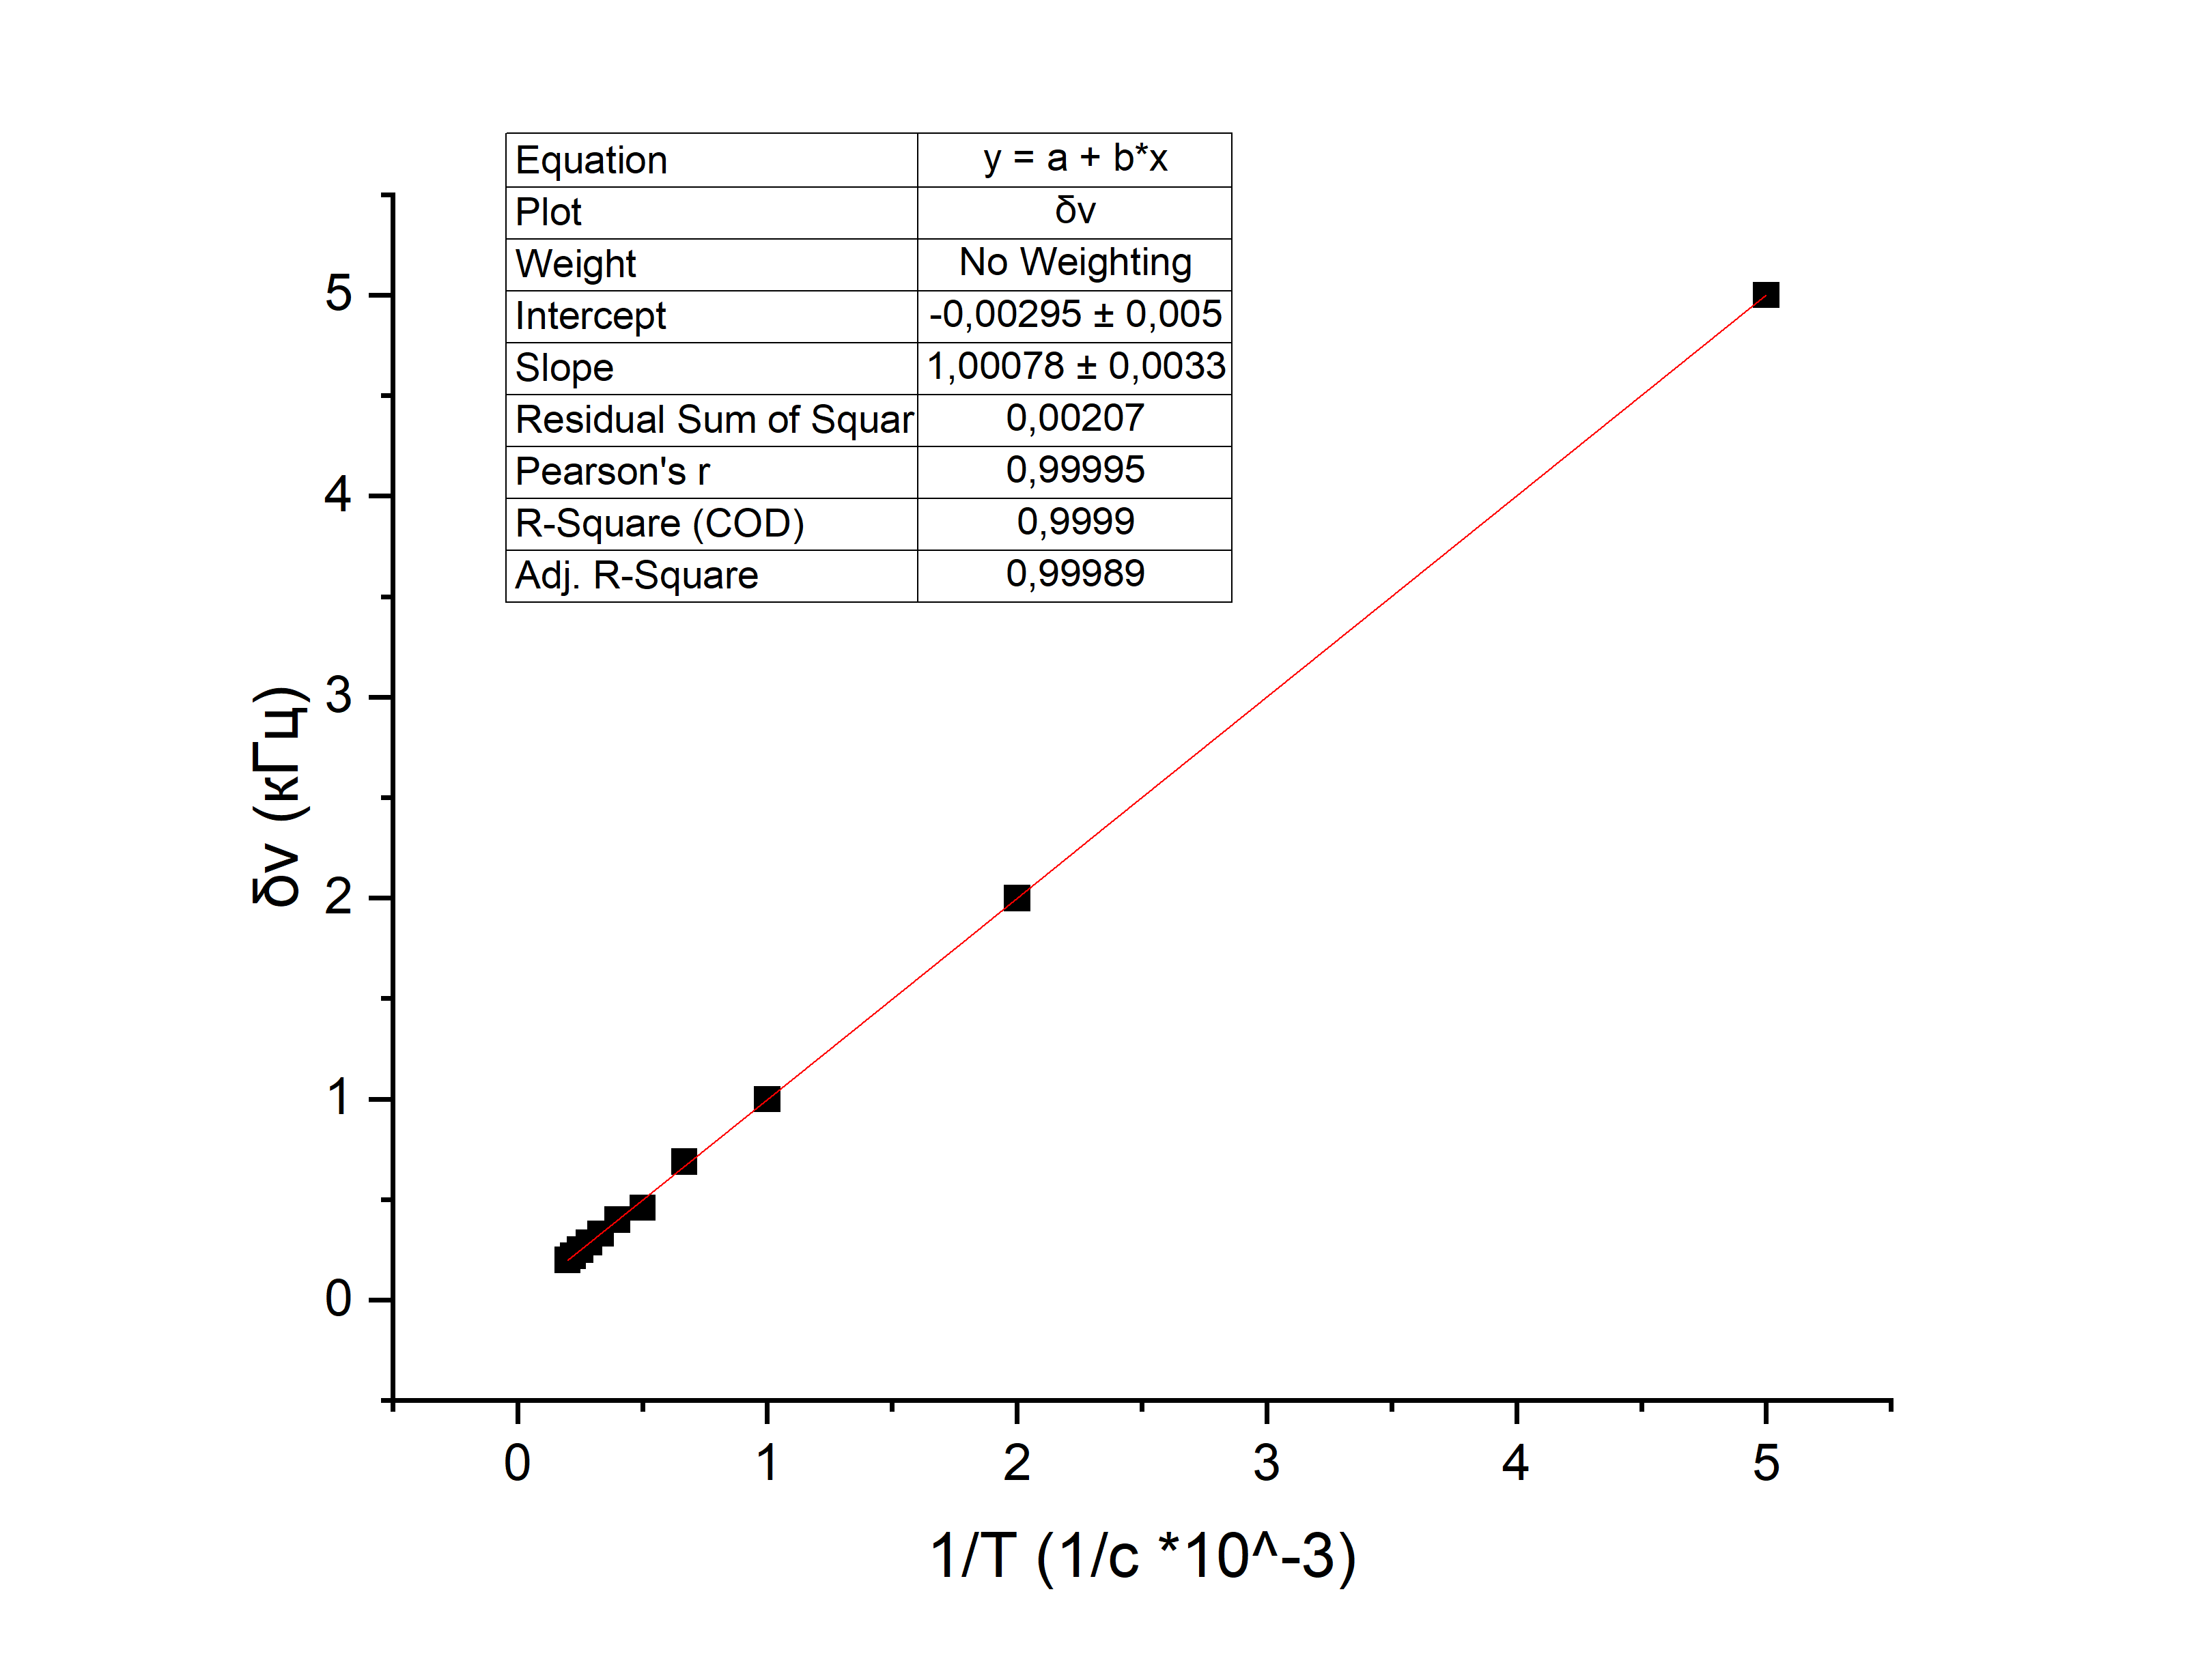
\includegraphics[width=0.7\linewidth]{grafic2.png}
    \caption{Зависимость $\delta \nu$ от $1/T$}
    \label{grafic2}
\end{figure}
Построим график $\delta\nu\left(\frac{1}{T}\right)$. Используя МНК, получим $k=0.996\pm0,013$, что экспериментально доказывает соотношение неопределённостей. График приведён на рис.13.
\end{enumerate}


\newpage

\subsection*{Б. Наблюдение спектра периодической последовательности цугов}

\begin{enumerate}
\item [\textbf{1.}] Настраиваем генератор на периодичные импульсы синусоидальной формы (цугов) с несущей частотой $\nu_0$ = 50 кГц, частотой повторения $\nu_\text{повт}$ = 1 кГц, число периодов синусоиды в одном импульсе $N$ = 5 (что соответствует длительности импульса $\tau$ = $N/\nu_o$ = 100 мкс).

\item [\textbf{2.}] Получаем на экране спектр (Преобразование Фурье) сигнала.

\textbf{a.} Изменяем $N$ при фиксированных $\nu_0$ = 50 кГц и $\nu_\text{повт}$ = 1 кГц:

\begin{figure}[h]
\begin{minipage}[h]{0.47\linewidth}
\center{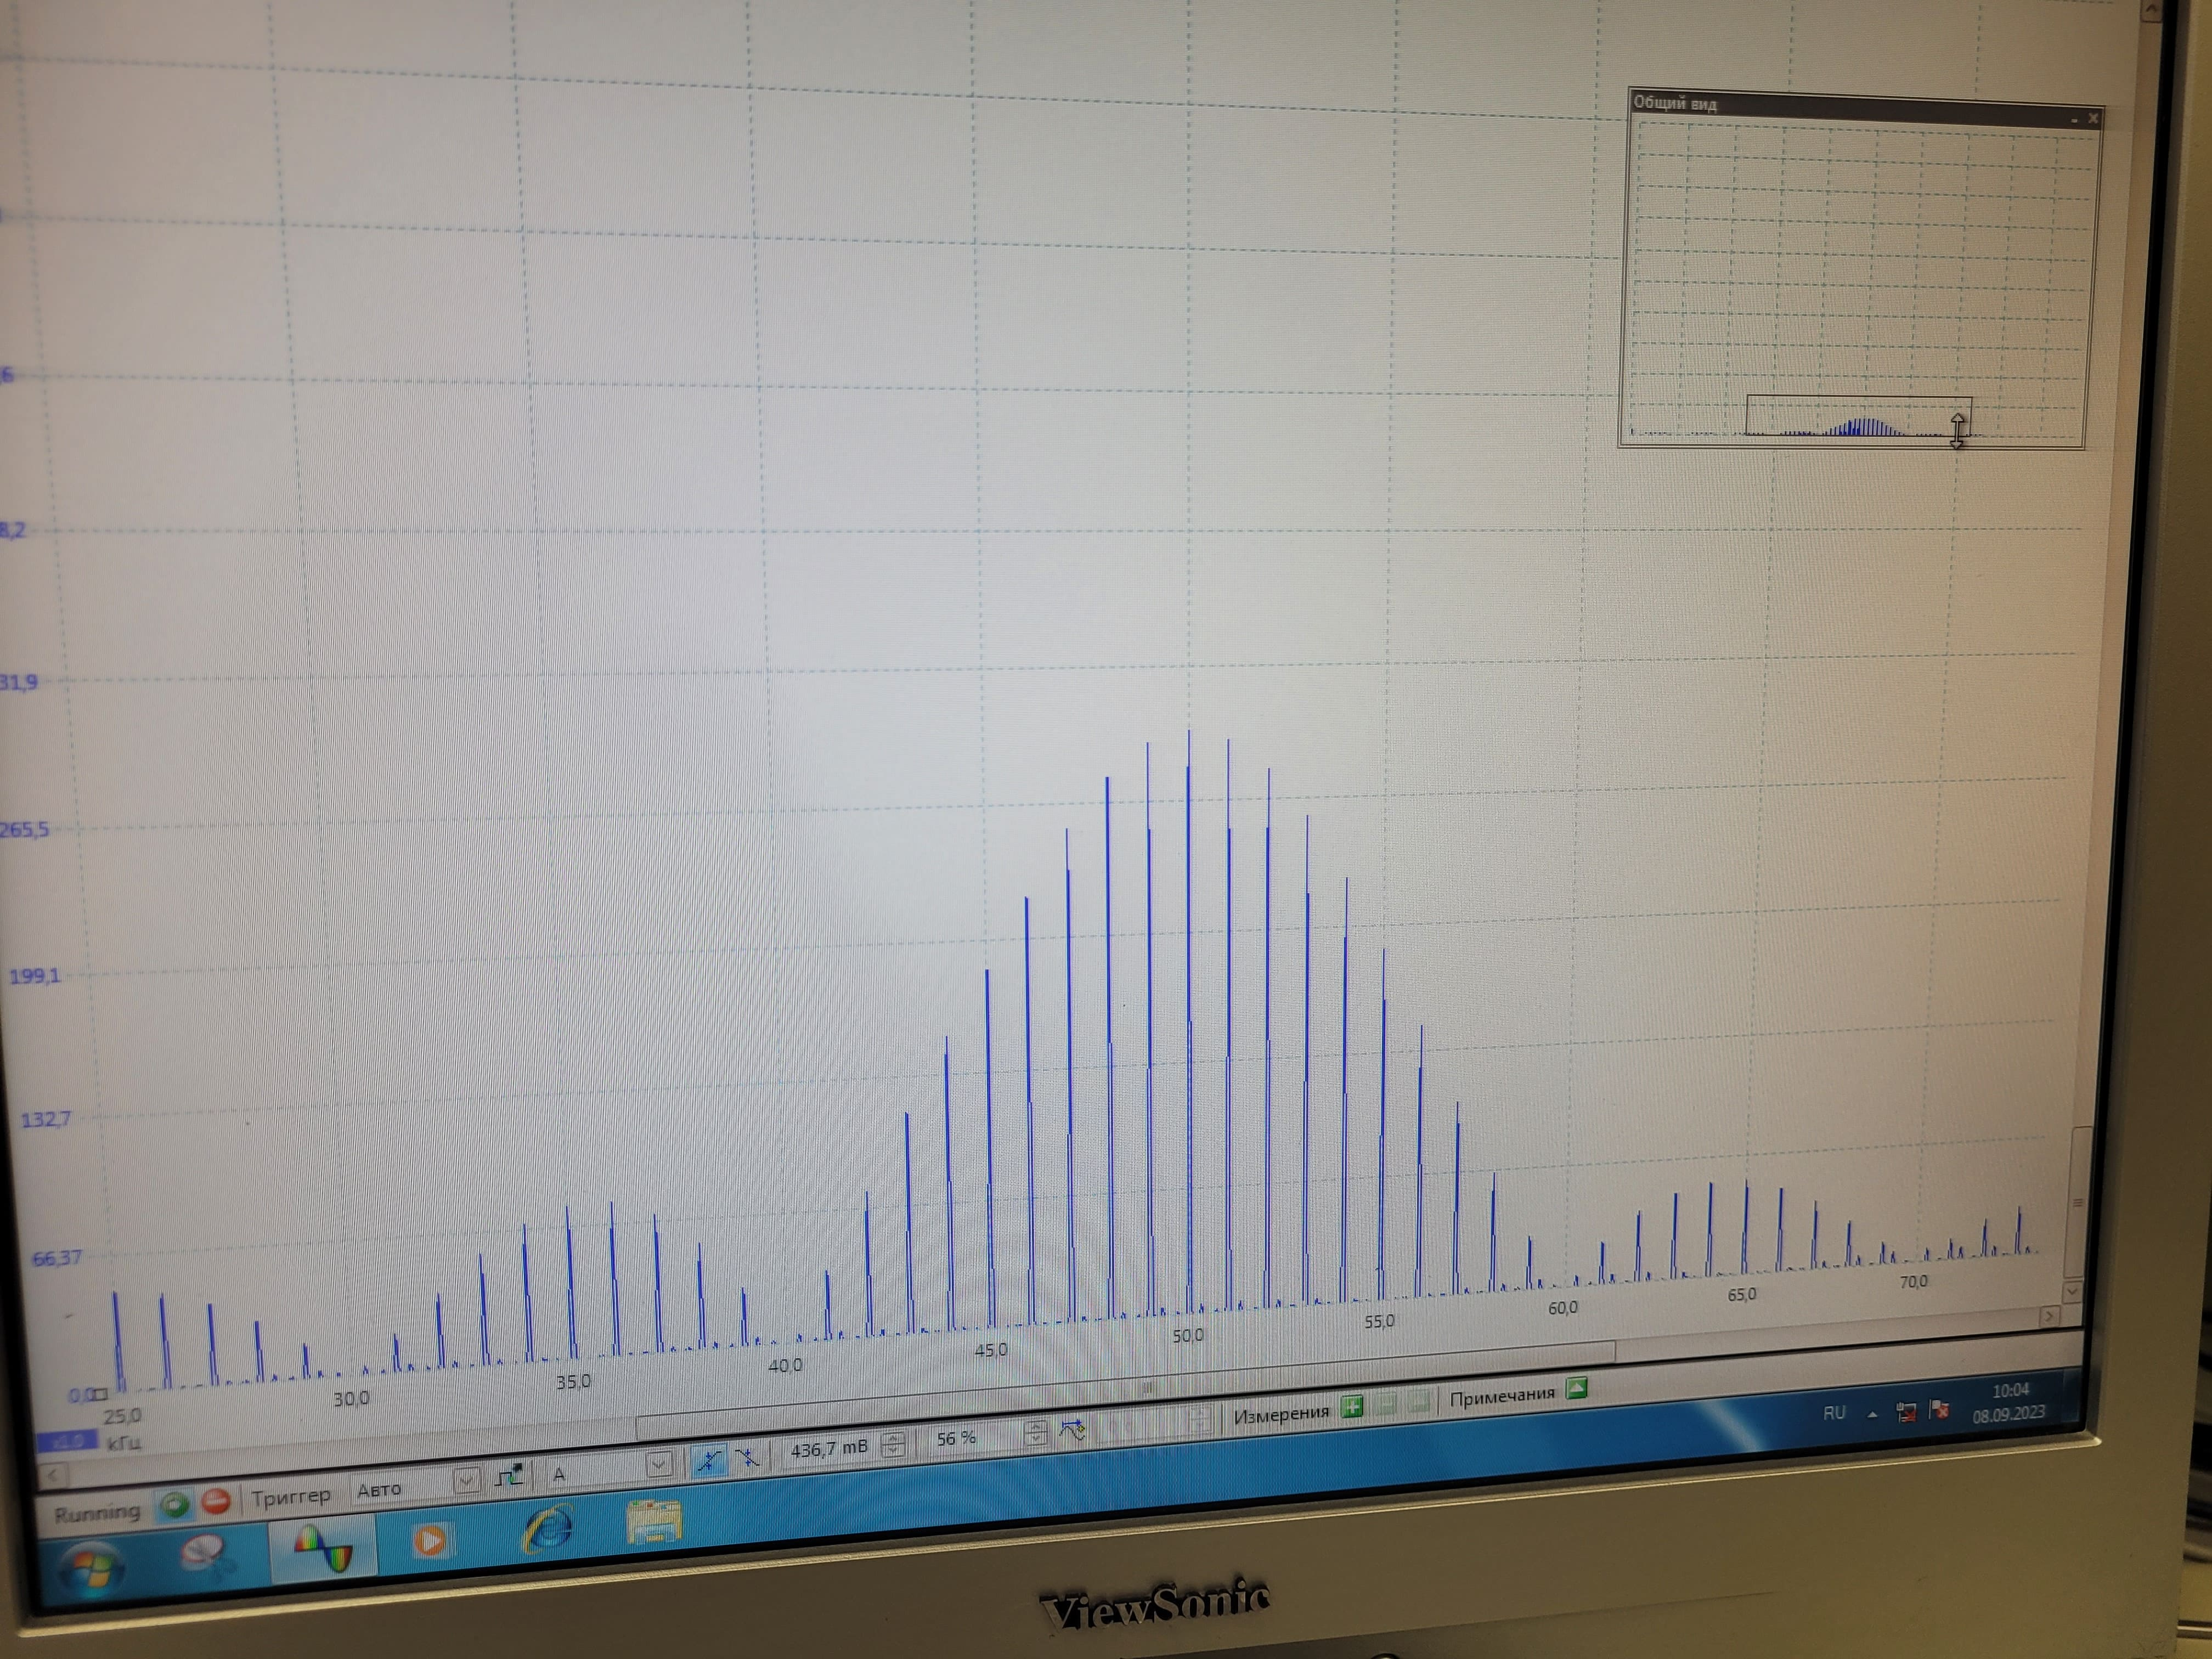
\includegraphics[width=1\linewidth]{B_50k_1k_5.jpg}} N=5, $\delta \nu$ = 1 кГц, $\Delta \nu$ = 10 кГц\\
\end{minipage}
\hfill
\begin{minipage}[h]{0.47\linewidth}
\center{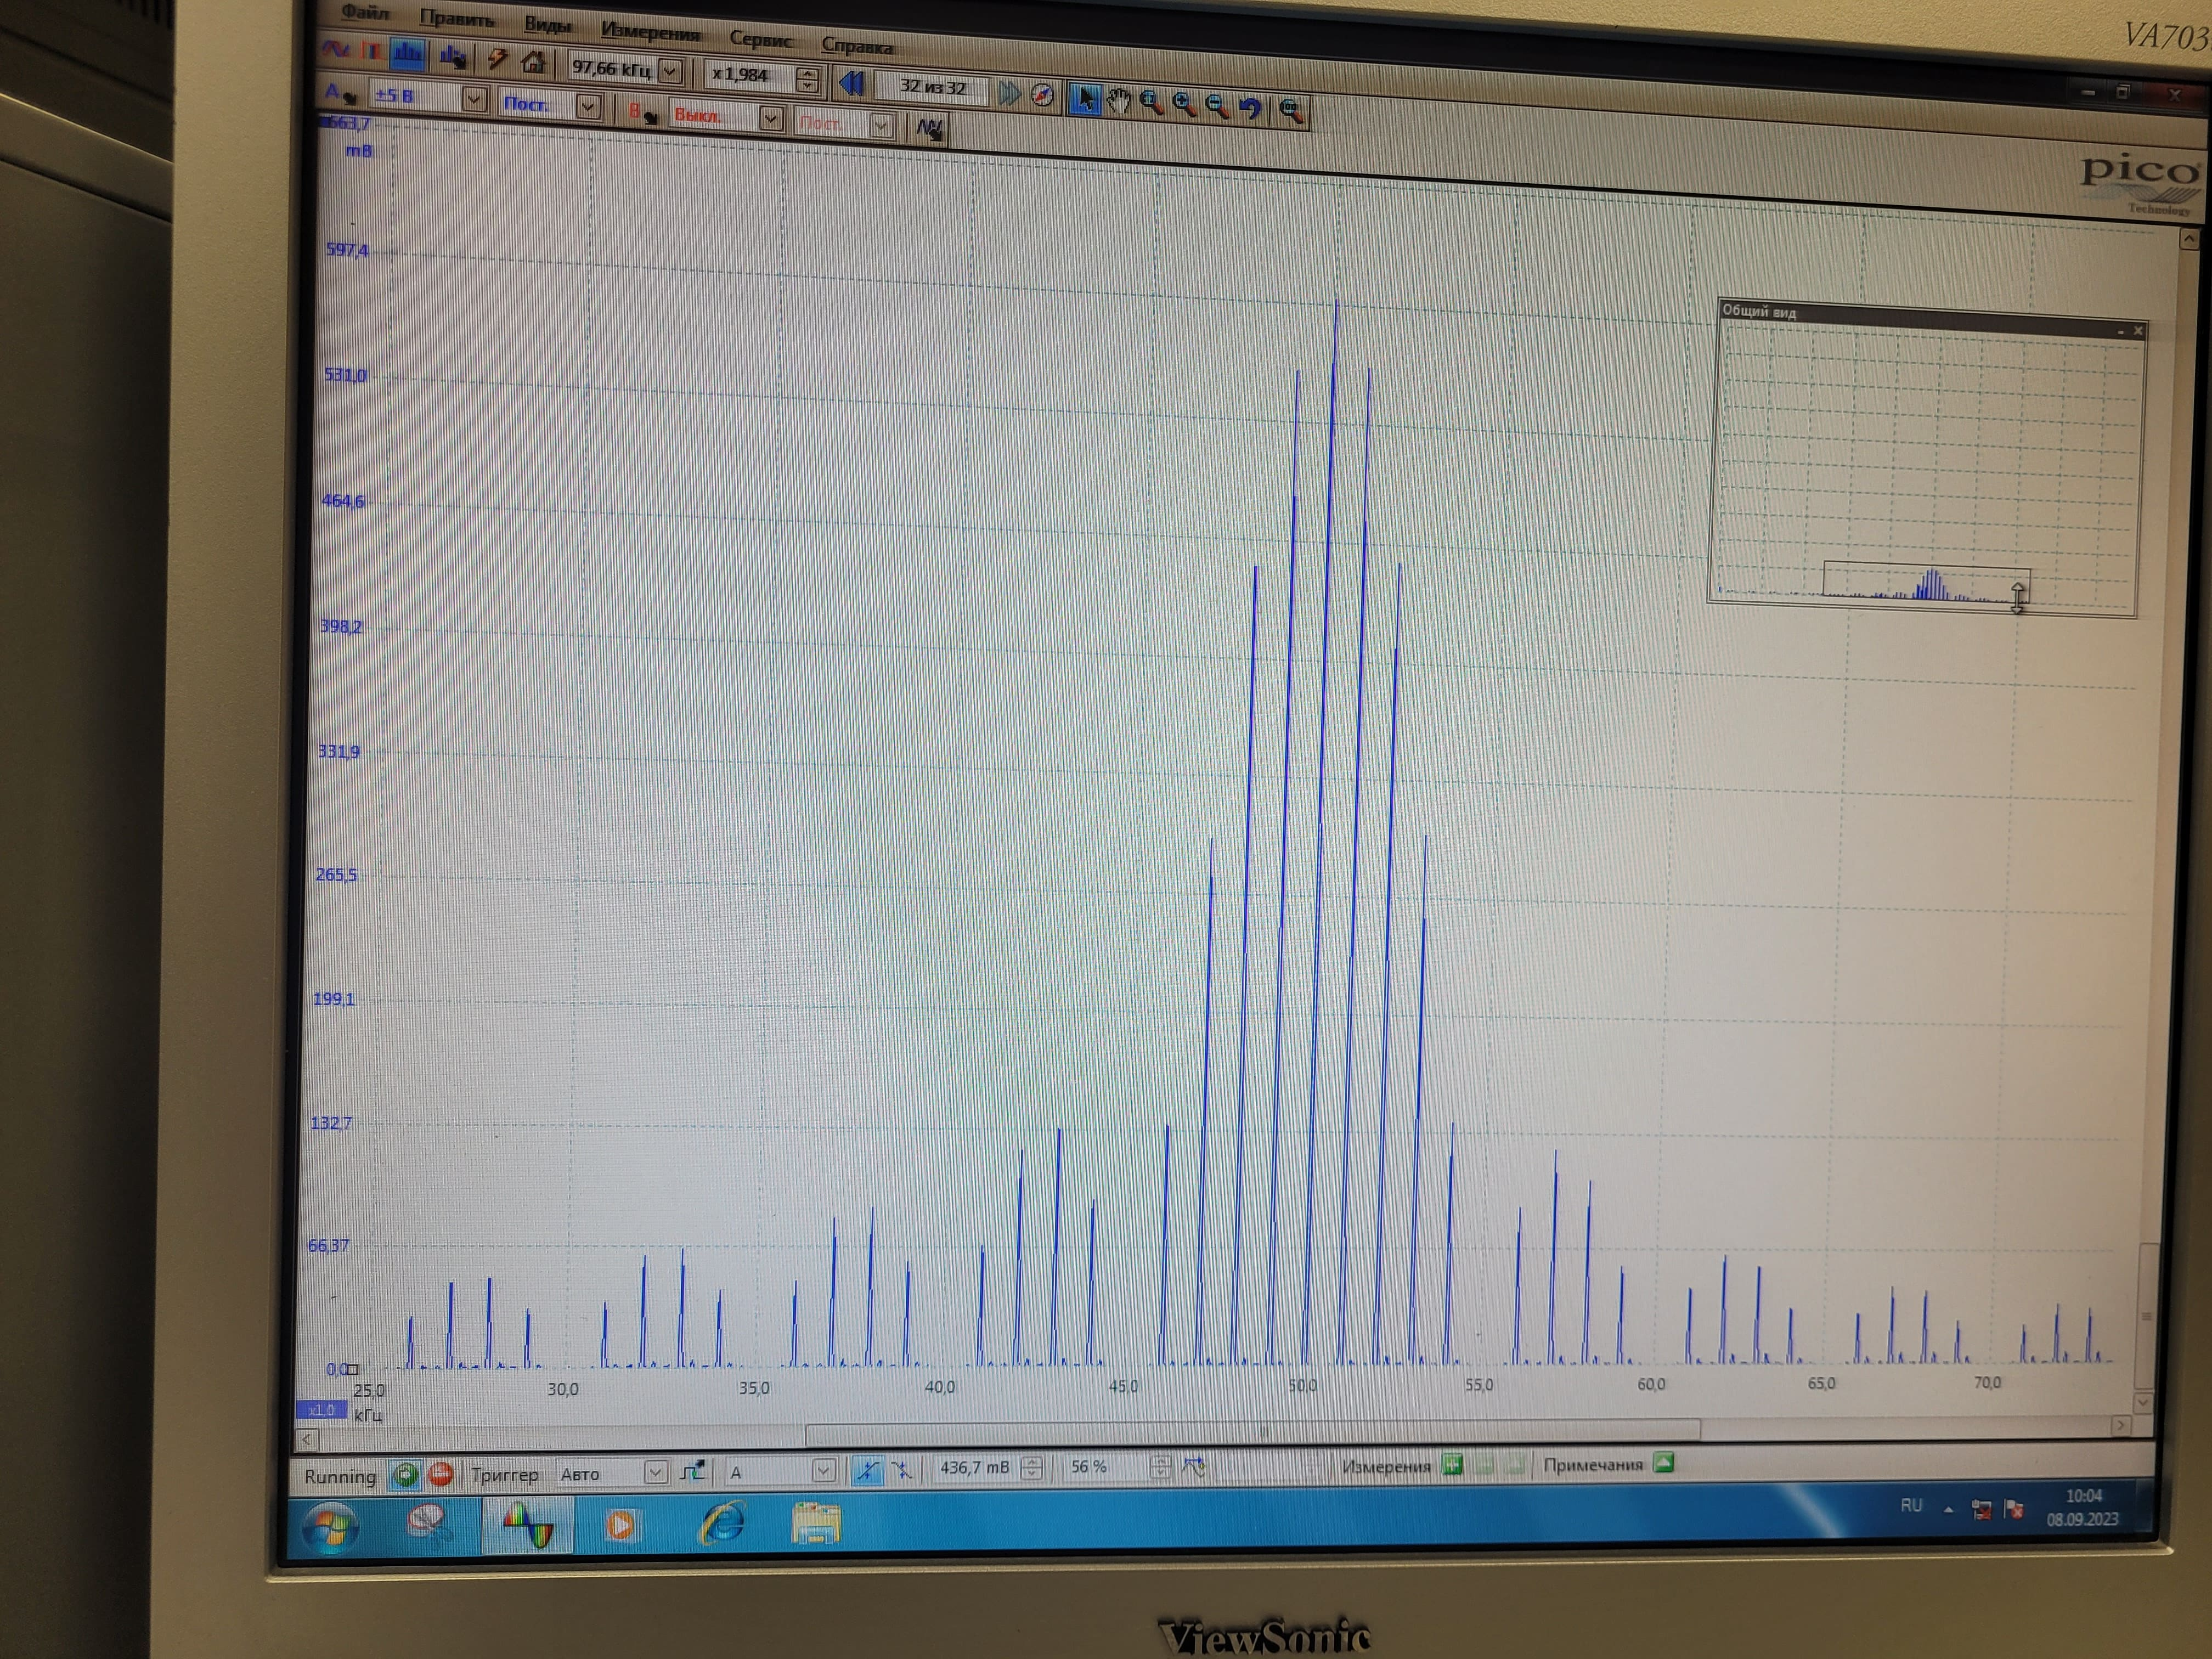
\includegraphics[width=1\linewidth]{B_50k_1k_10.jpg}} \\N=10, $\delta \nu$ = 1 кГц, $\Delta \nu$ = 5 кГц
\end{minipage}
\vfill
\begin{minipage}[h]{0.47\linewidth}
\center{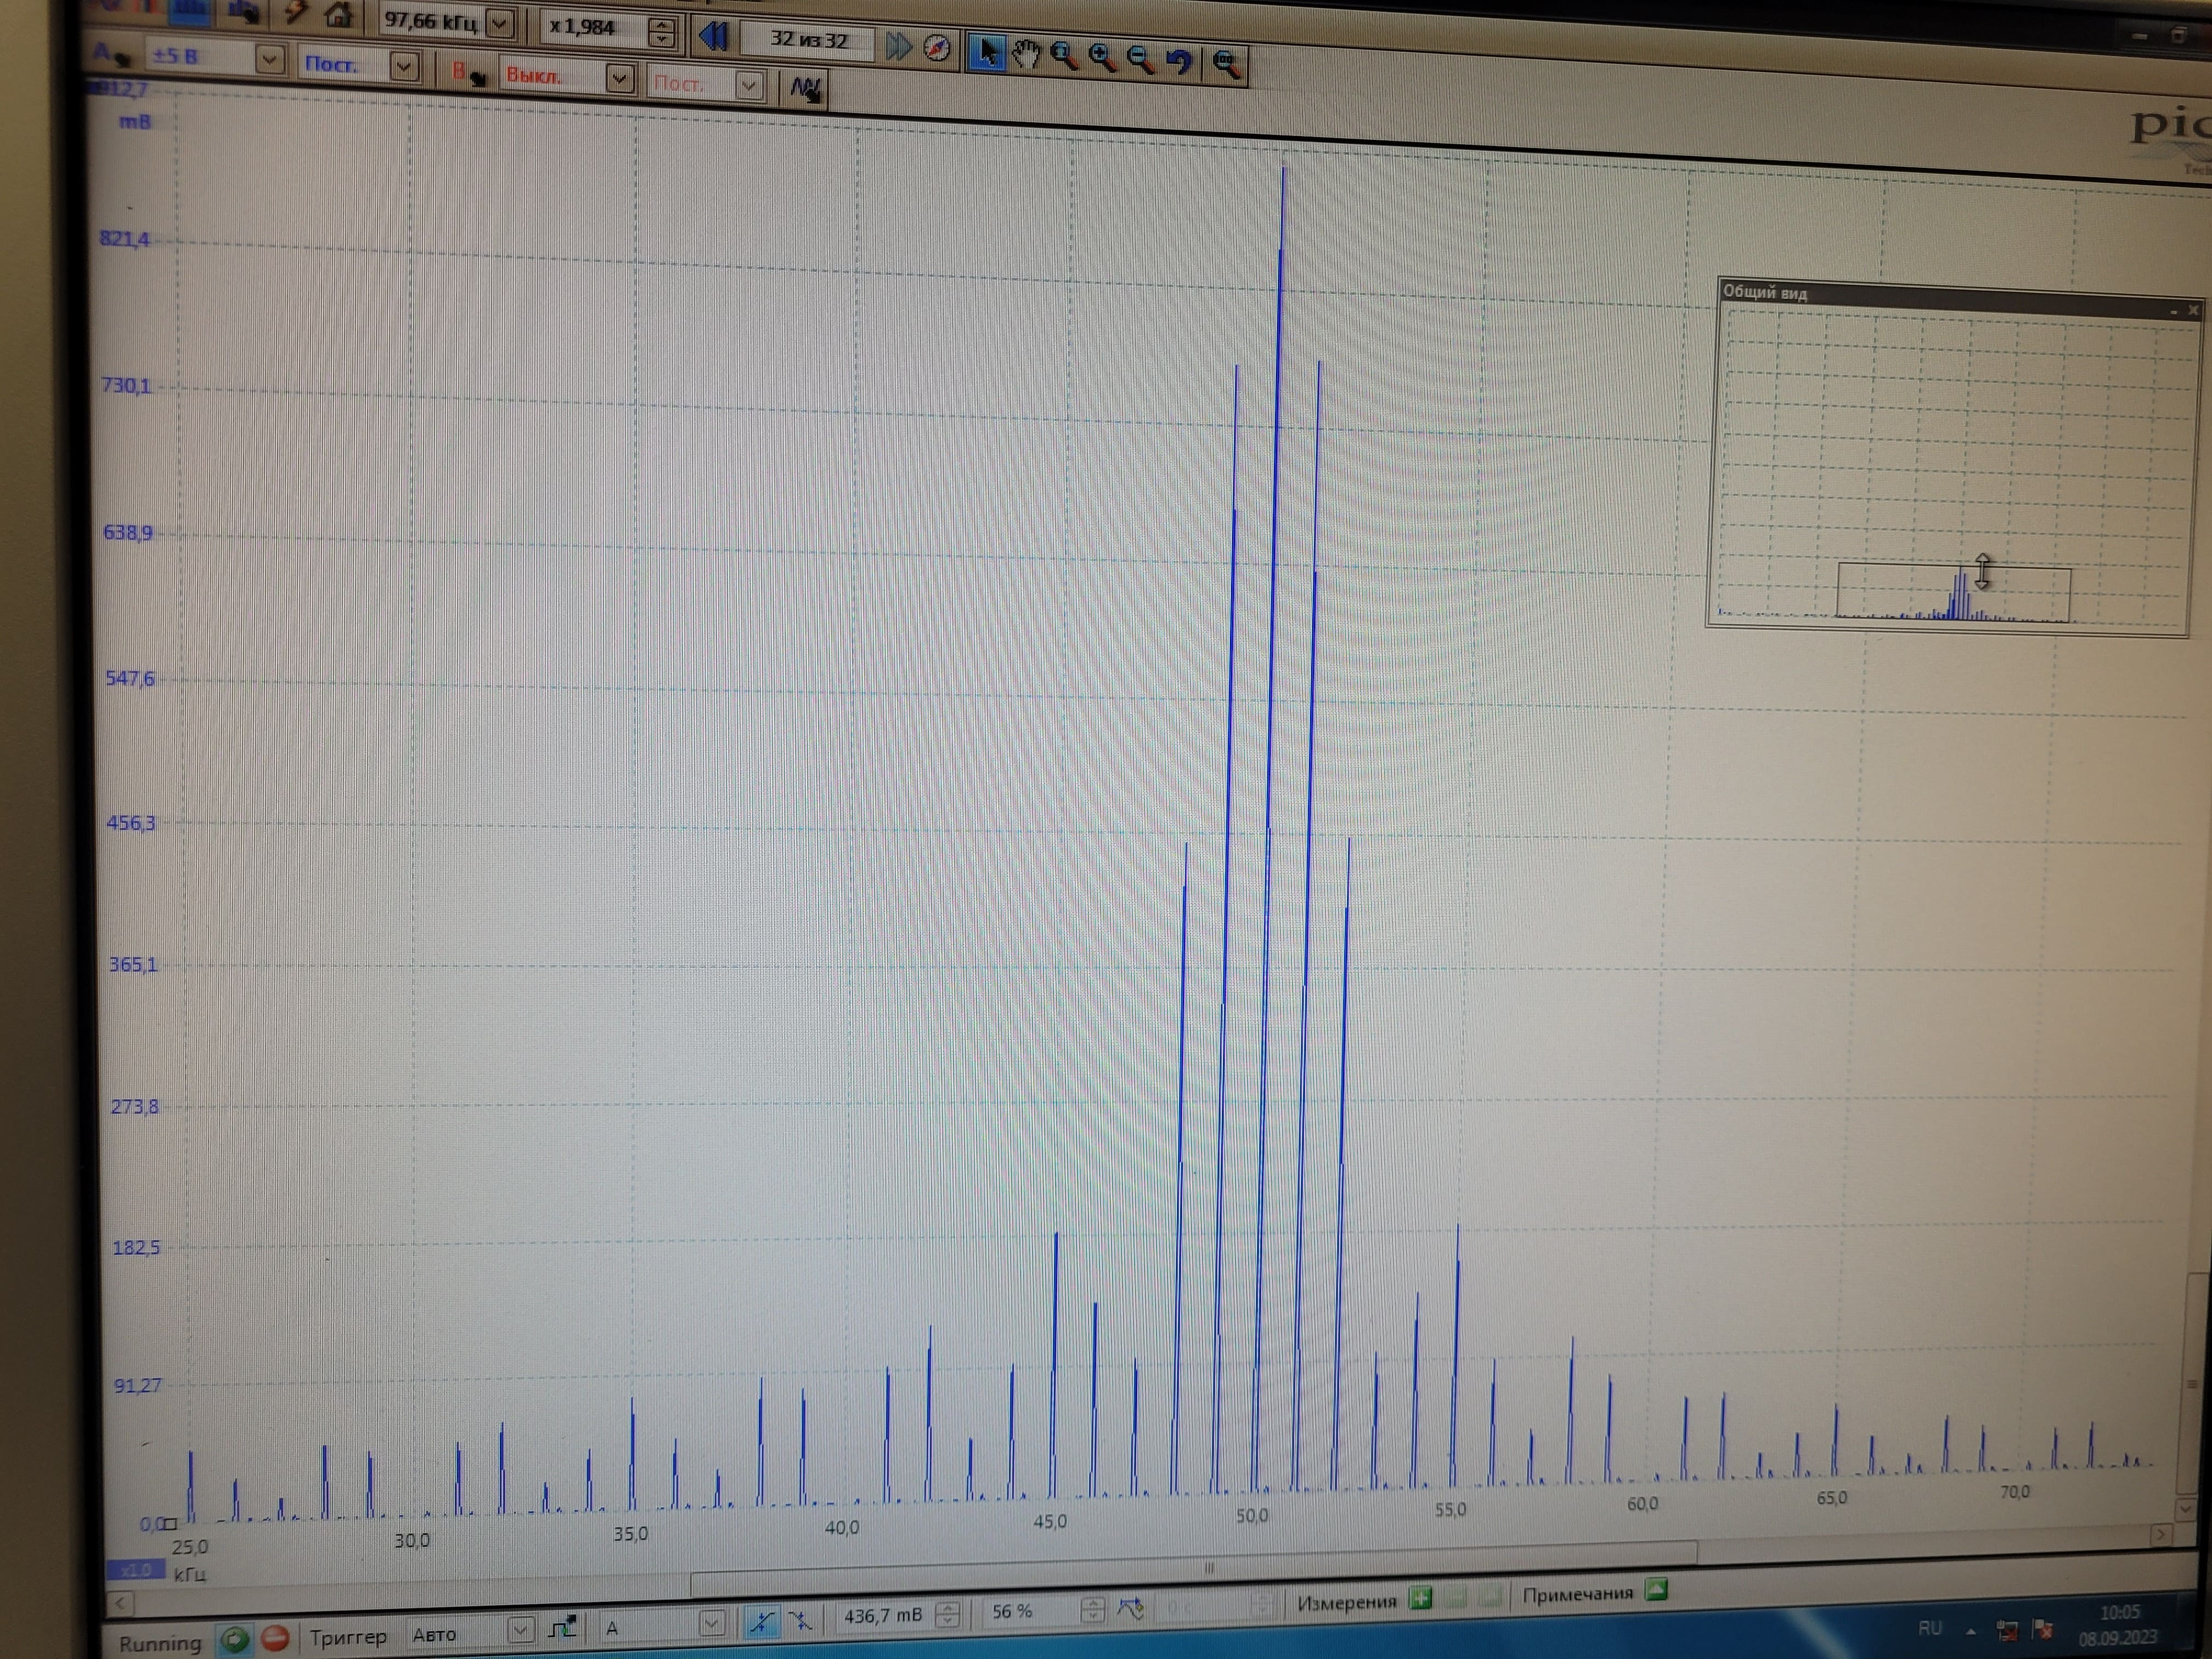
\includegraphics[width=1\linewidth]{B_50k_1k_15.jpg}} N=15, $\delta \nu$ = 1 кГц, $\Delta \nu$ $\approx$ 3 кГц \\
\end{minipage}
\hfill
\begin{minipage}[h]{0.47\linewidth}
\center{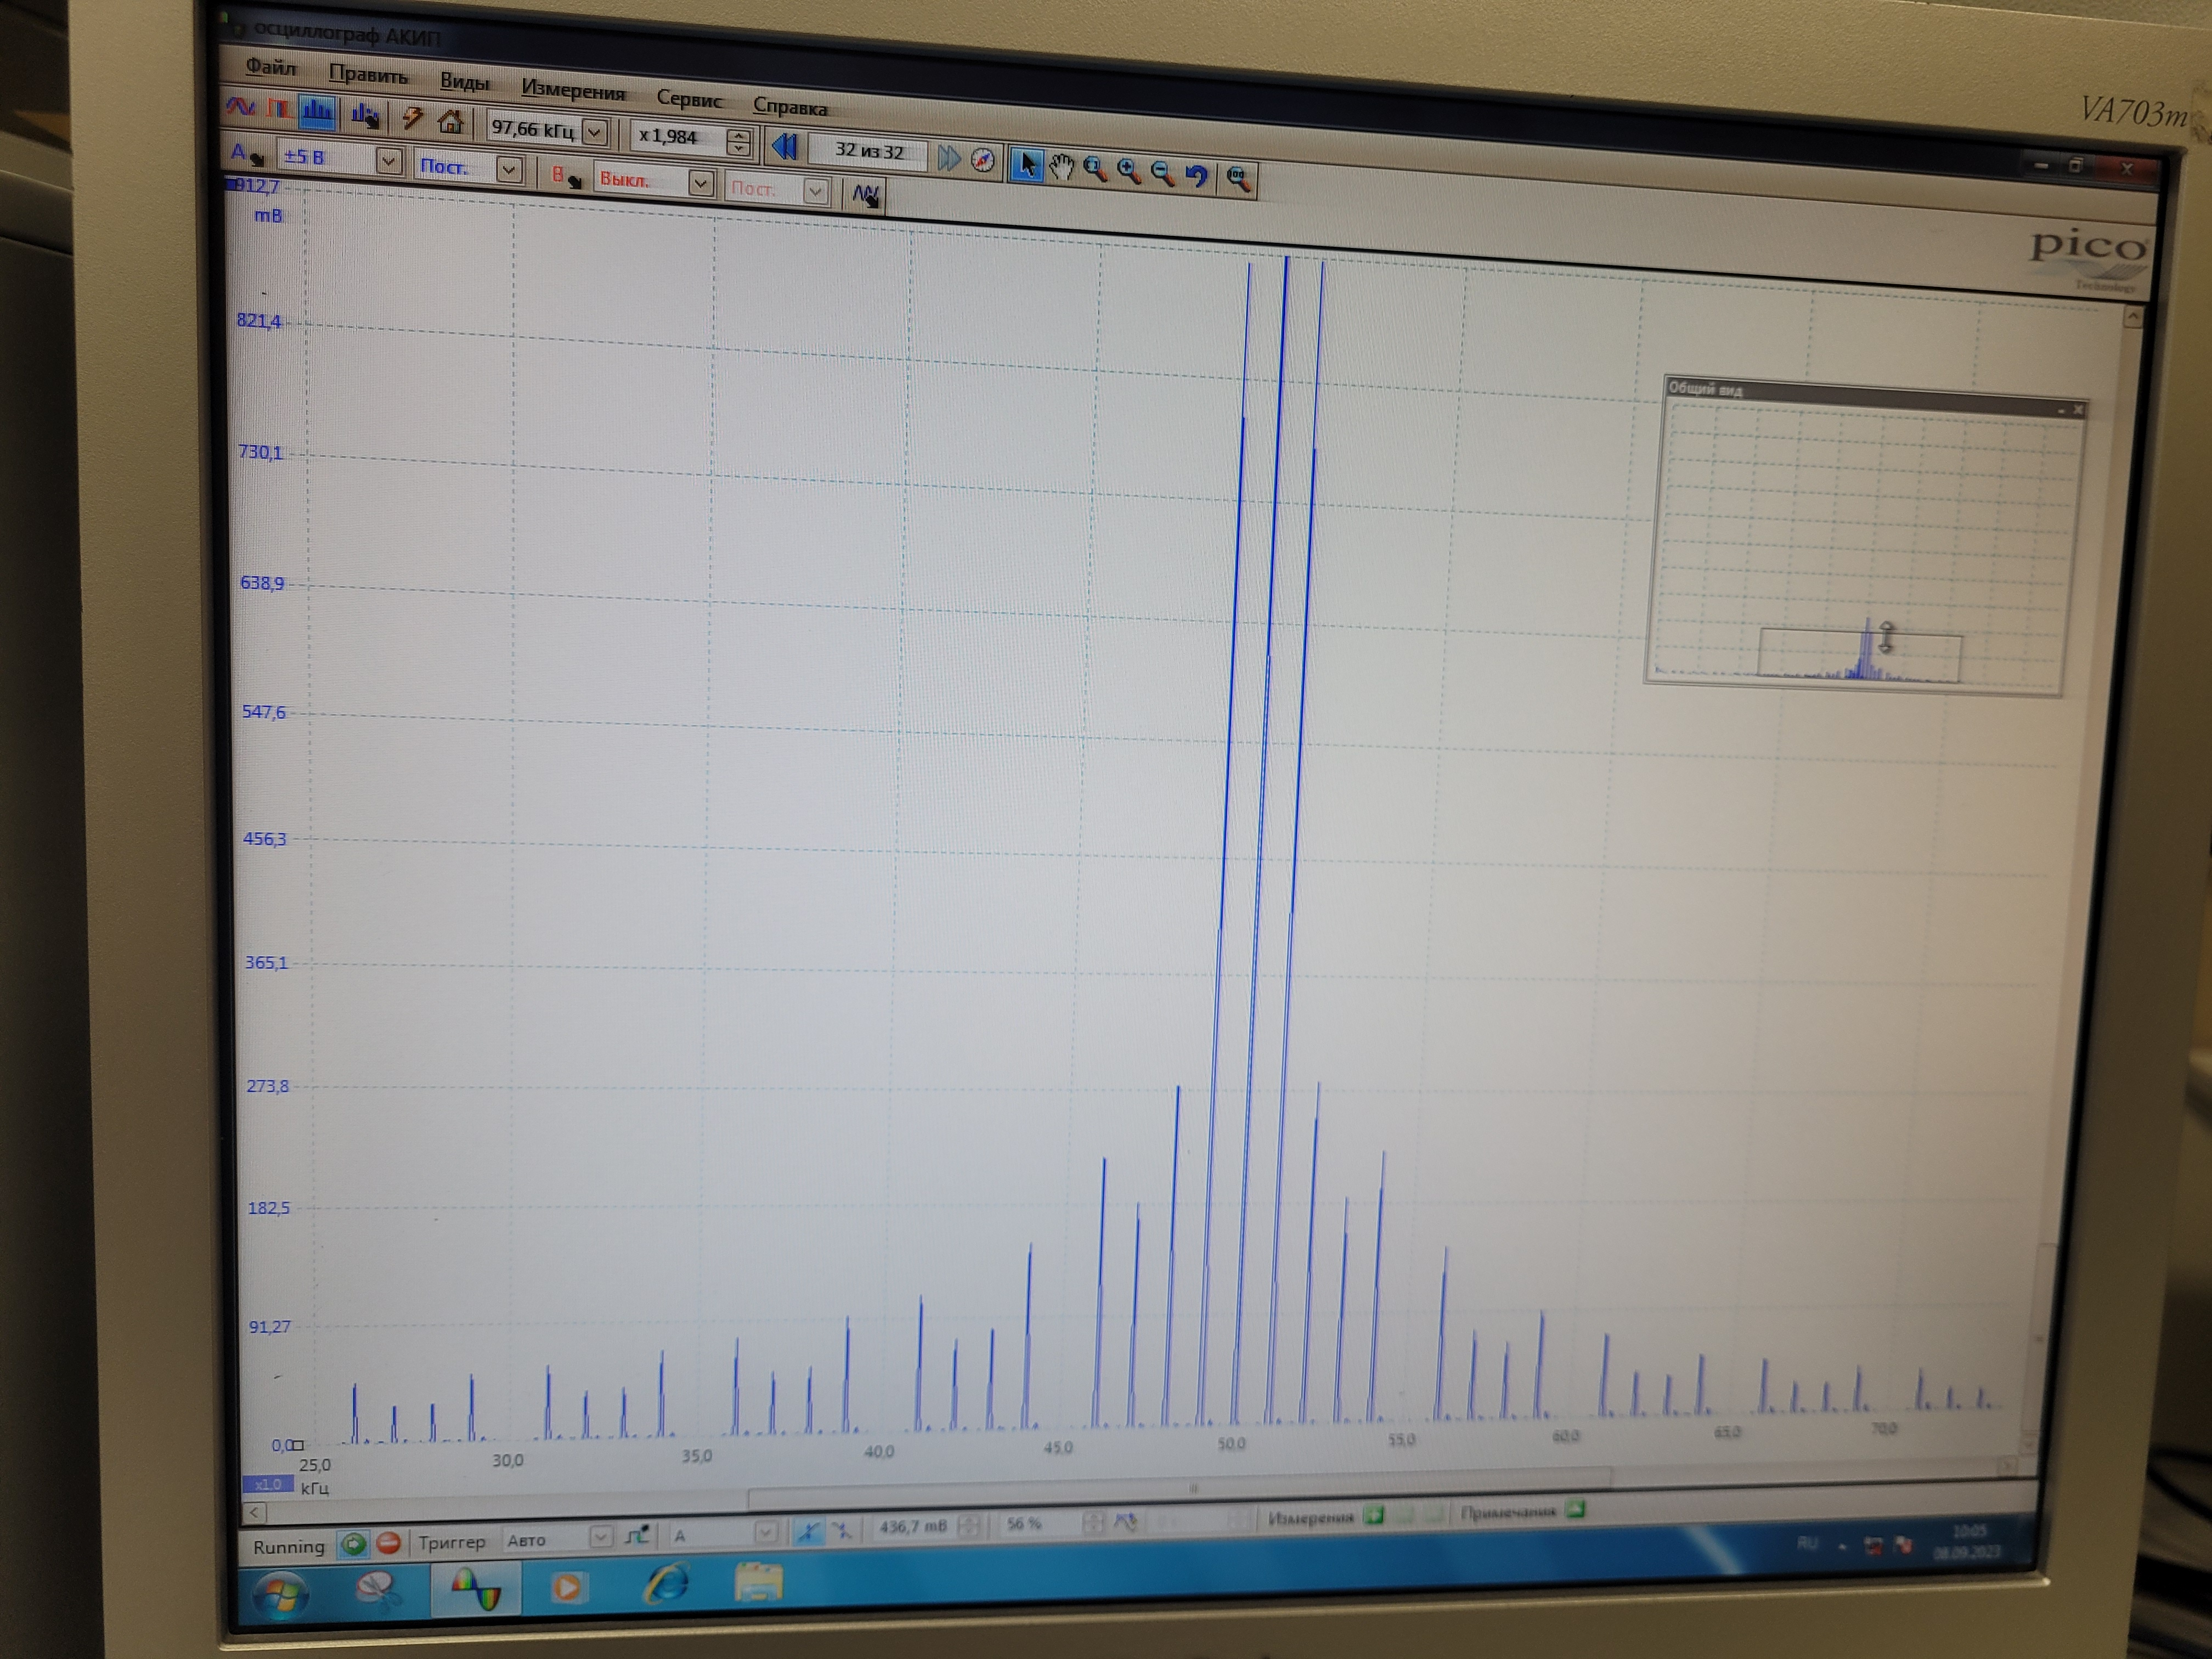
\includegraphics[width=1\linewidth]{B_50k_1k_20.jpg}} N=20, $\delta \nu$ = 1 кГц, $\Delta \nu$ $\approx$ 2.5 кГц \\
\end{minipage}
\caption{}
\label{ris:experimentalcorrelationsignals}
\end{figure}

Соотношение неопределённостей:
$$ \Delta \nu \cdot \tau = 10\cdot10^3\frac{5}{50\cdot10^3} = 5\cdot10^3\frac{10}{50\cdot10^3} = 2.5\cdot10^3\frac{20}{50\cdot10^3} \approx 3\cdot10^3\frac{15}{50\cdot10^3} \approx 1 $$\\

Видим, что спектр остаётся симметричным относительно одной и той же точки, однако "сжимается" к ней при увеличении N.


\newpage

\textbf{б.} Изменяем $\nu_0$ при фиксированных N = 5 и $\nu_\text{повт}$ = 1 кГц:

\begin{figure}[h]
\begin{minipage}[h]{0.47\linewidth}
\center{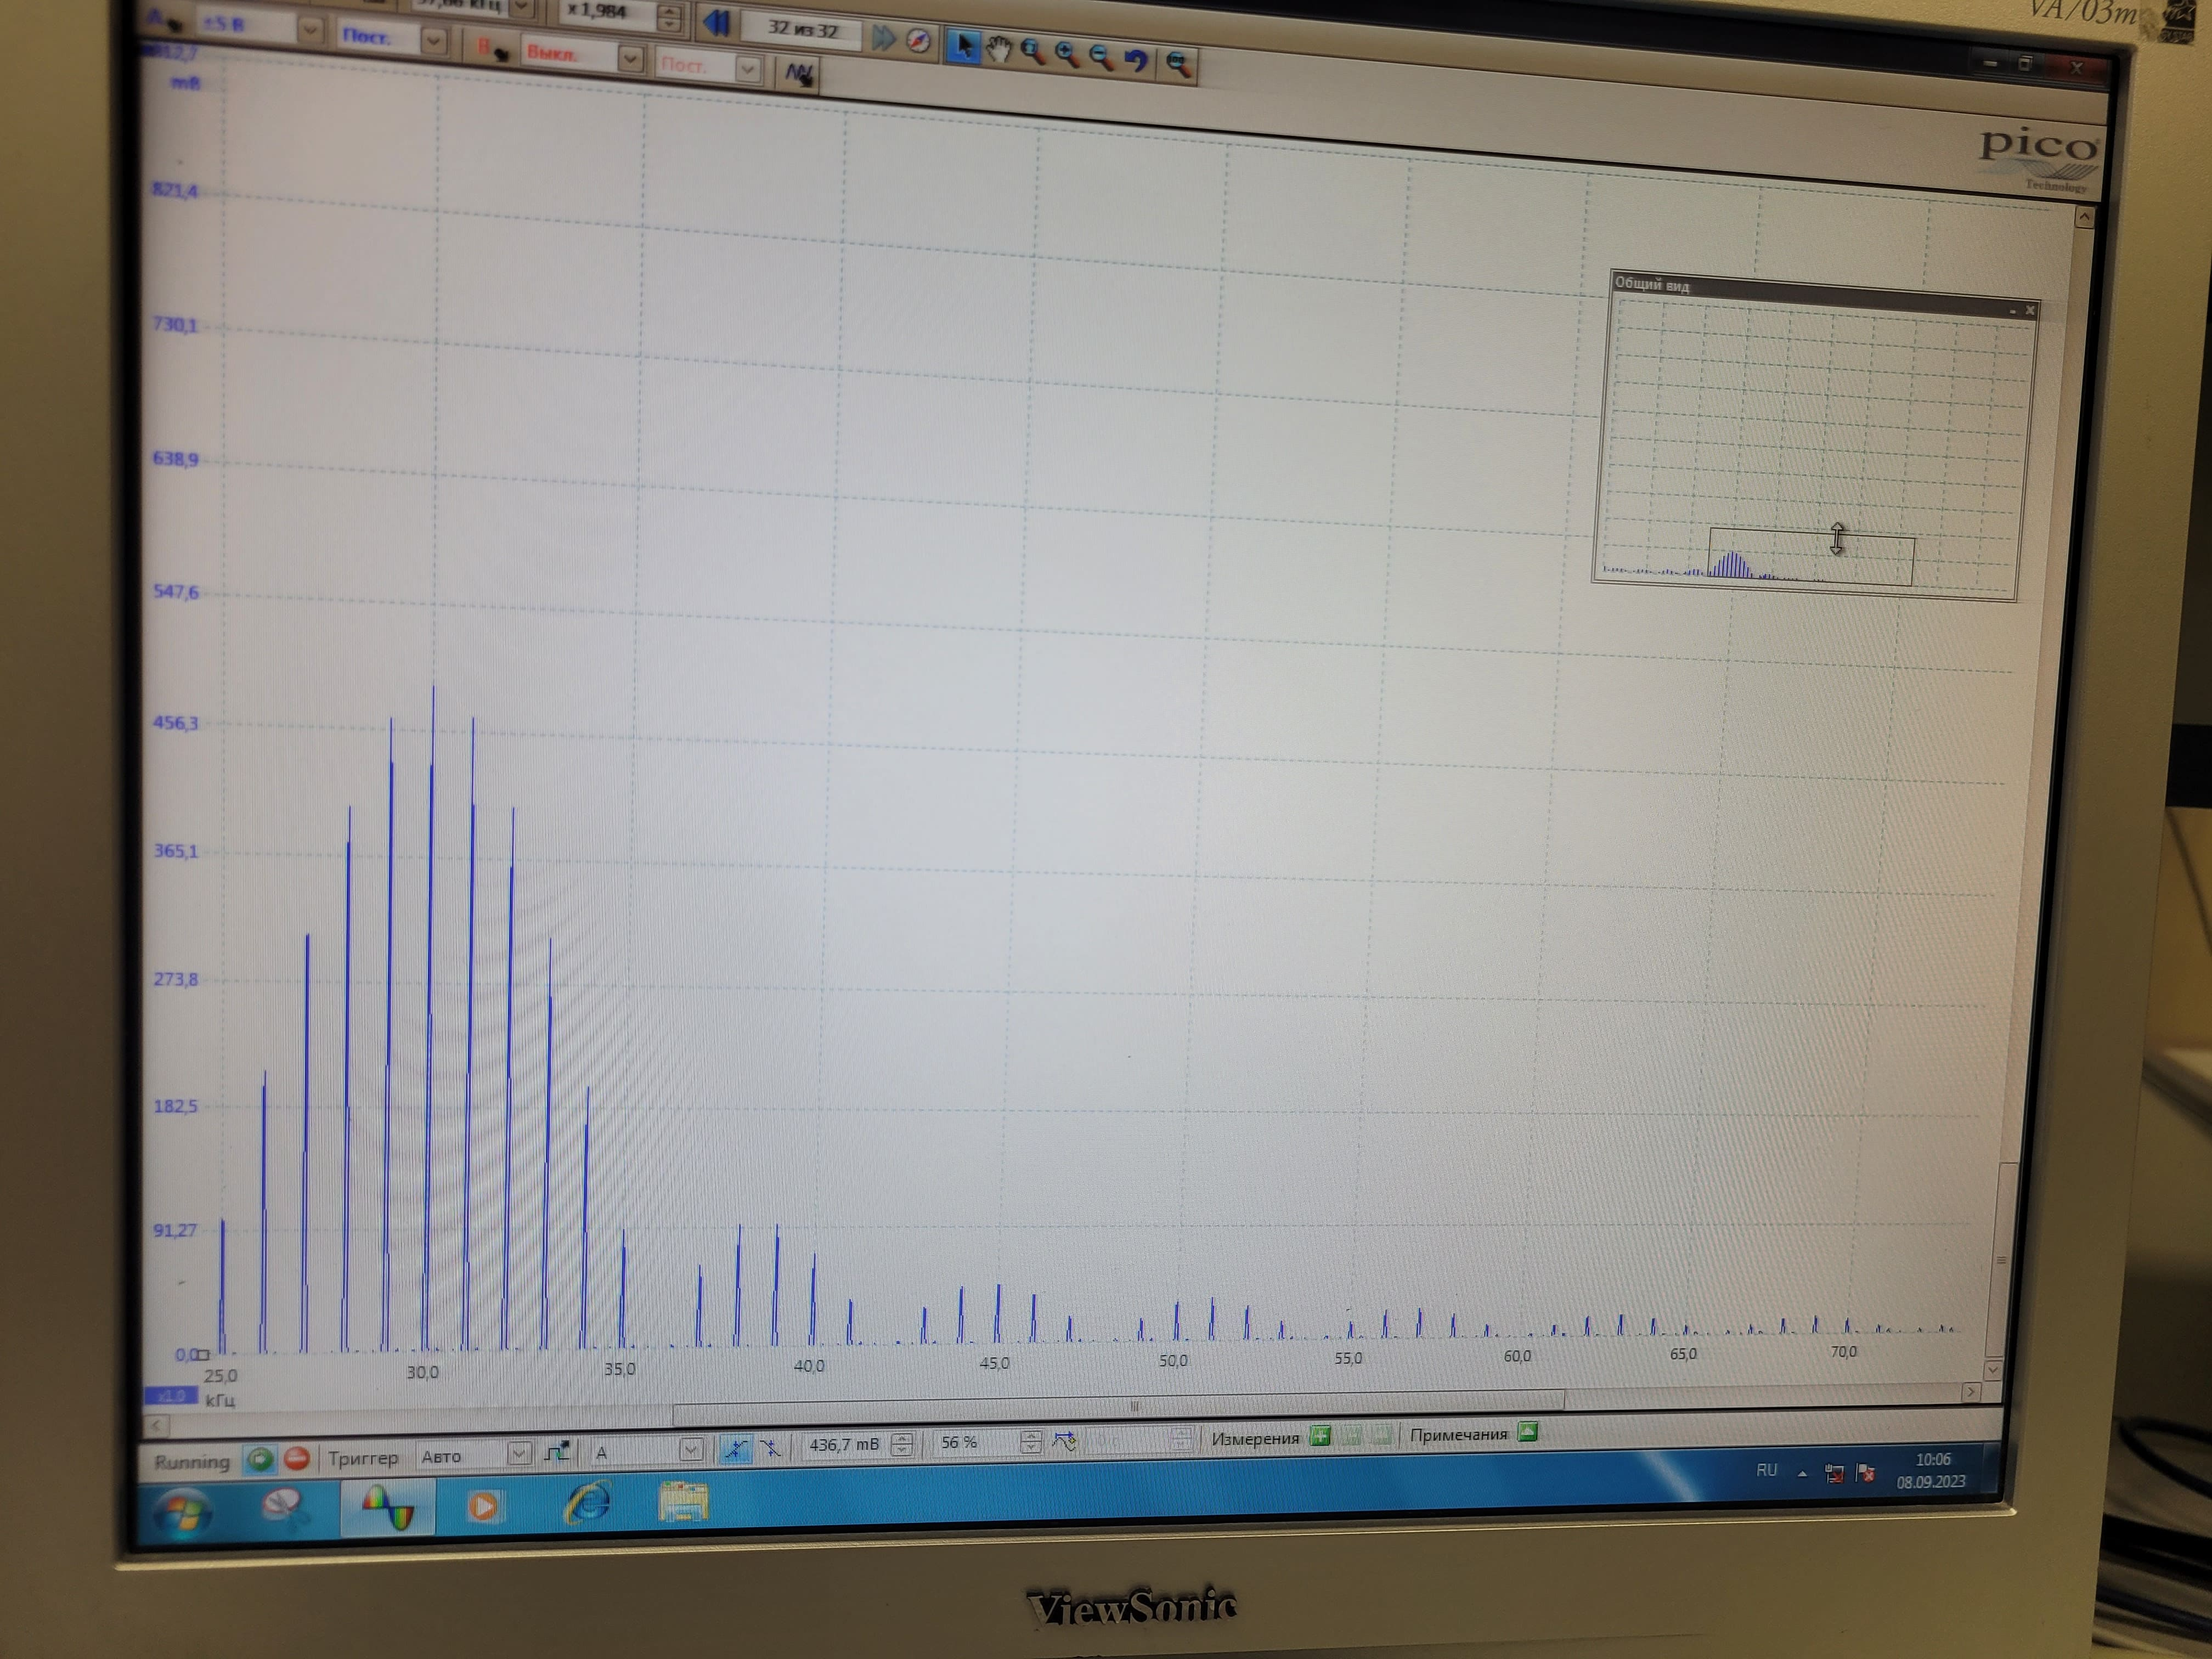
\includegraphics[width=1\linewidth]{B_30k_1k_5.jpg}} $\nu_0$ = 30 кГц, $\delta \nu$ = 1 кГц, $\Delta \nu$ = 6 кГц  \\
\end{minipage}
\hfill
\begin{minipage}[h]{0.47\linewidth}
\center{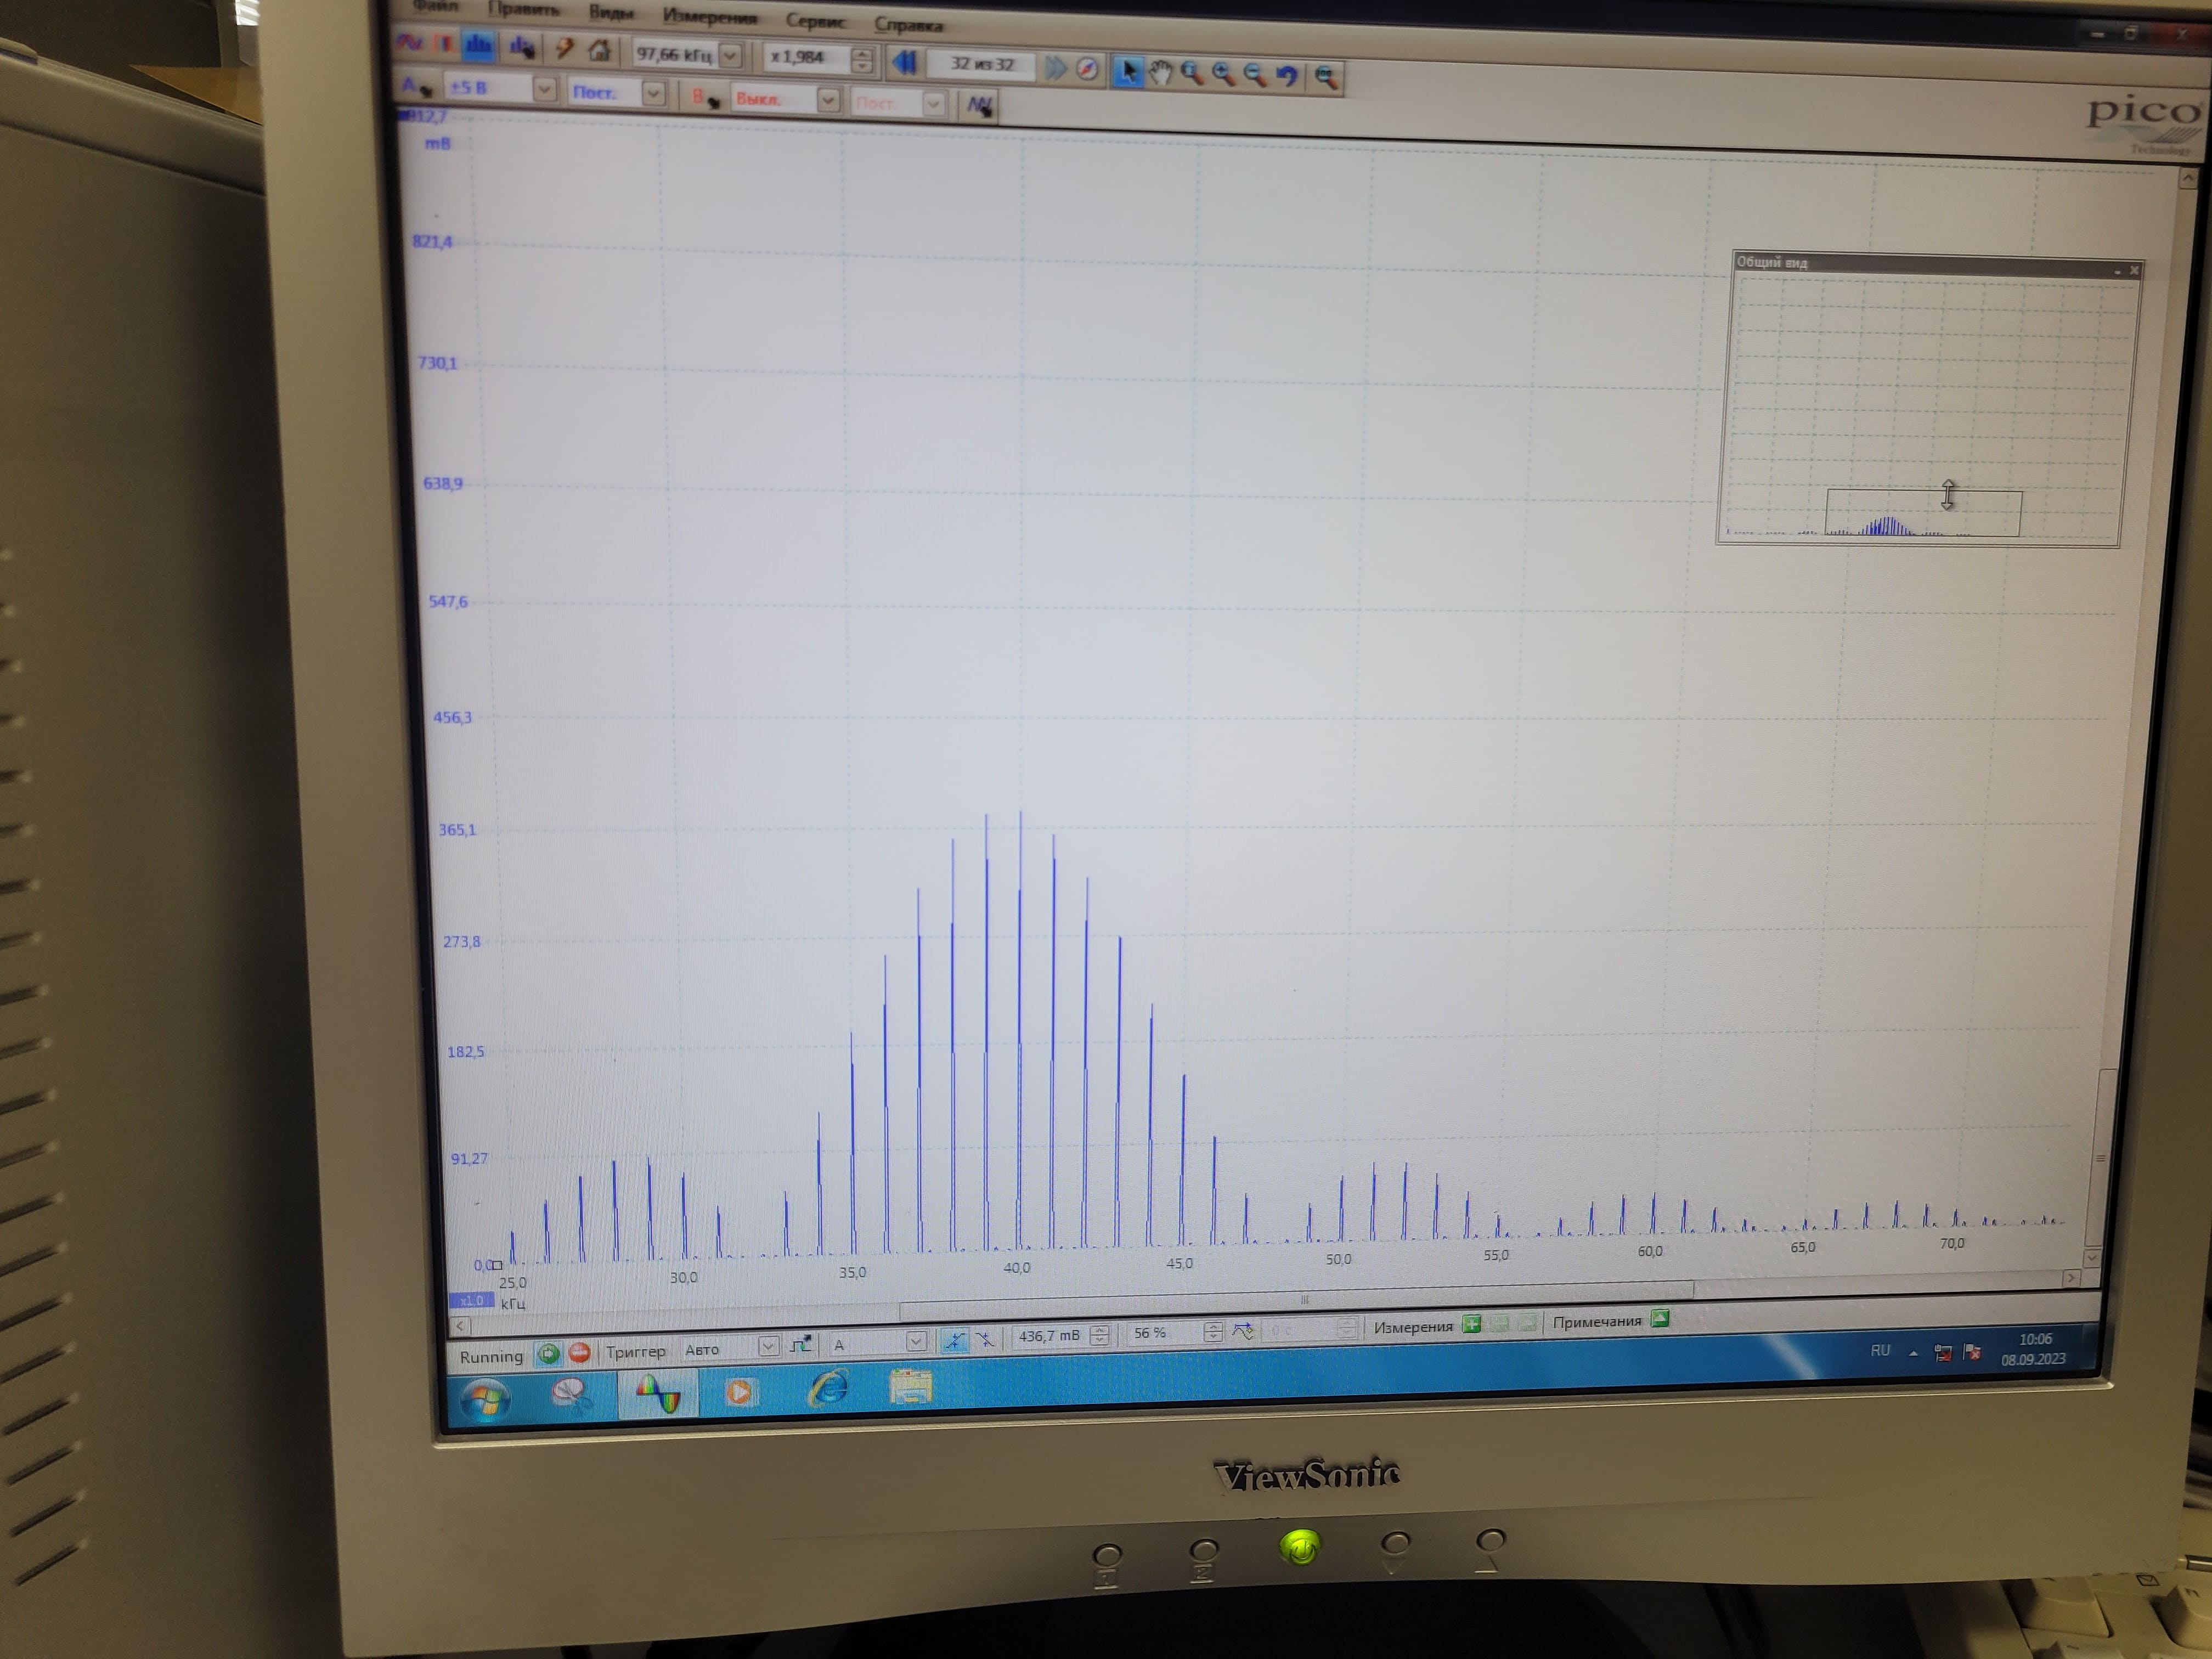
\includegraphics[width=1\linewidth]{B_40k_1k_5.jpg}} \\ $\nu_0$ = 40 кГц, $\delta \nu$ = 1 кГц, $\Delta \nu$ = 8 кГц
\end{minipage}
\vfill
\begin{minipage}[h]{0.47\linewidth}
\center{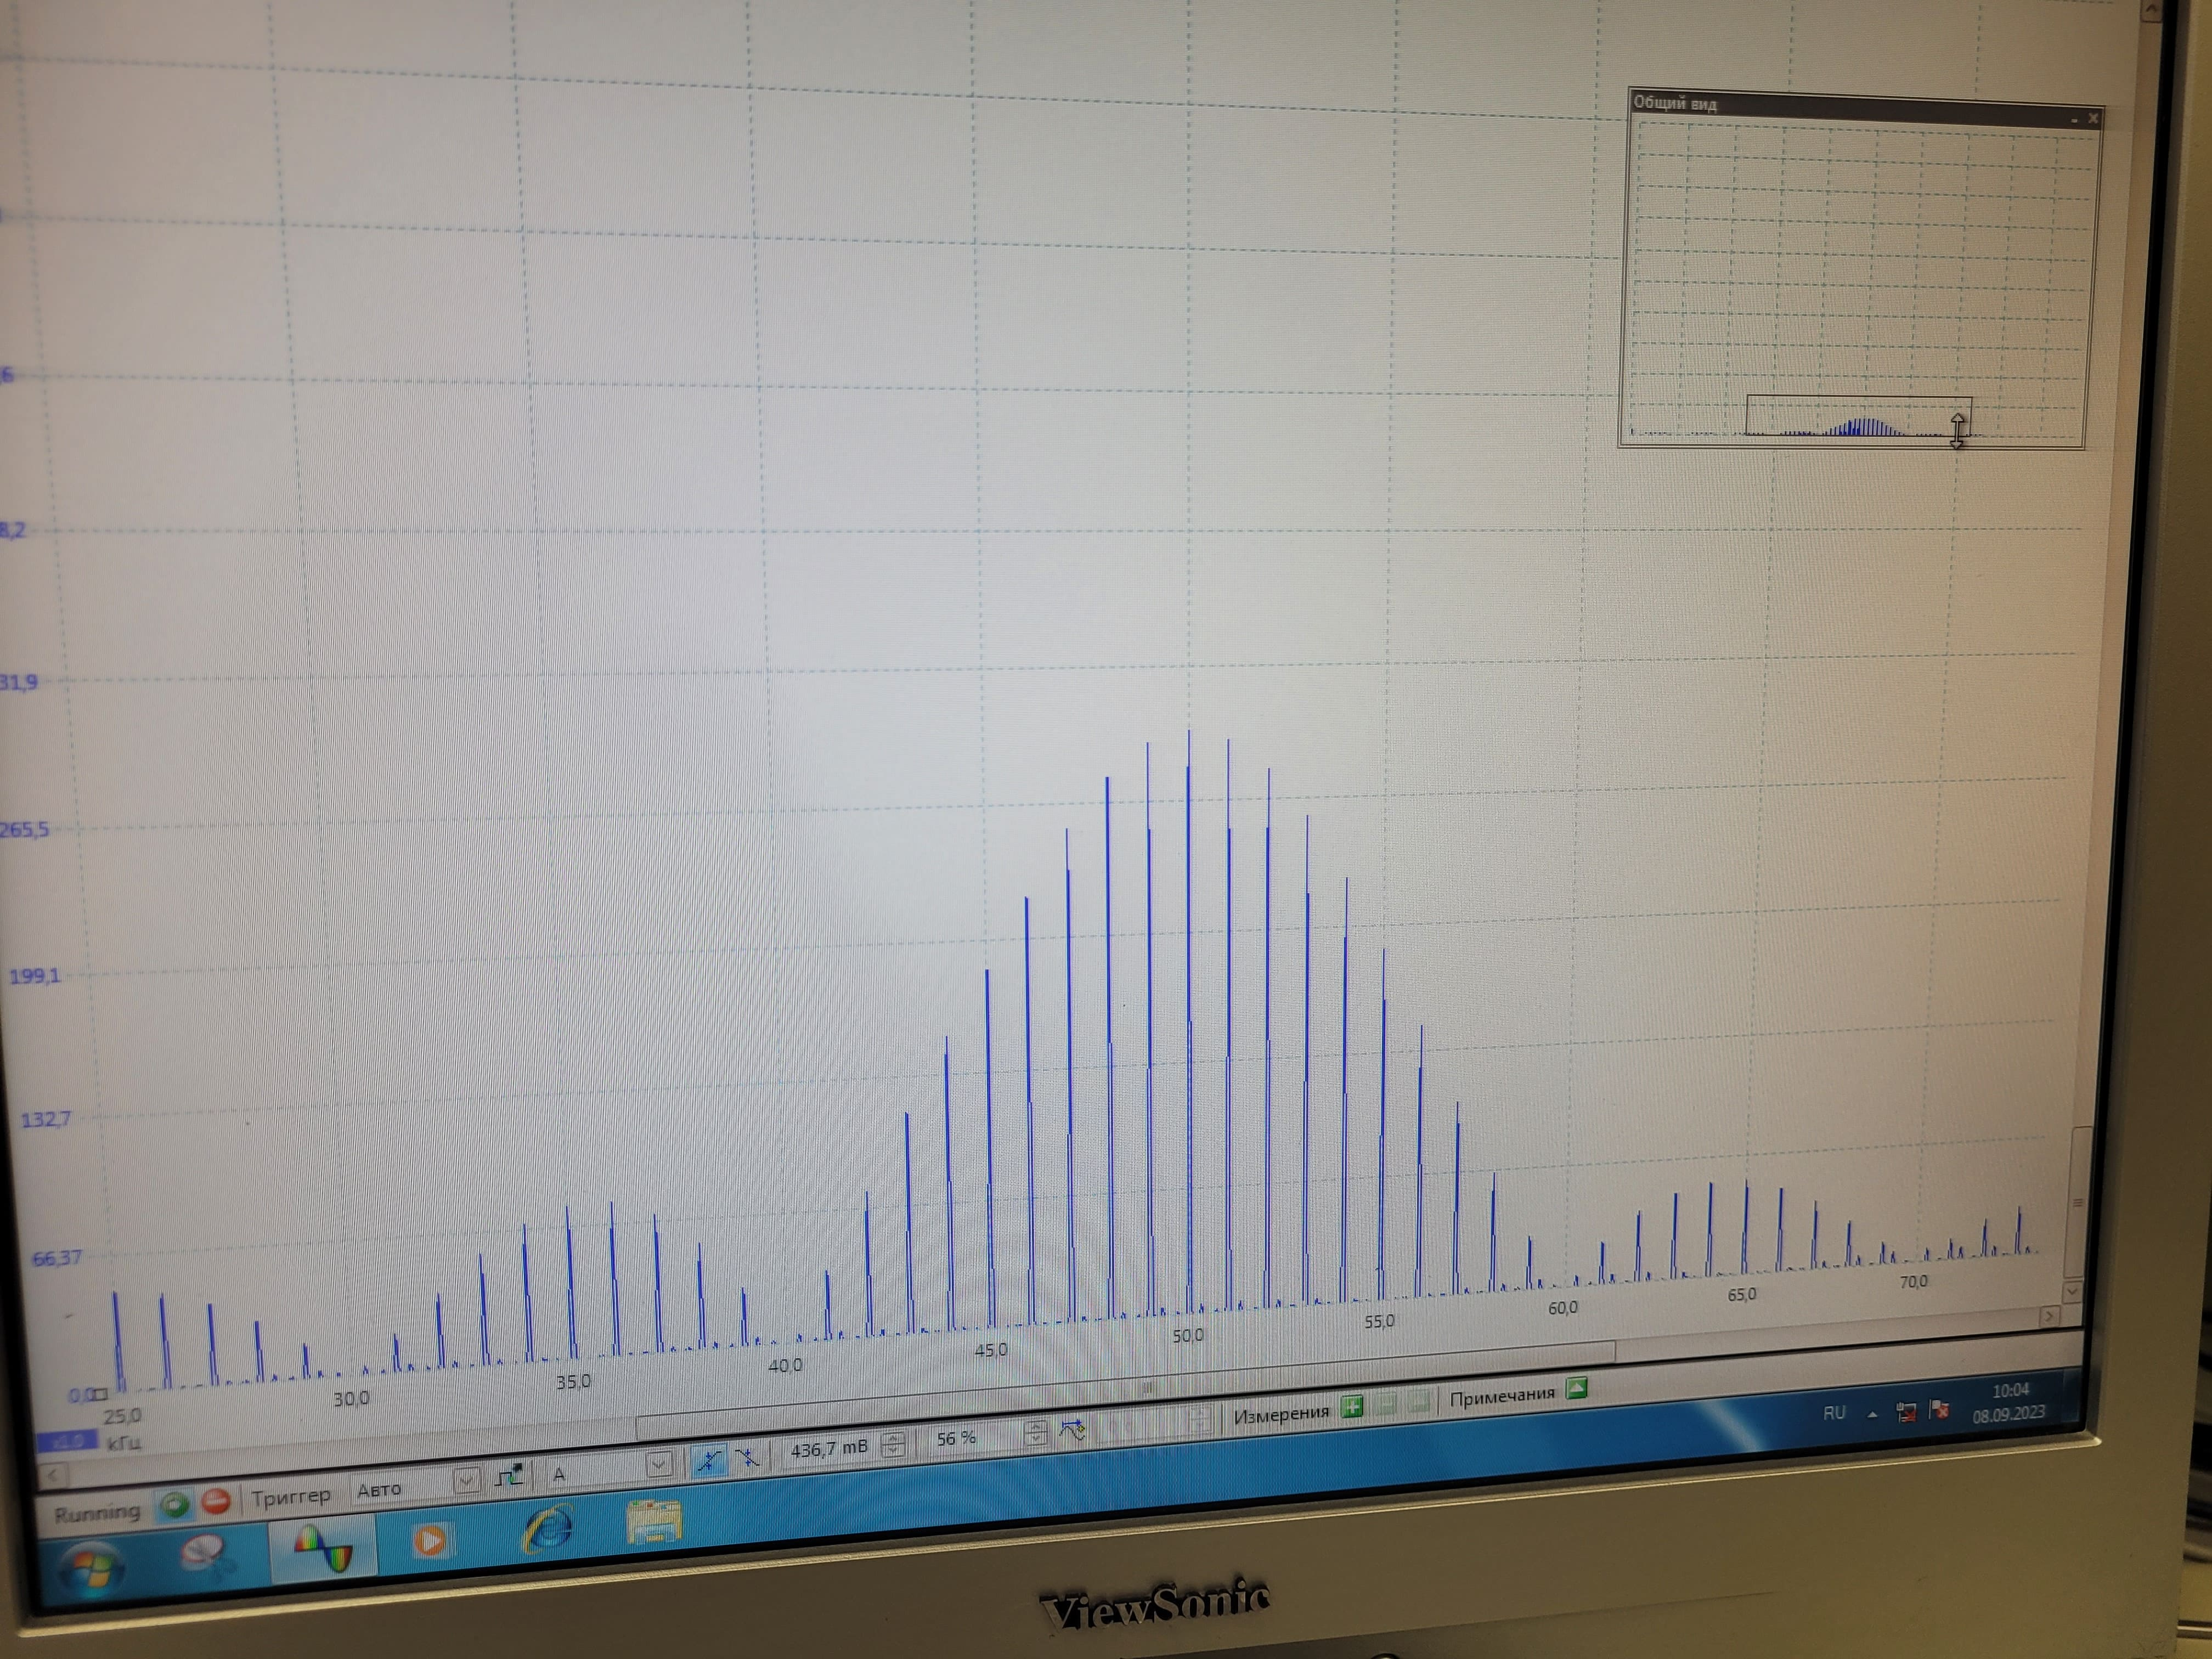
\includegraphics[width=1\linewidth]{B_50k_1k_5.jpg}} $\nu_0$ = 50 кГц, $\delta \nu$ = 1 кГц, $\Delta \nu$ = 10 кГц \\
\end{minipage}
\hfill
\caption{}
\label{ris:experimentalcorrelationsignals}
\end{figure}

Соотношение неопределённостей:
$$ \Delta \nu \cdot \tau = 6\cdot10^3\frac{5}{30\cdot10^3} = 8\cdot10^3\frac{5}{40\cdot10^3} = 10\cdot10^3\frac{5}{50\cdot10^3} = 1 $$\\
Видим, что в этом случае спектр не меняет свою форму, однако его центр смещается в соответсвии с изменением частоты несущей.


\newpage

\textbf{в.} Изменяем $\nu_\text{повт}$  при фиксированных N = 5 и $\nu_0$ = 50 кГц:

\begin{figure}[h]
\begin{minipage}[h]{0.47\linewidth}
\center{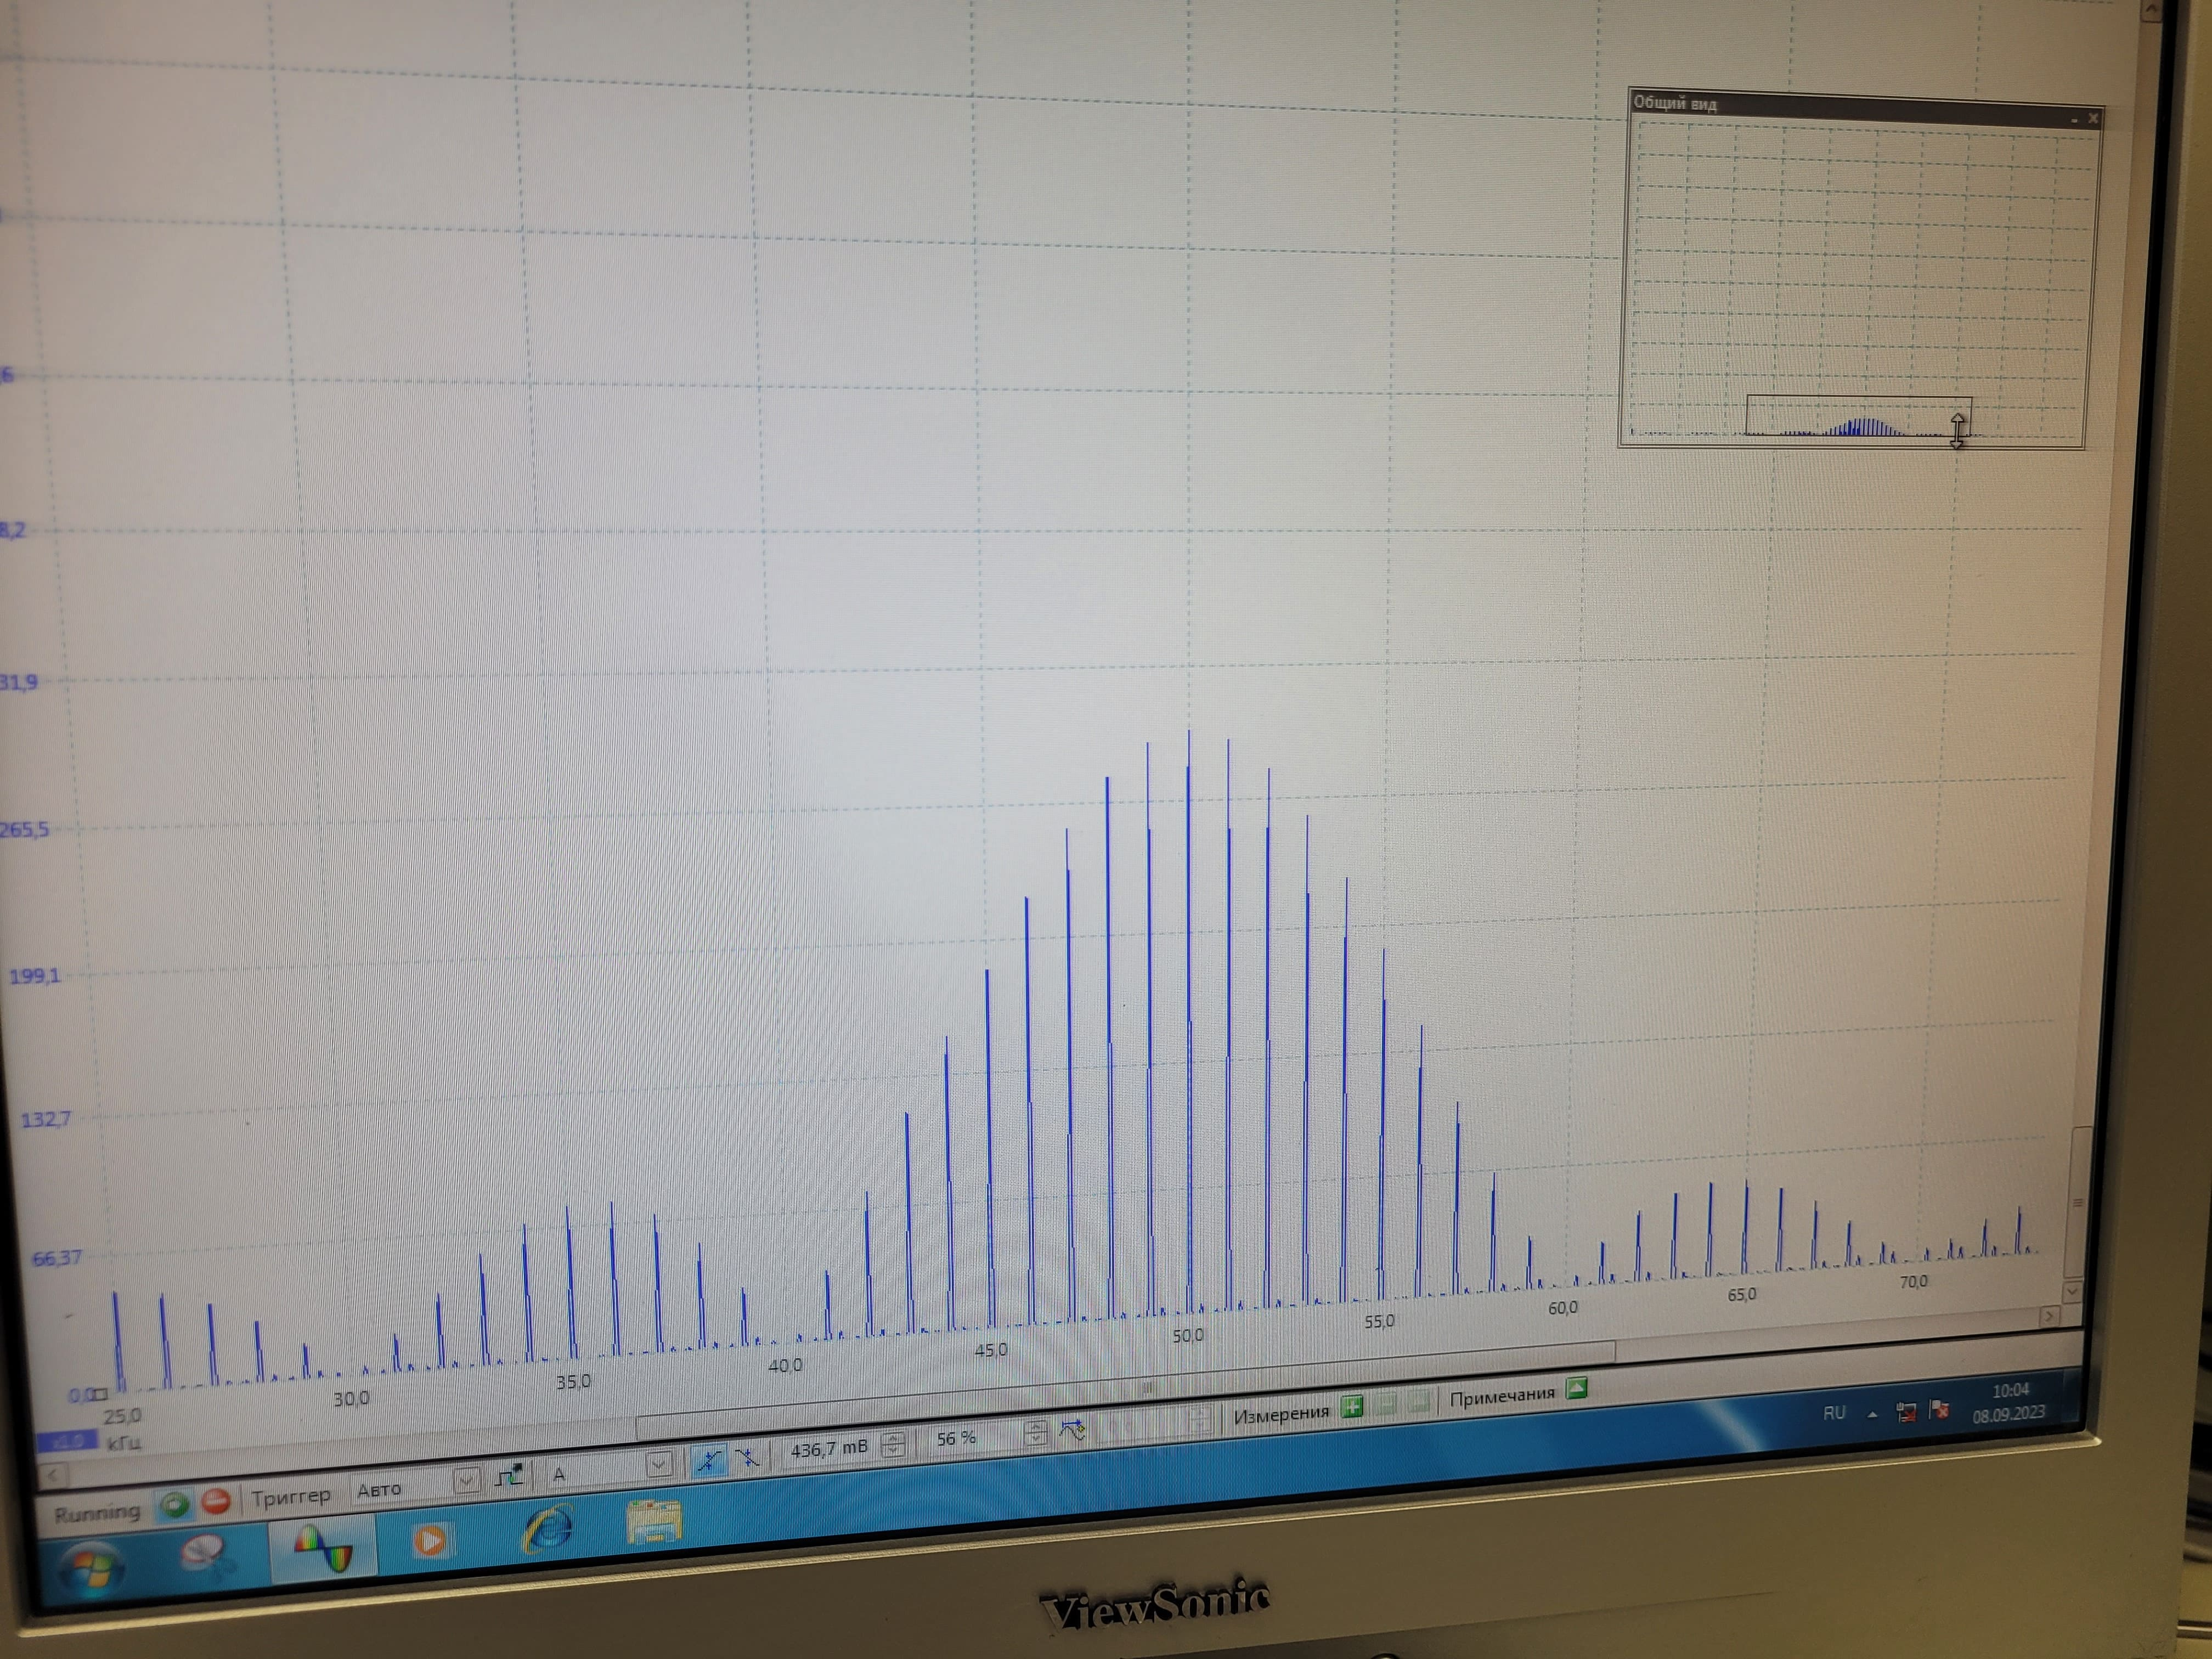
\includegraphics[width=1\linewidth]{B_50k_1k_5.jpg}} $\nu_\text{повт}$  = 1 кГц, $\delta \nu$ = 1 кГц, $\Delta \nu$ = 10 кГц \\
\end{minipage}
\hfill
\begin{minipage}[h]{0.47\linewidth}
\center{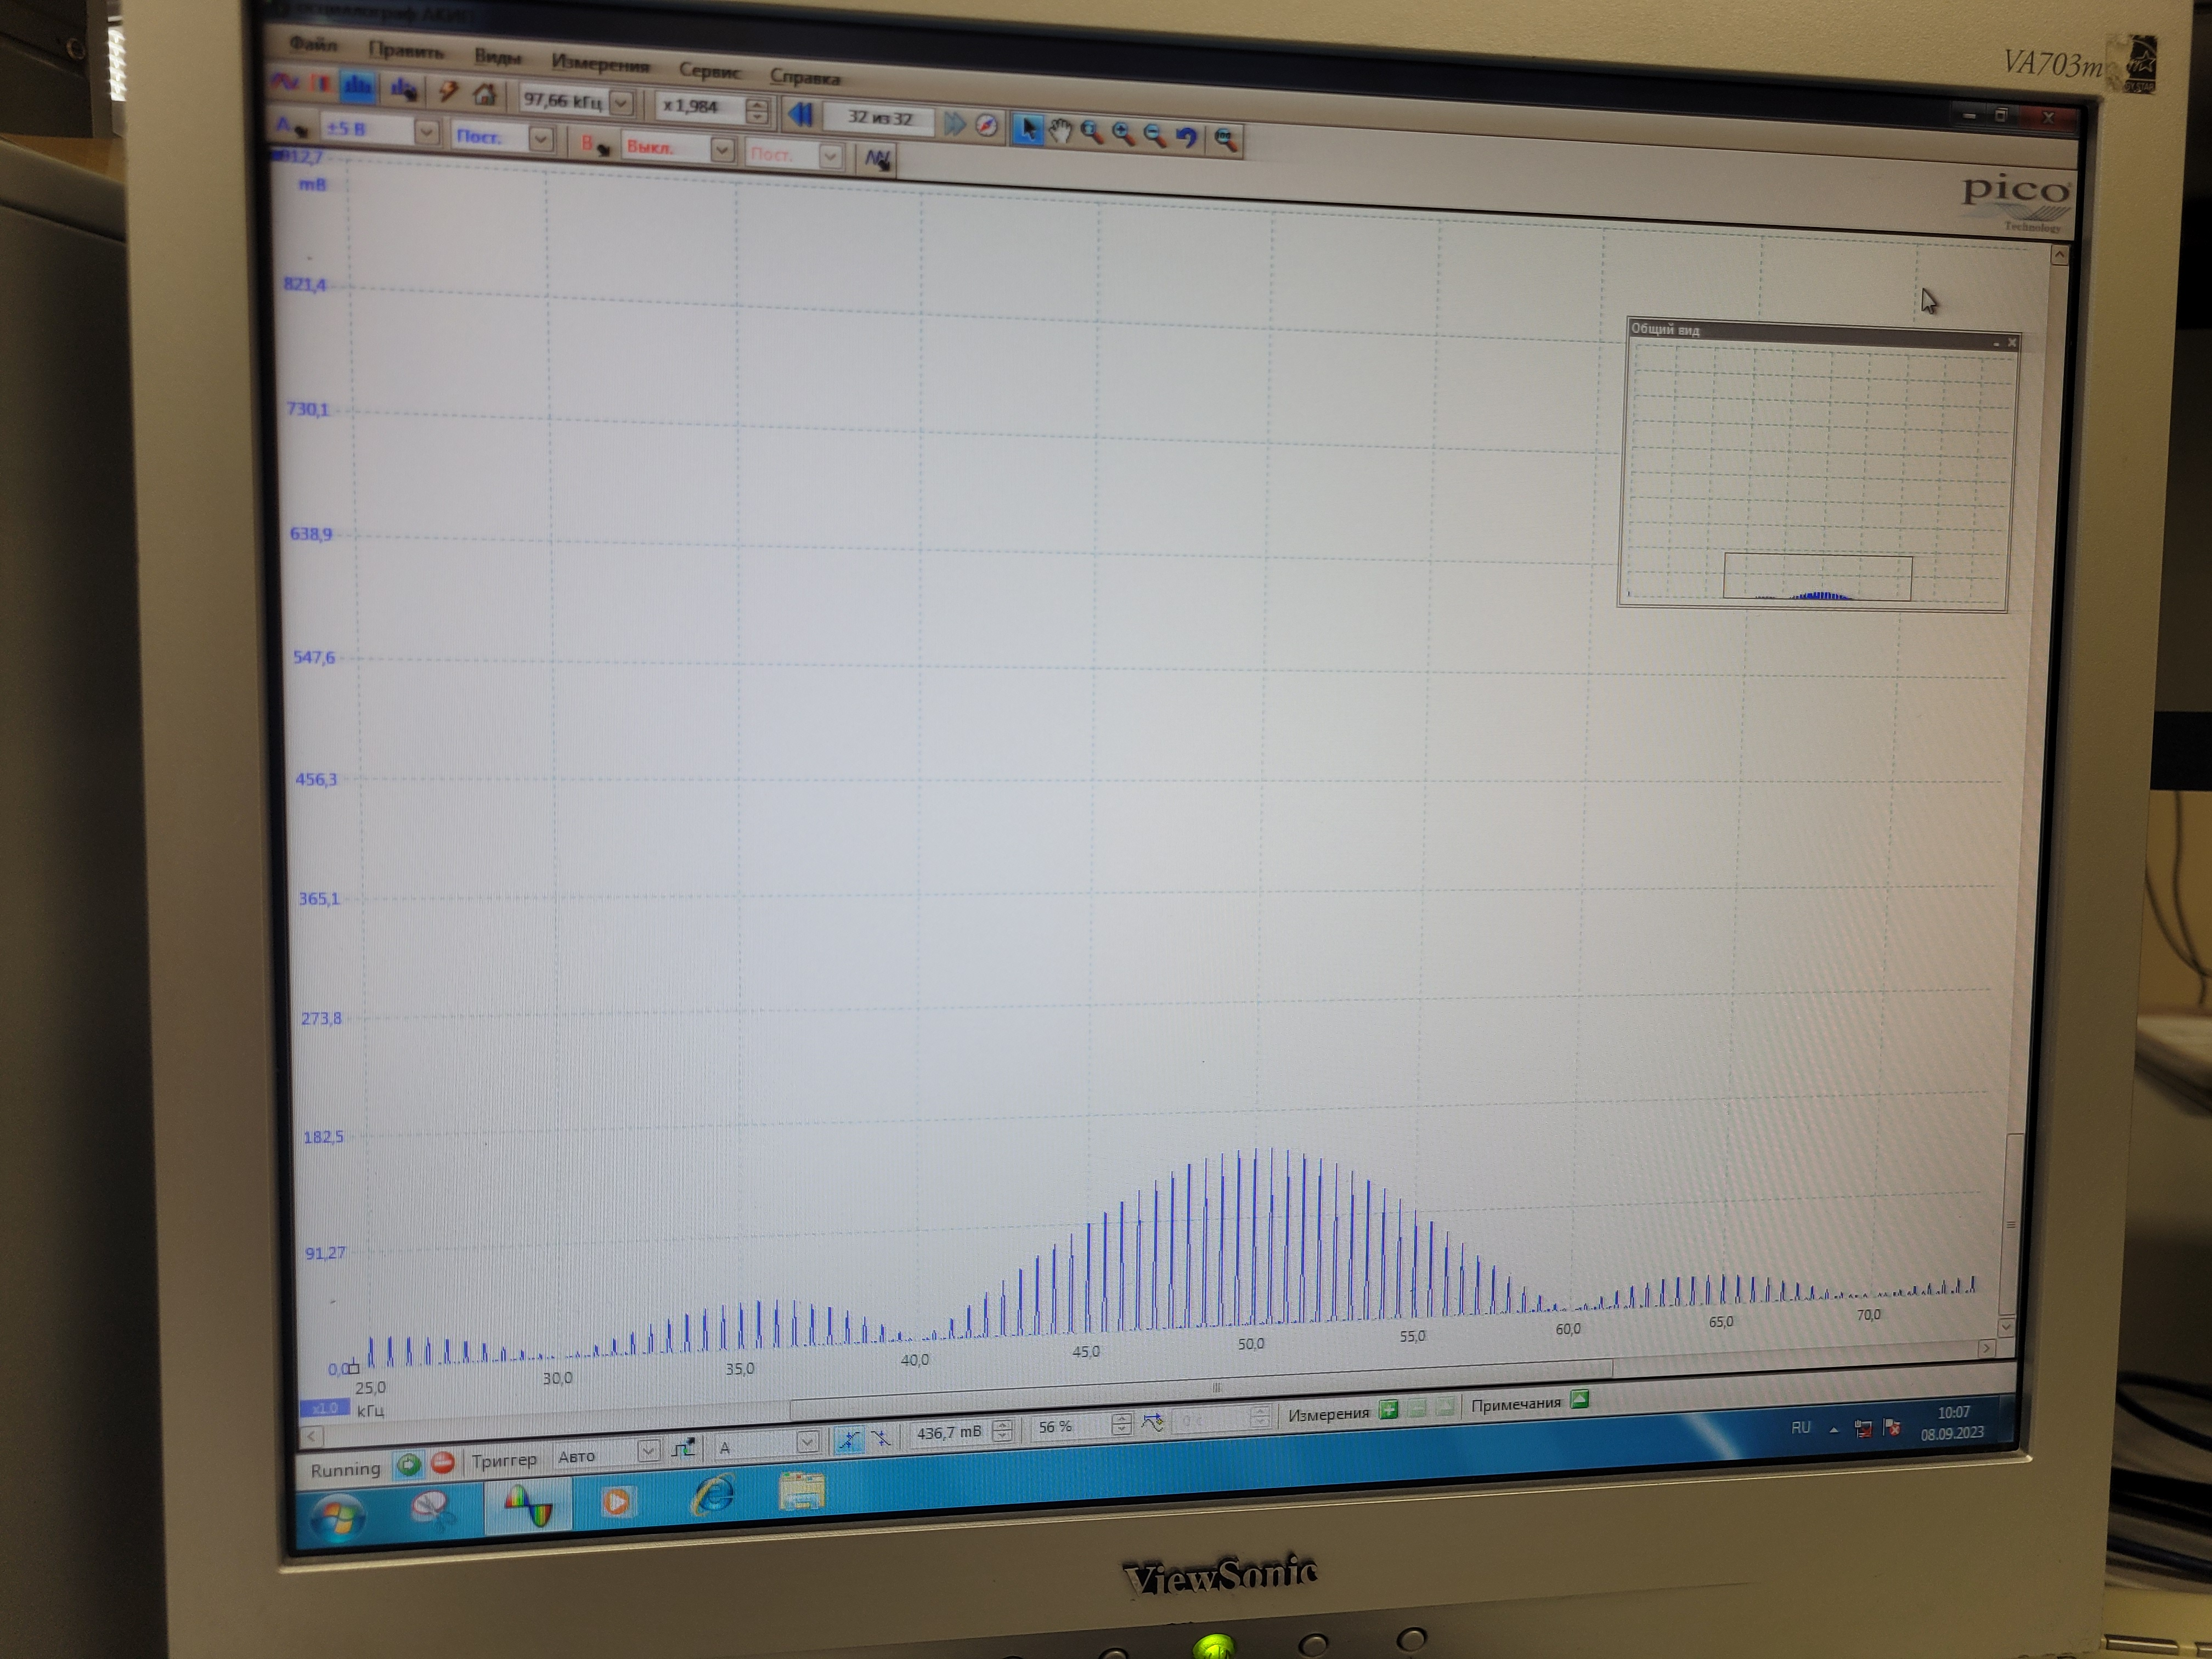
\includegraphics[width=1\linewidth]{B_50k_2k_5.jpg}} \\ $\nu_\text{повт}$  = 0.5 кГц, $\delta \nu$ = 0.5 кГц, $\Delta \nu$ = 10 кГц
\end{minipage}
\vfill
\begin{minipage}[h]{0.47\linewidth}
\center{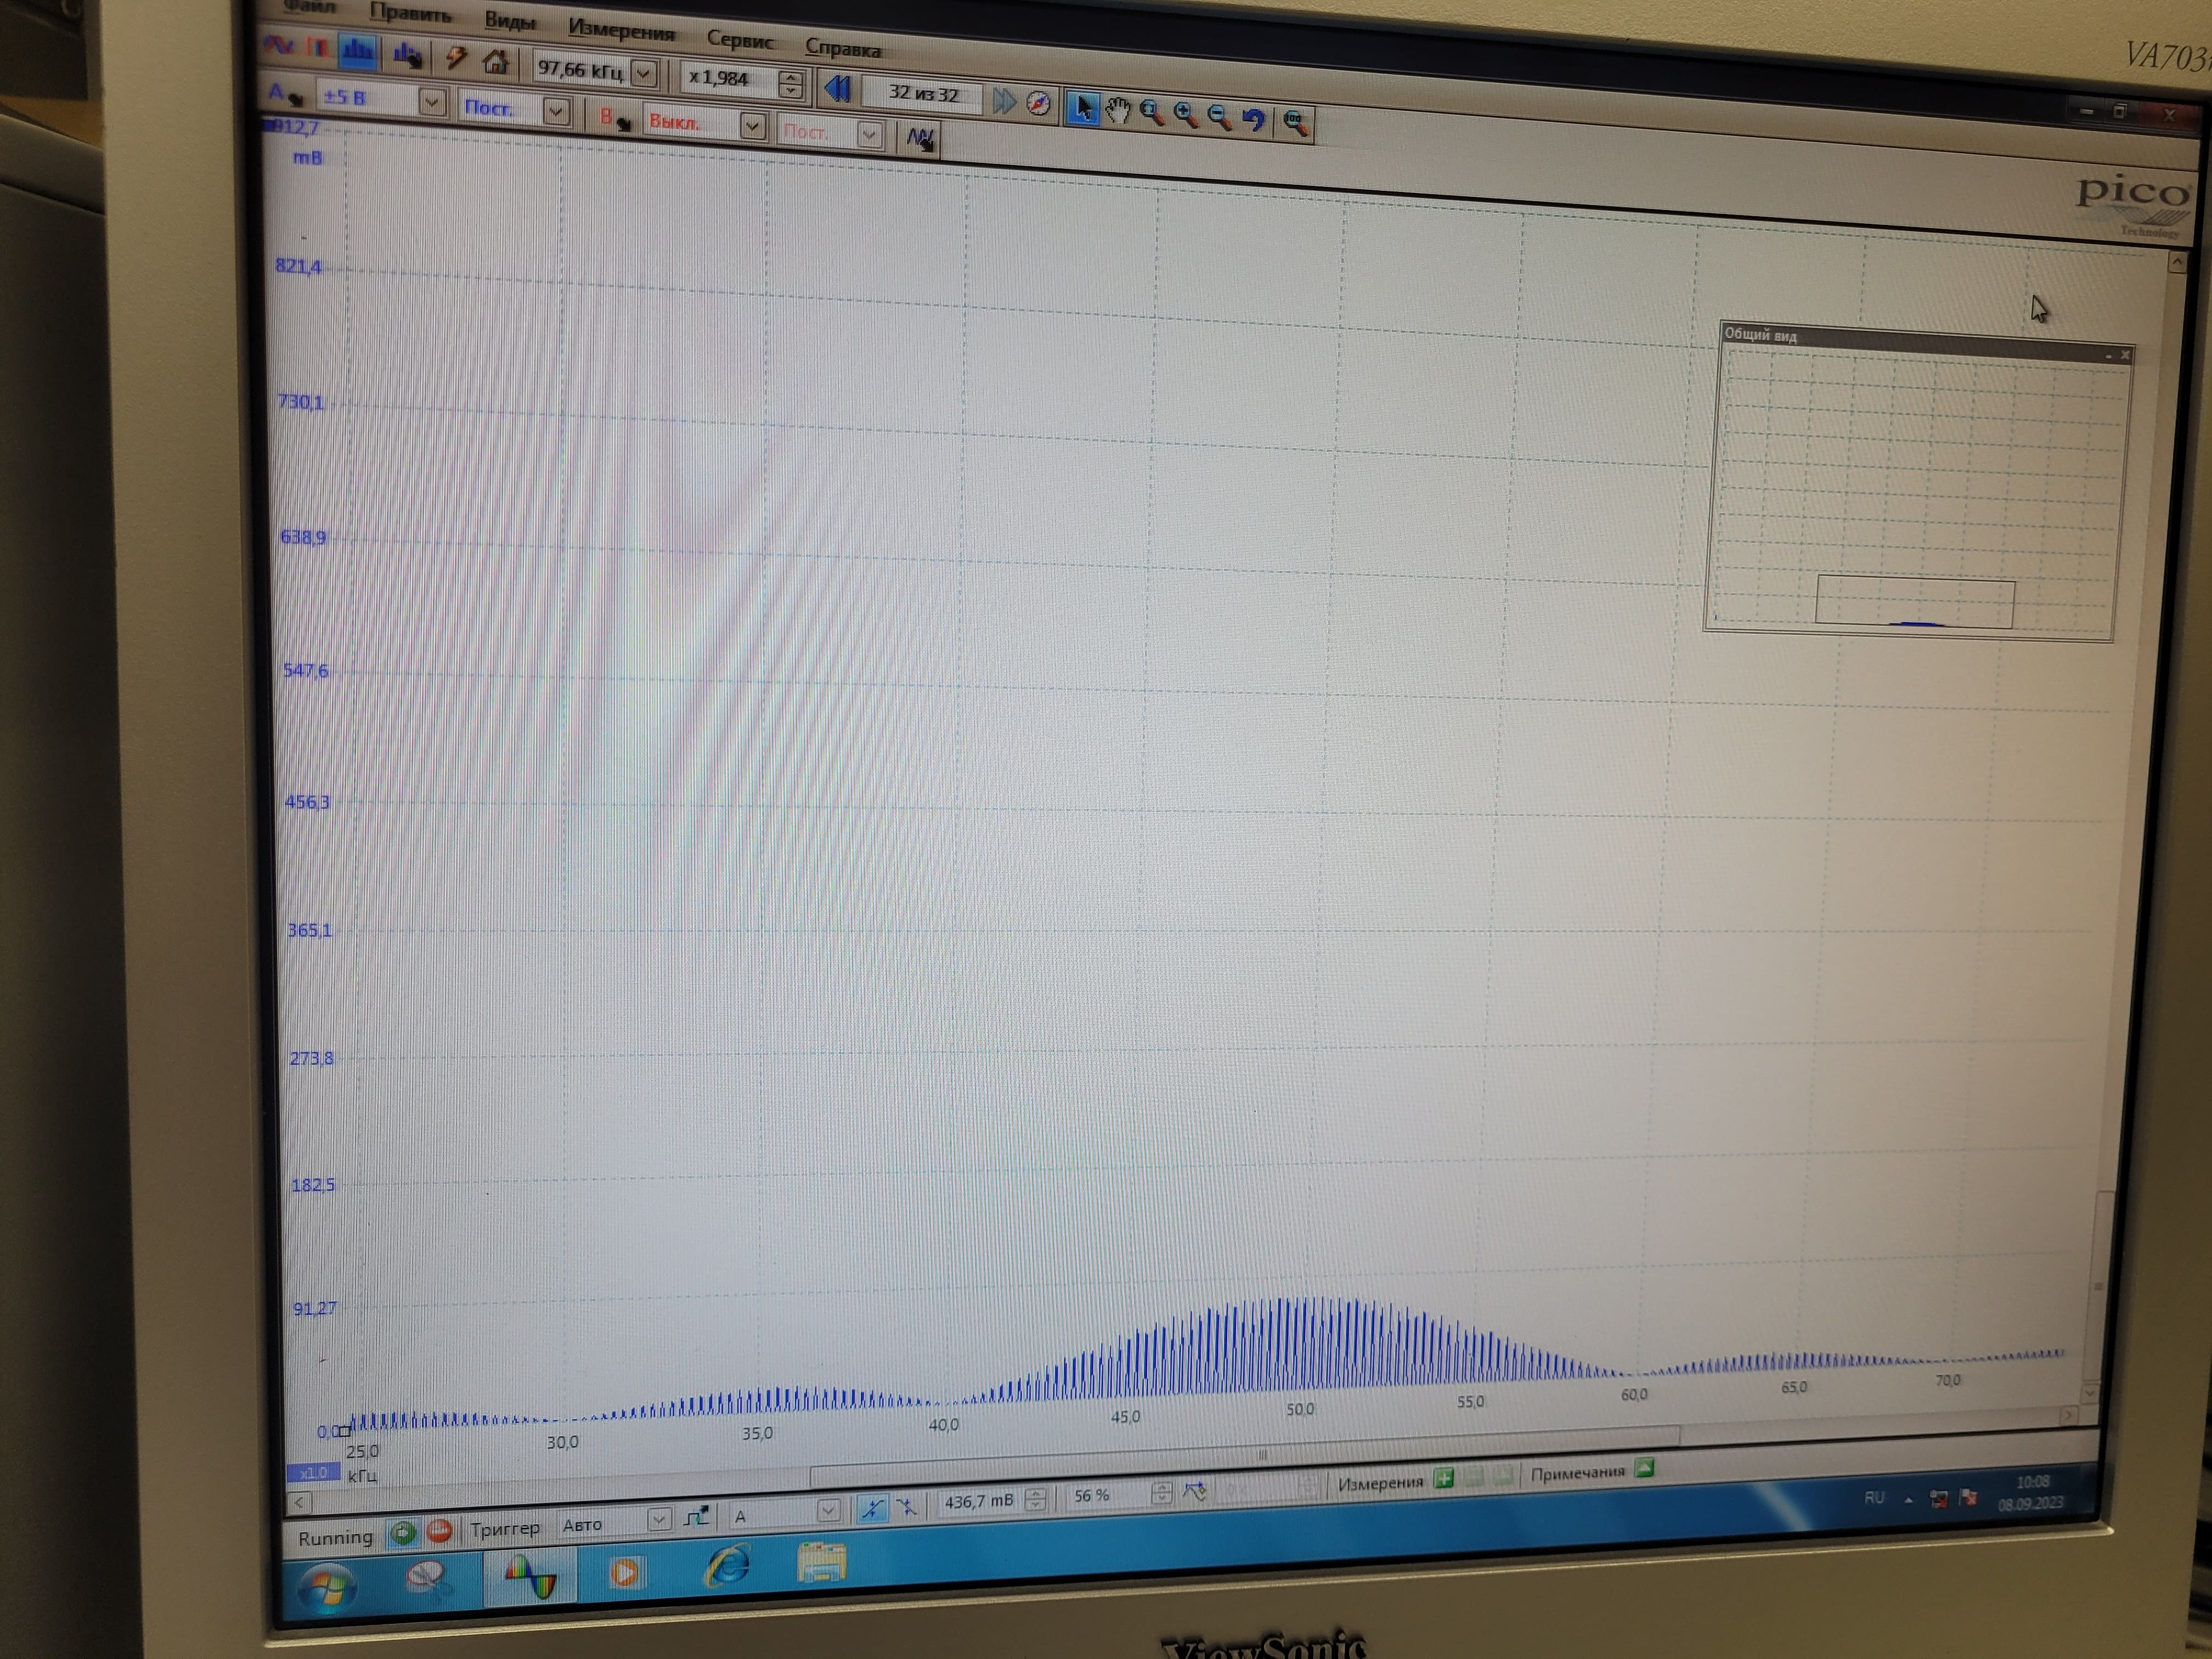
\includegraphics[width=1\linewidth]{B_50k_4k_5.jpg}} $\nu_\text{повт}$  = 0.25 кГц, $\delta \nu$ = 0.25 кГц, $\Delta \nu$ = 10 кГц \\
\end{minipage}
\hfill
\caption{}
\label{ris:experimentalcorrelationsignals}
\end{figure}

Видно, что соотношение неопределённости выполняется:
$$ \frac{\delta \nu}{\nu_\text{повт}} = \frac{1\cdot10^3}{1\cdot10^3} = \frac{0.5\cdot10^3}{0.5\cdot10^3} = \frac{0.25\cdot10^3}{0.25\cdot10^3} = 1 $$\\

Также видно, что при стремлении частоты повторения к нулю, стремится к нулю и расстояние между компонентами спектра.

\end{enumerate}


















\newpage

\subsection*{В. Наблюдение спектра периодической последовательности гауссианов}
\begin{figure}[h]
    \centering
    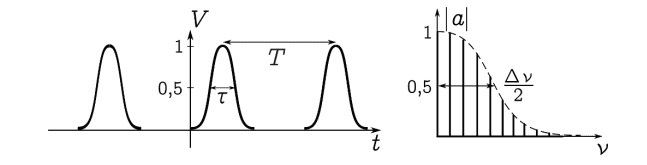
\includegraphics[width=0.7\linewidth]{gausiana.png}
    \caption{Периодическая последовательность гауссианов и ее спектр}
    \label{gausiana}
\end{figure}

\begin{enumerate}


\item [\textbf{1.}] Настраиваем генератор в режим передачи периодической последовательности \textit{"гауссианов"} с несущей частотой $\nu_0$ = 50 кГц и периодом повторения $T$ = 10 мс.

\item [\textbf{2.}] Получаем на экране спектр (Преобразование Фурье) сигнала.

\textbf{a.} Изменяем $\nu_0$ при фиксированных $T$ = 10 мс.


\begin{figure}[h]
\begin{minipage}[h]{0.47\linewidth}
\center{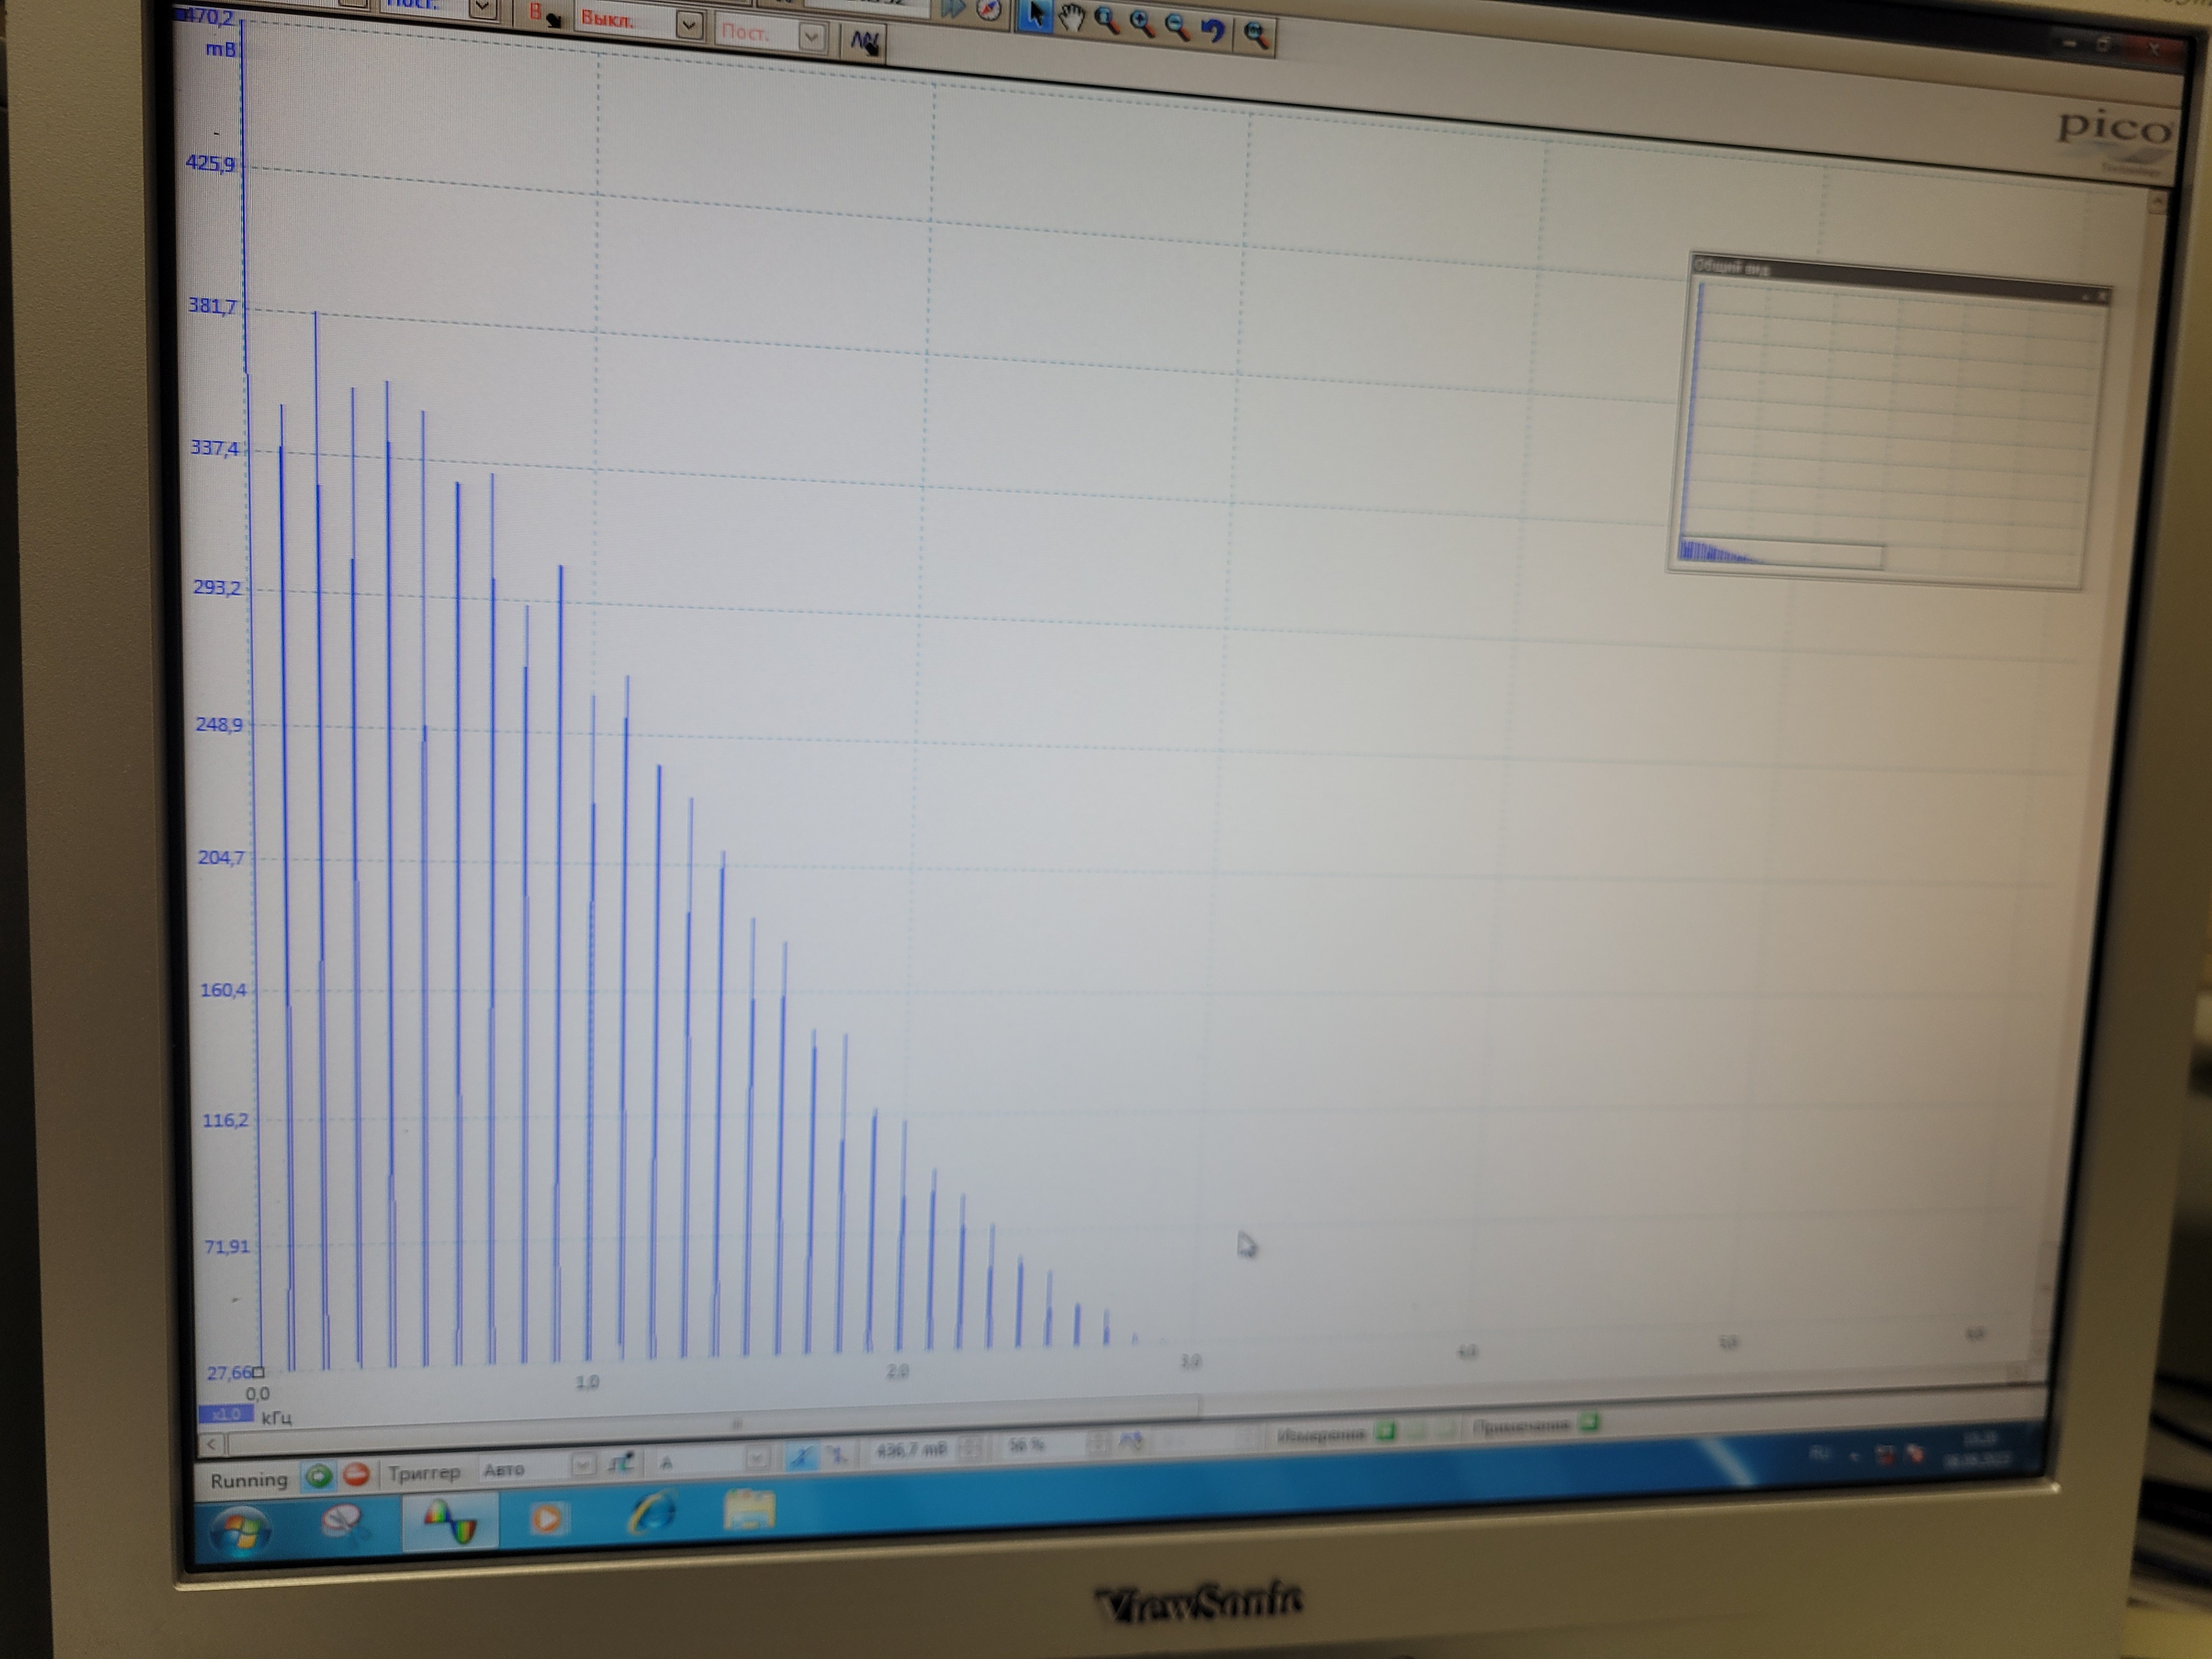
\includegraphics[width=1\linewidth]{V_1k_10T.jpg}} $\nu$ = 1 кГц \\
\end{minipage}
\hfill
\begin{minipage}[h]{0.47\linewidth}
\center{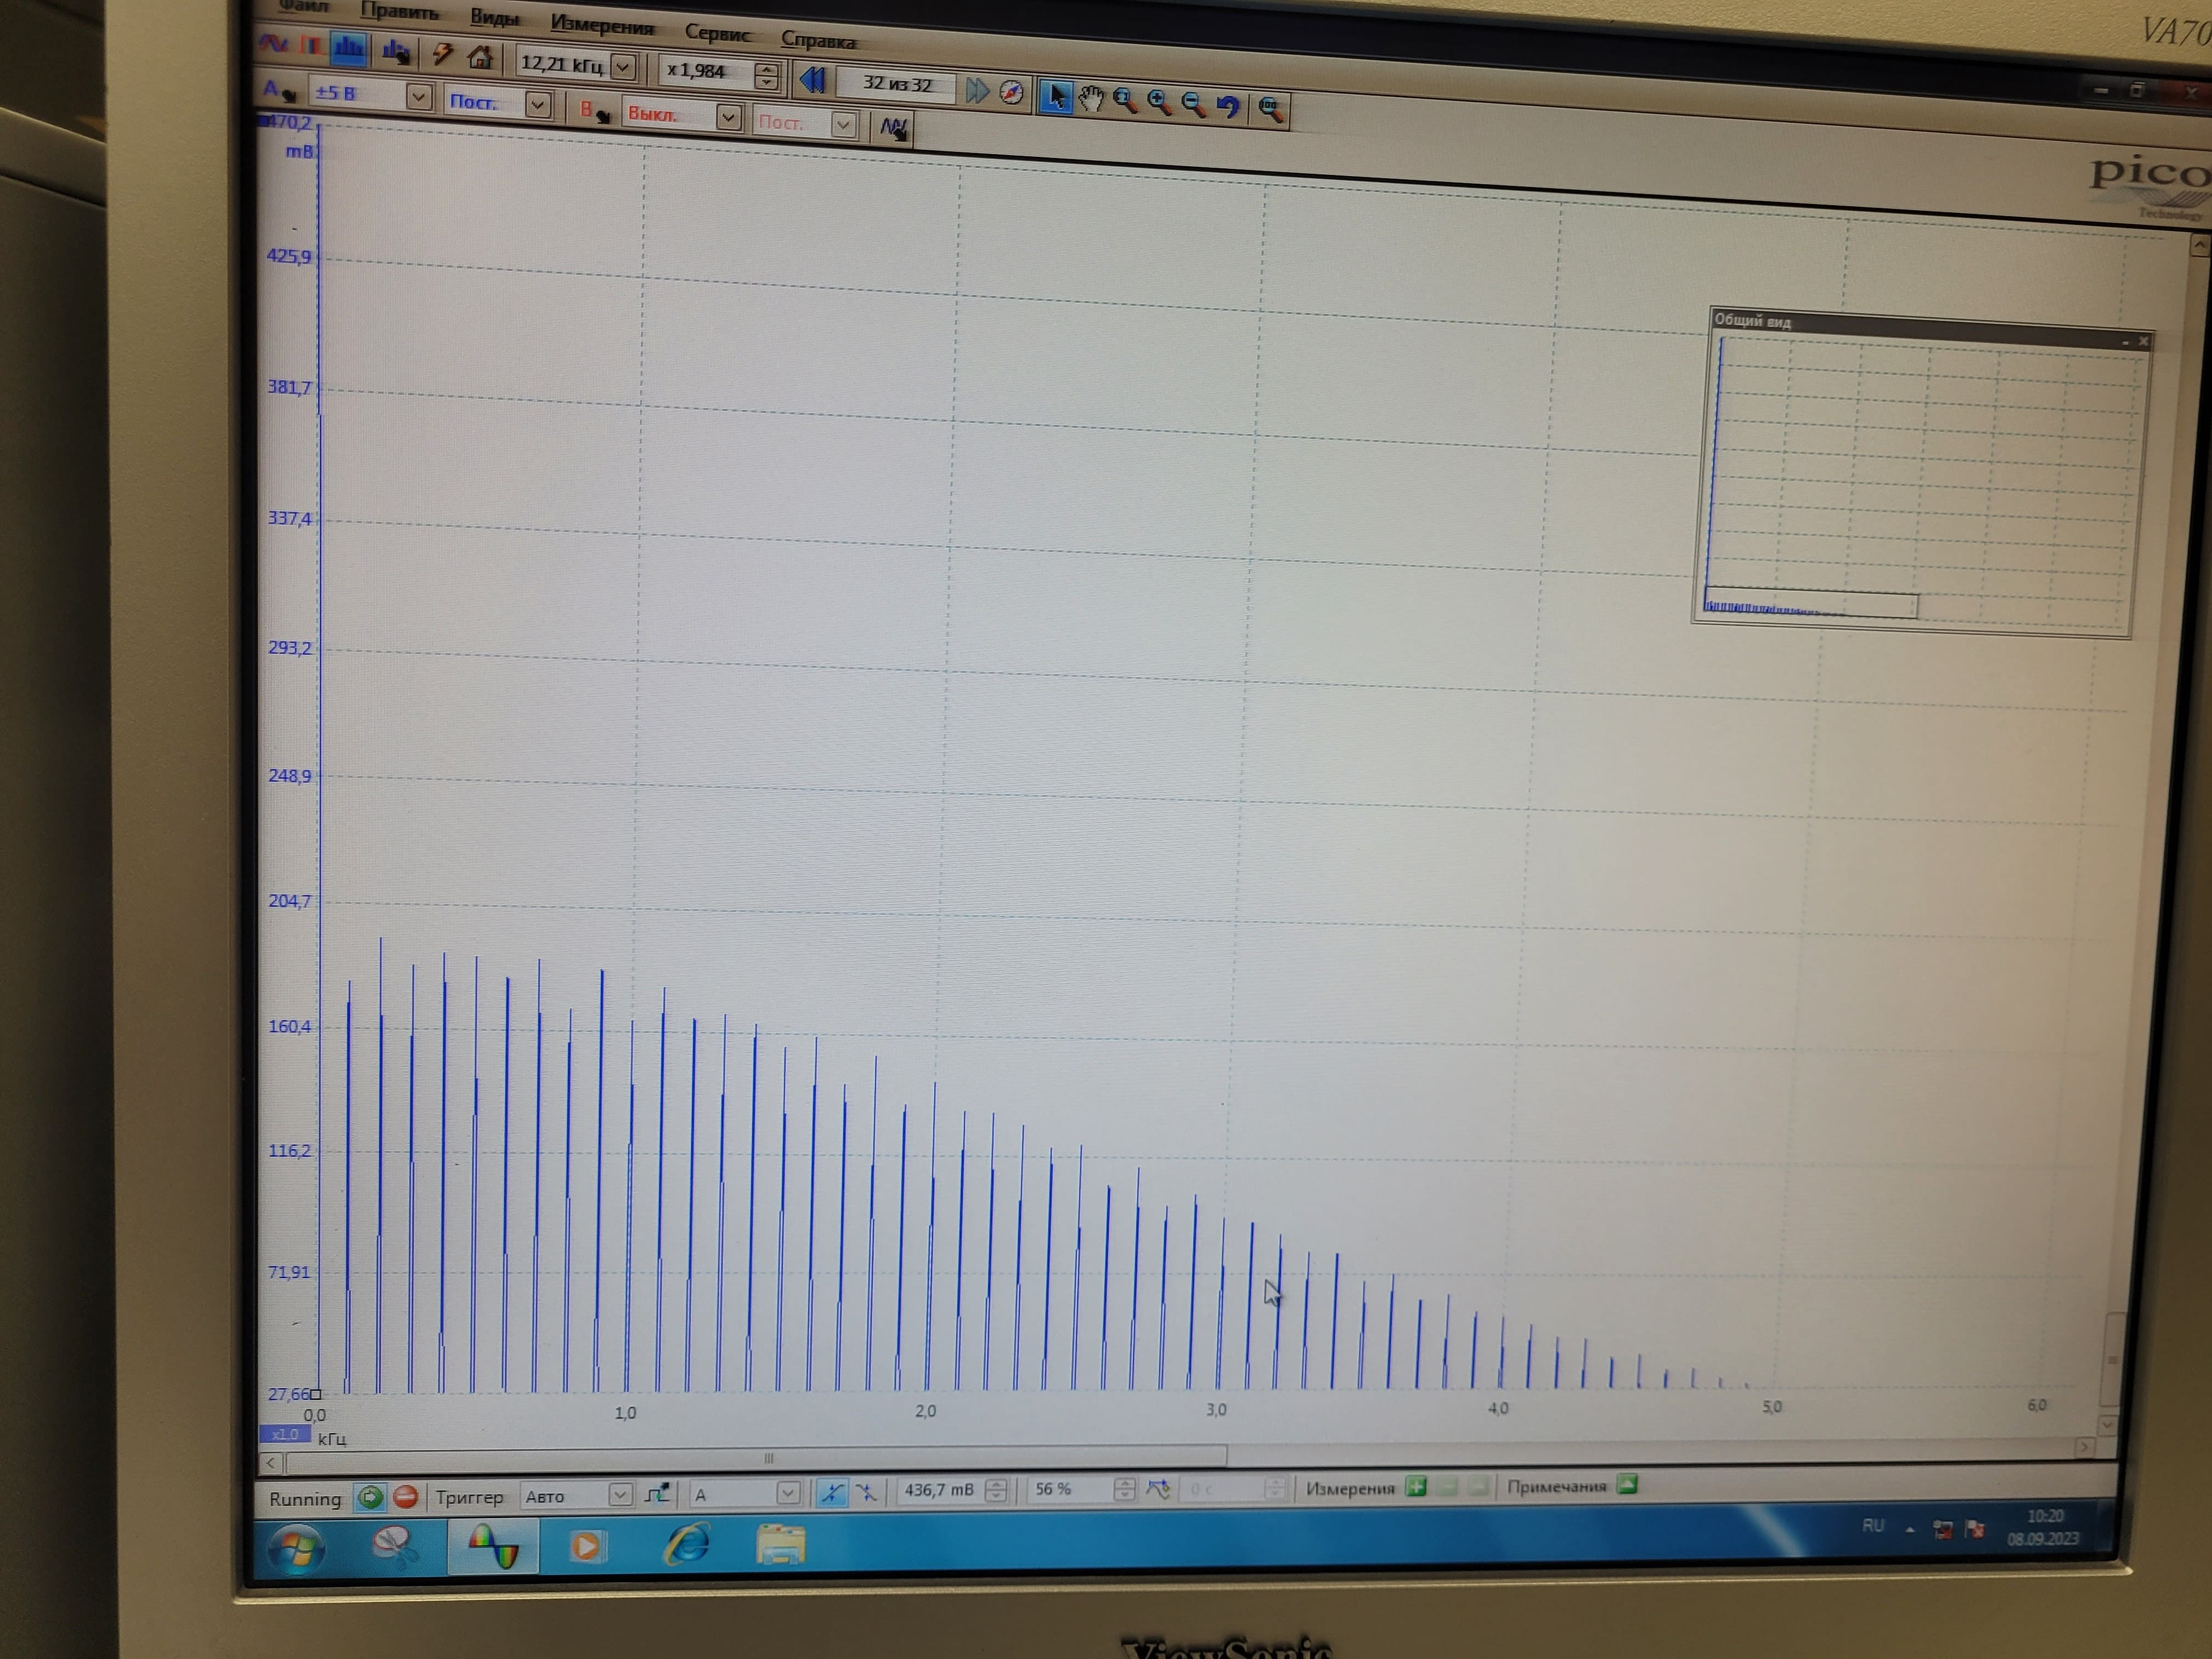
\includegraphics[width=1\linewidth]{V_2k_10T.jpg}} \\$\nu$ = 2 кГц 
\end{minipage}
\vfill
\begin{minipage}[h]{0.47\linewidth}
\center{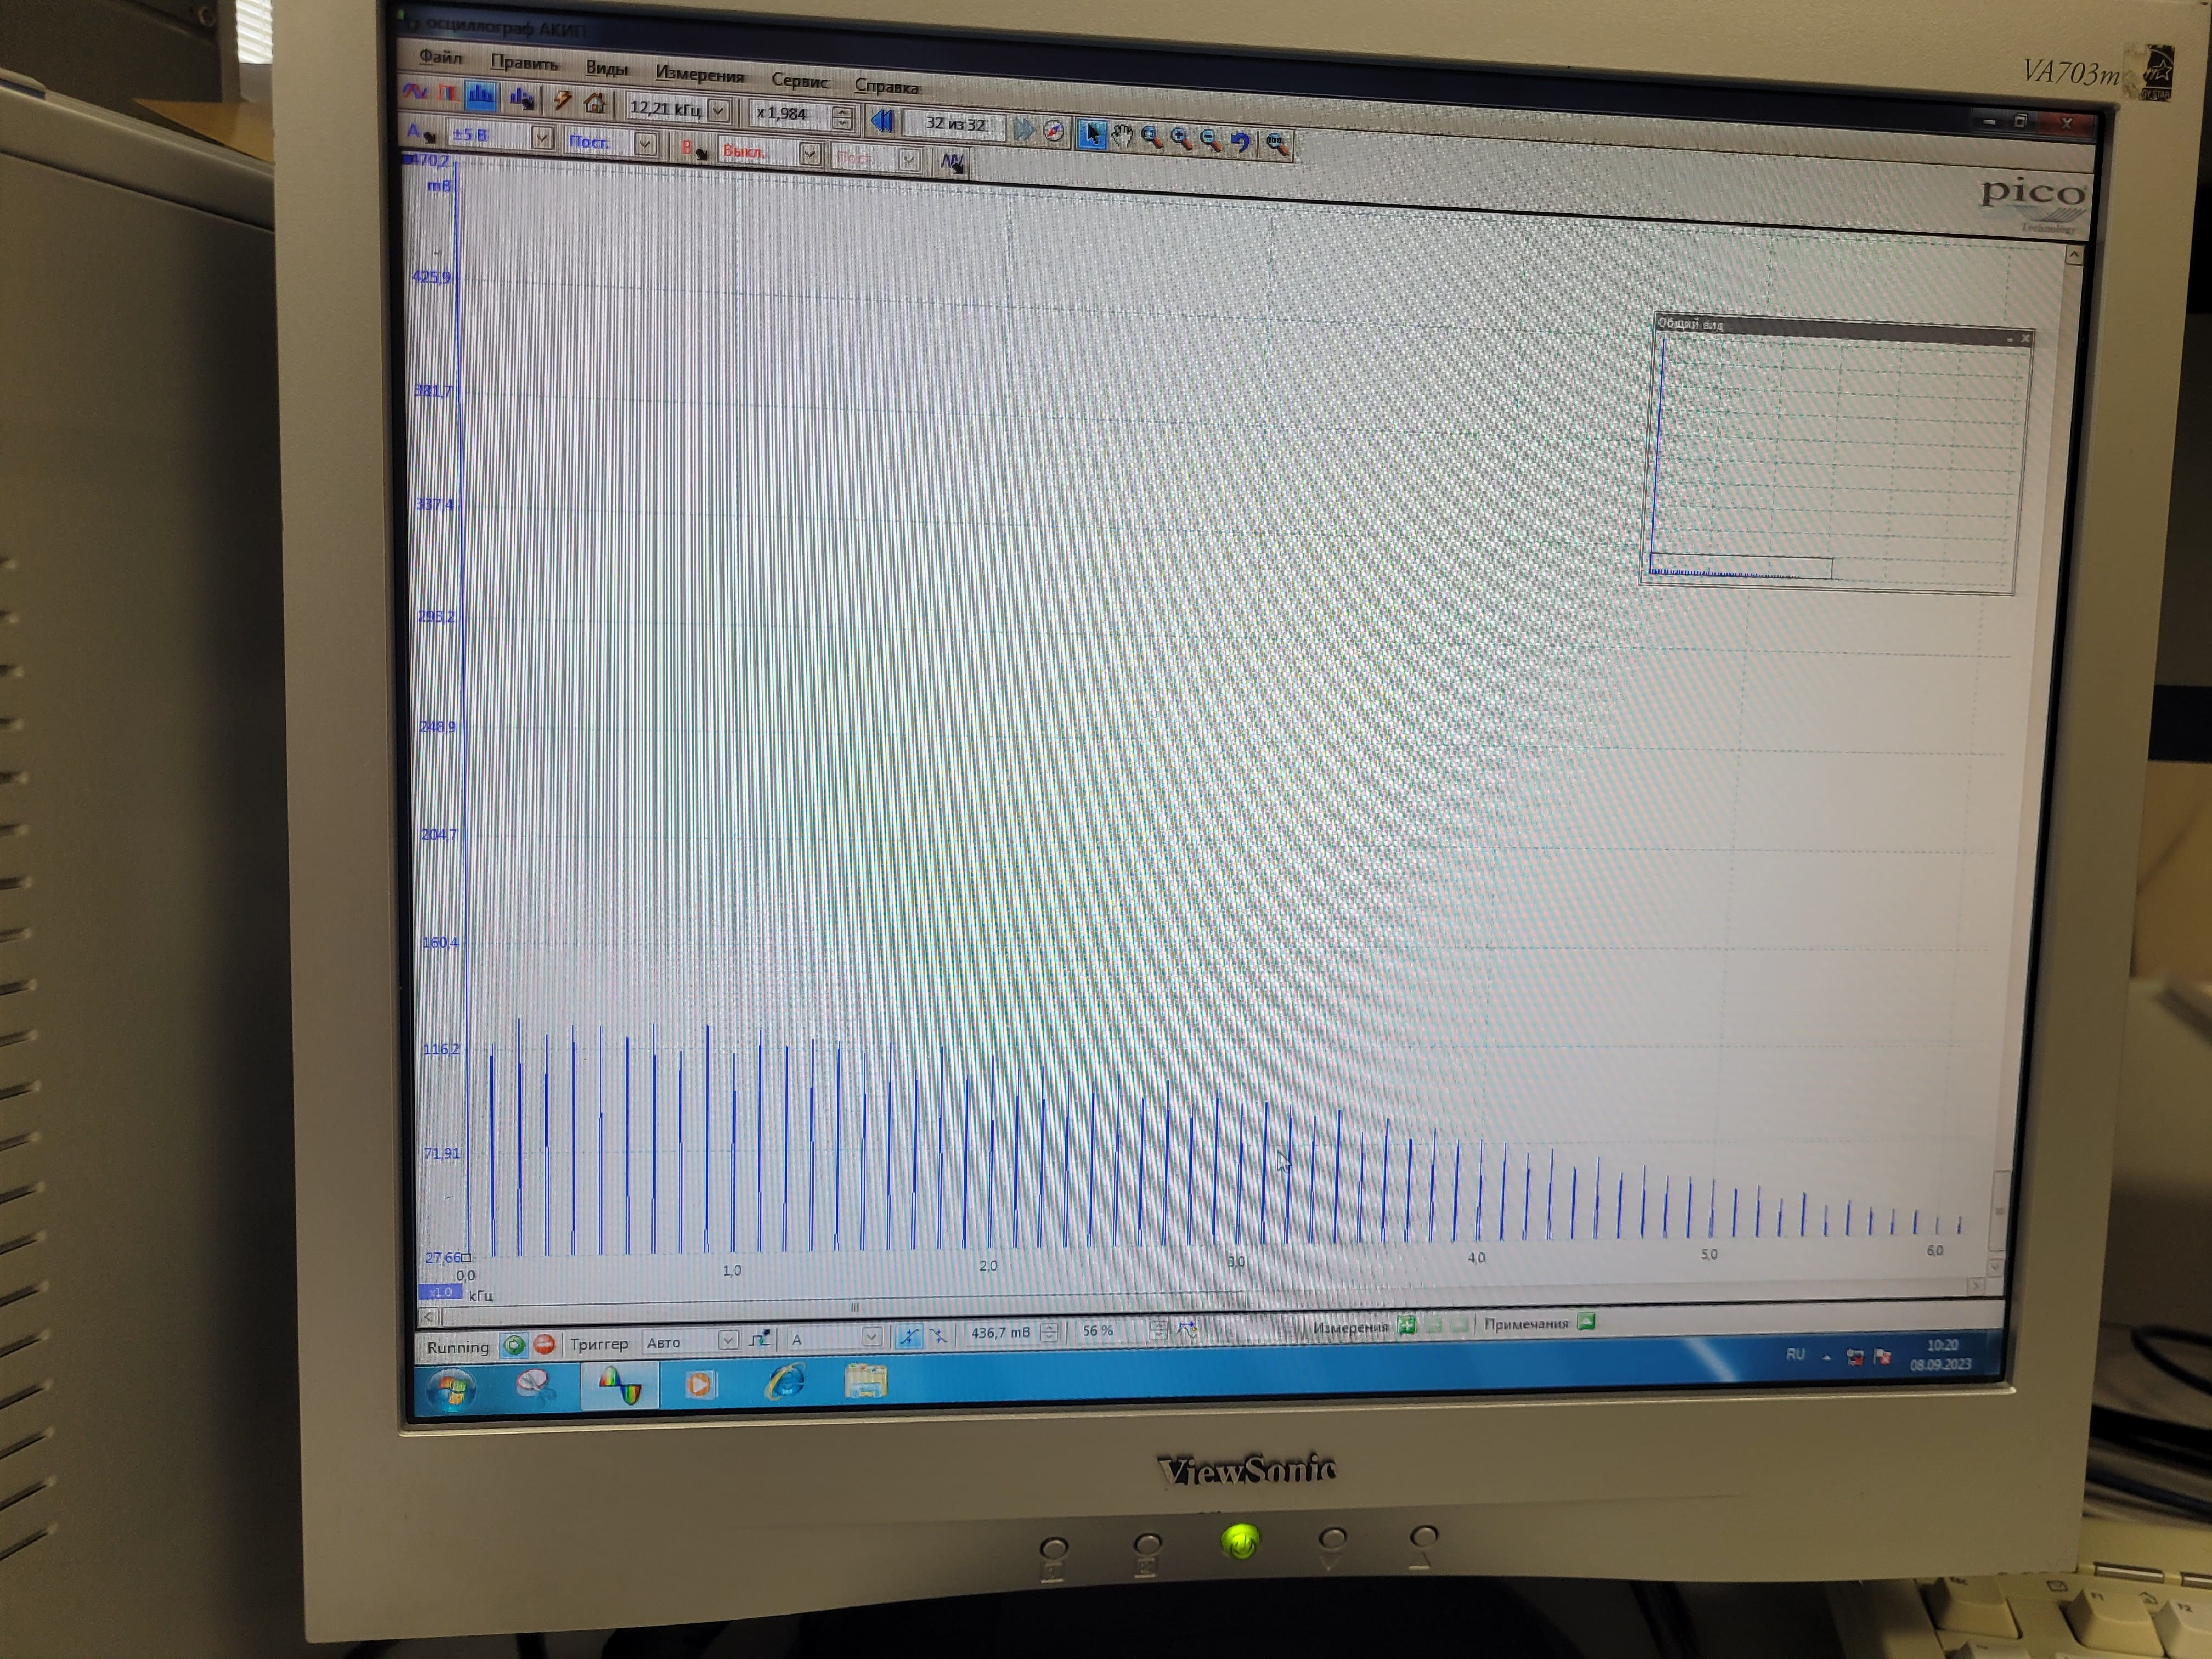
\includegraphics[width=1\linewidth]{V_3k_10T.jpg}} $\nu$ = 1 3Гц \\
\end{minipage}
\hfill
\caption{}
\label{ris:experimentalcorrelationsignals}
\end{figure}


\newpage

\textbf{б.} Изменяем $T$ при фиксированных $\nu_0$ = 1 кГц.


\begin{figure}[h]
\begin{minipage}[h]{0.47\linewidth}
\center{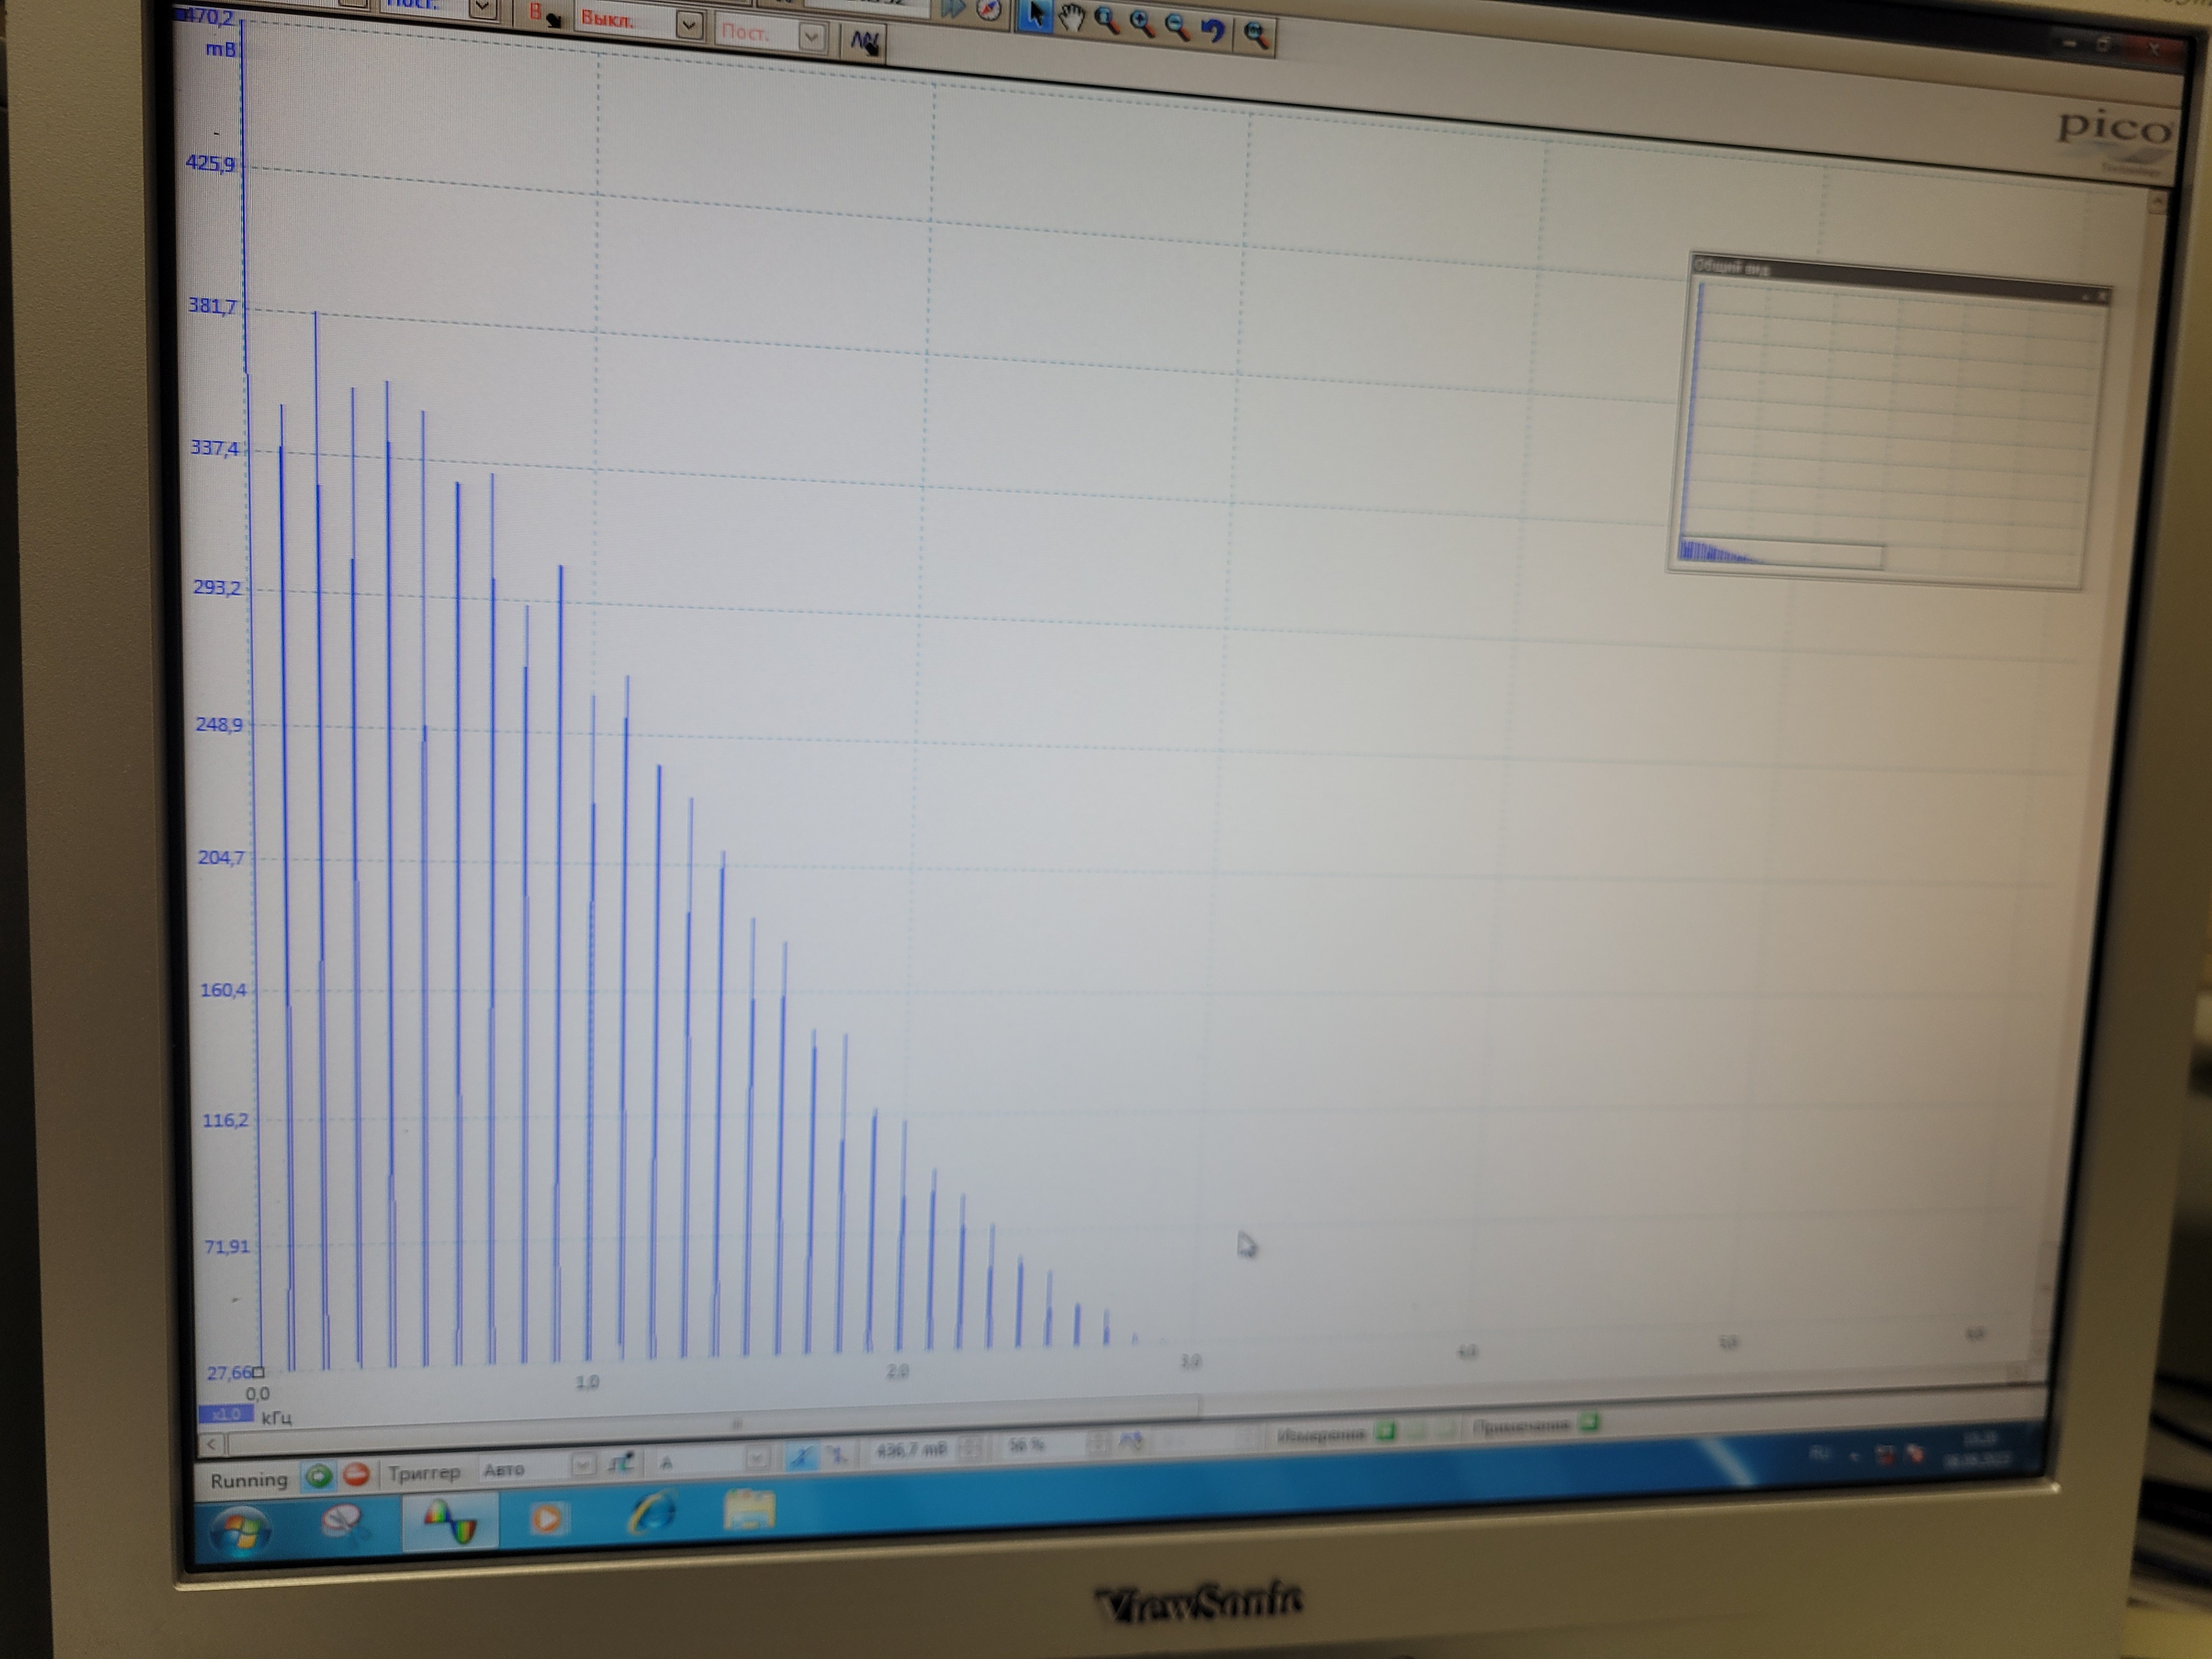
\includegraphics[width=1\linewidth]{V_1k_10T.jpg}} $T$ = 10 мс \\
\end{minipage}
\hfill
\begin{minipage}[h]{0.47\linewidth}
\center{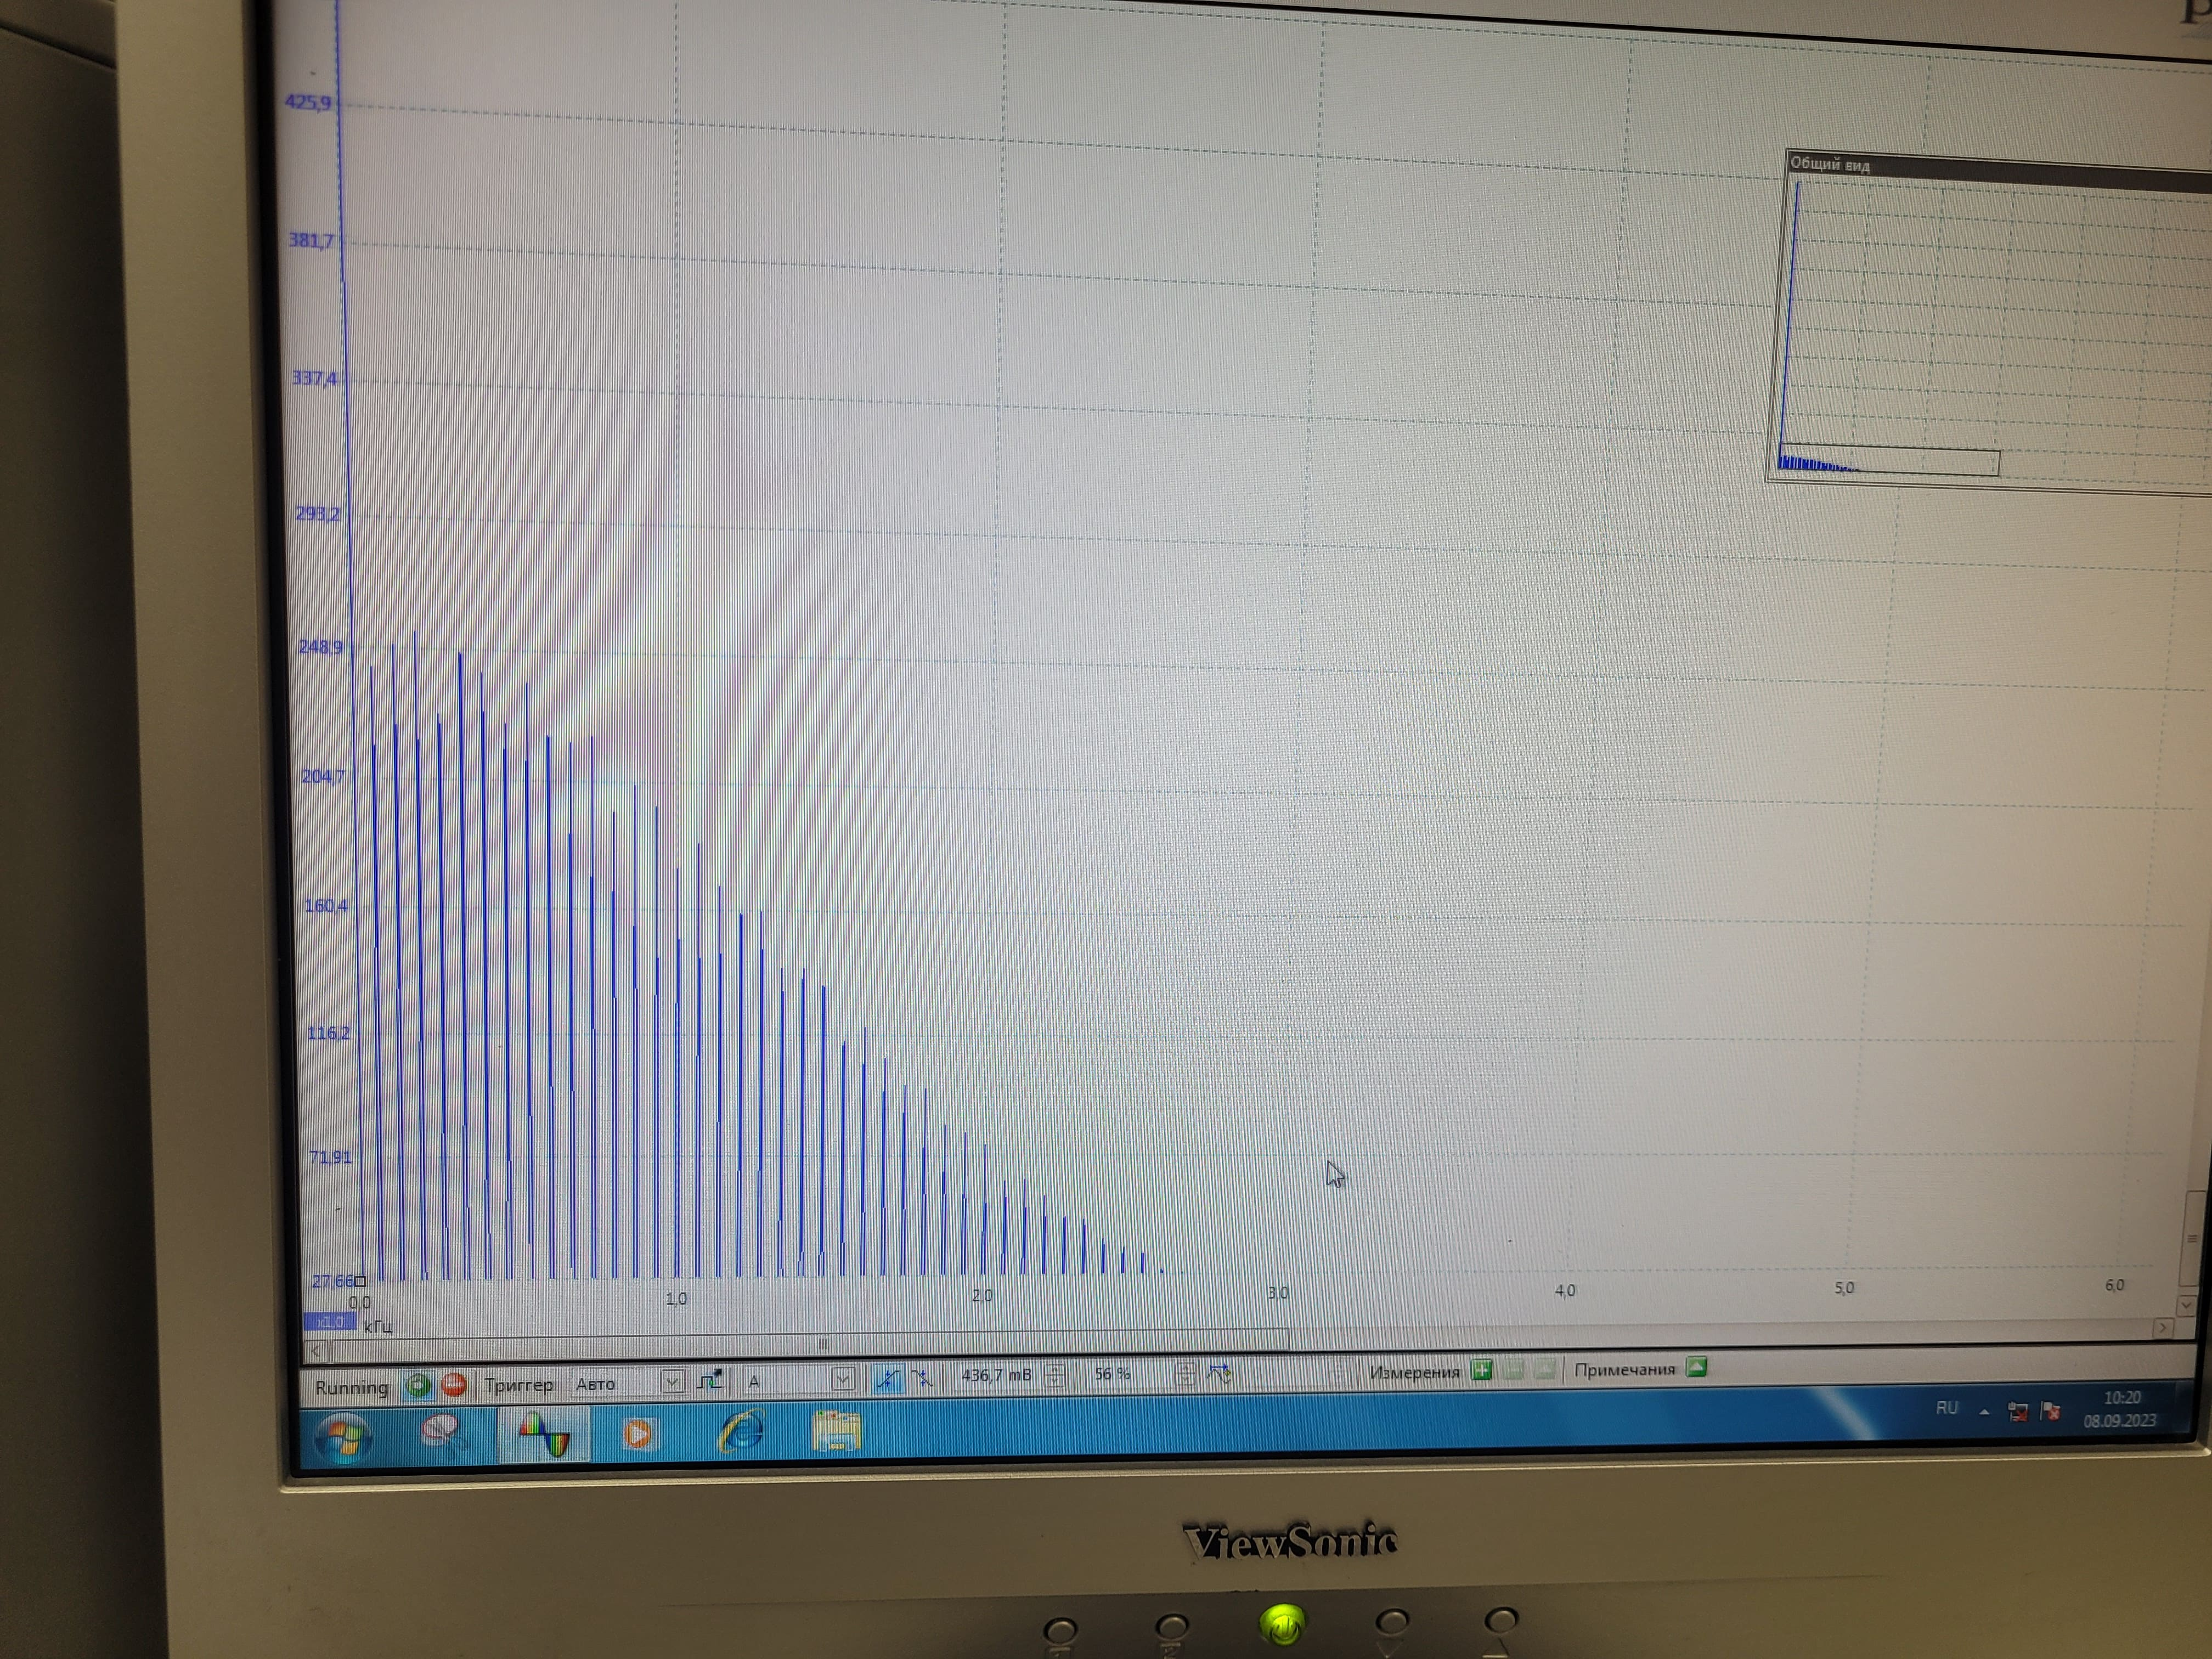
\includegraphics[width=1\linewidth]{V_1k_15T.jpg}} \\  $T$ = 15 мс 
\end{minipage}
\vfill
\begin{minipage}[h]{0.47\linewidth}
\center{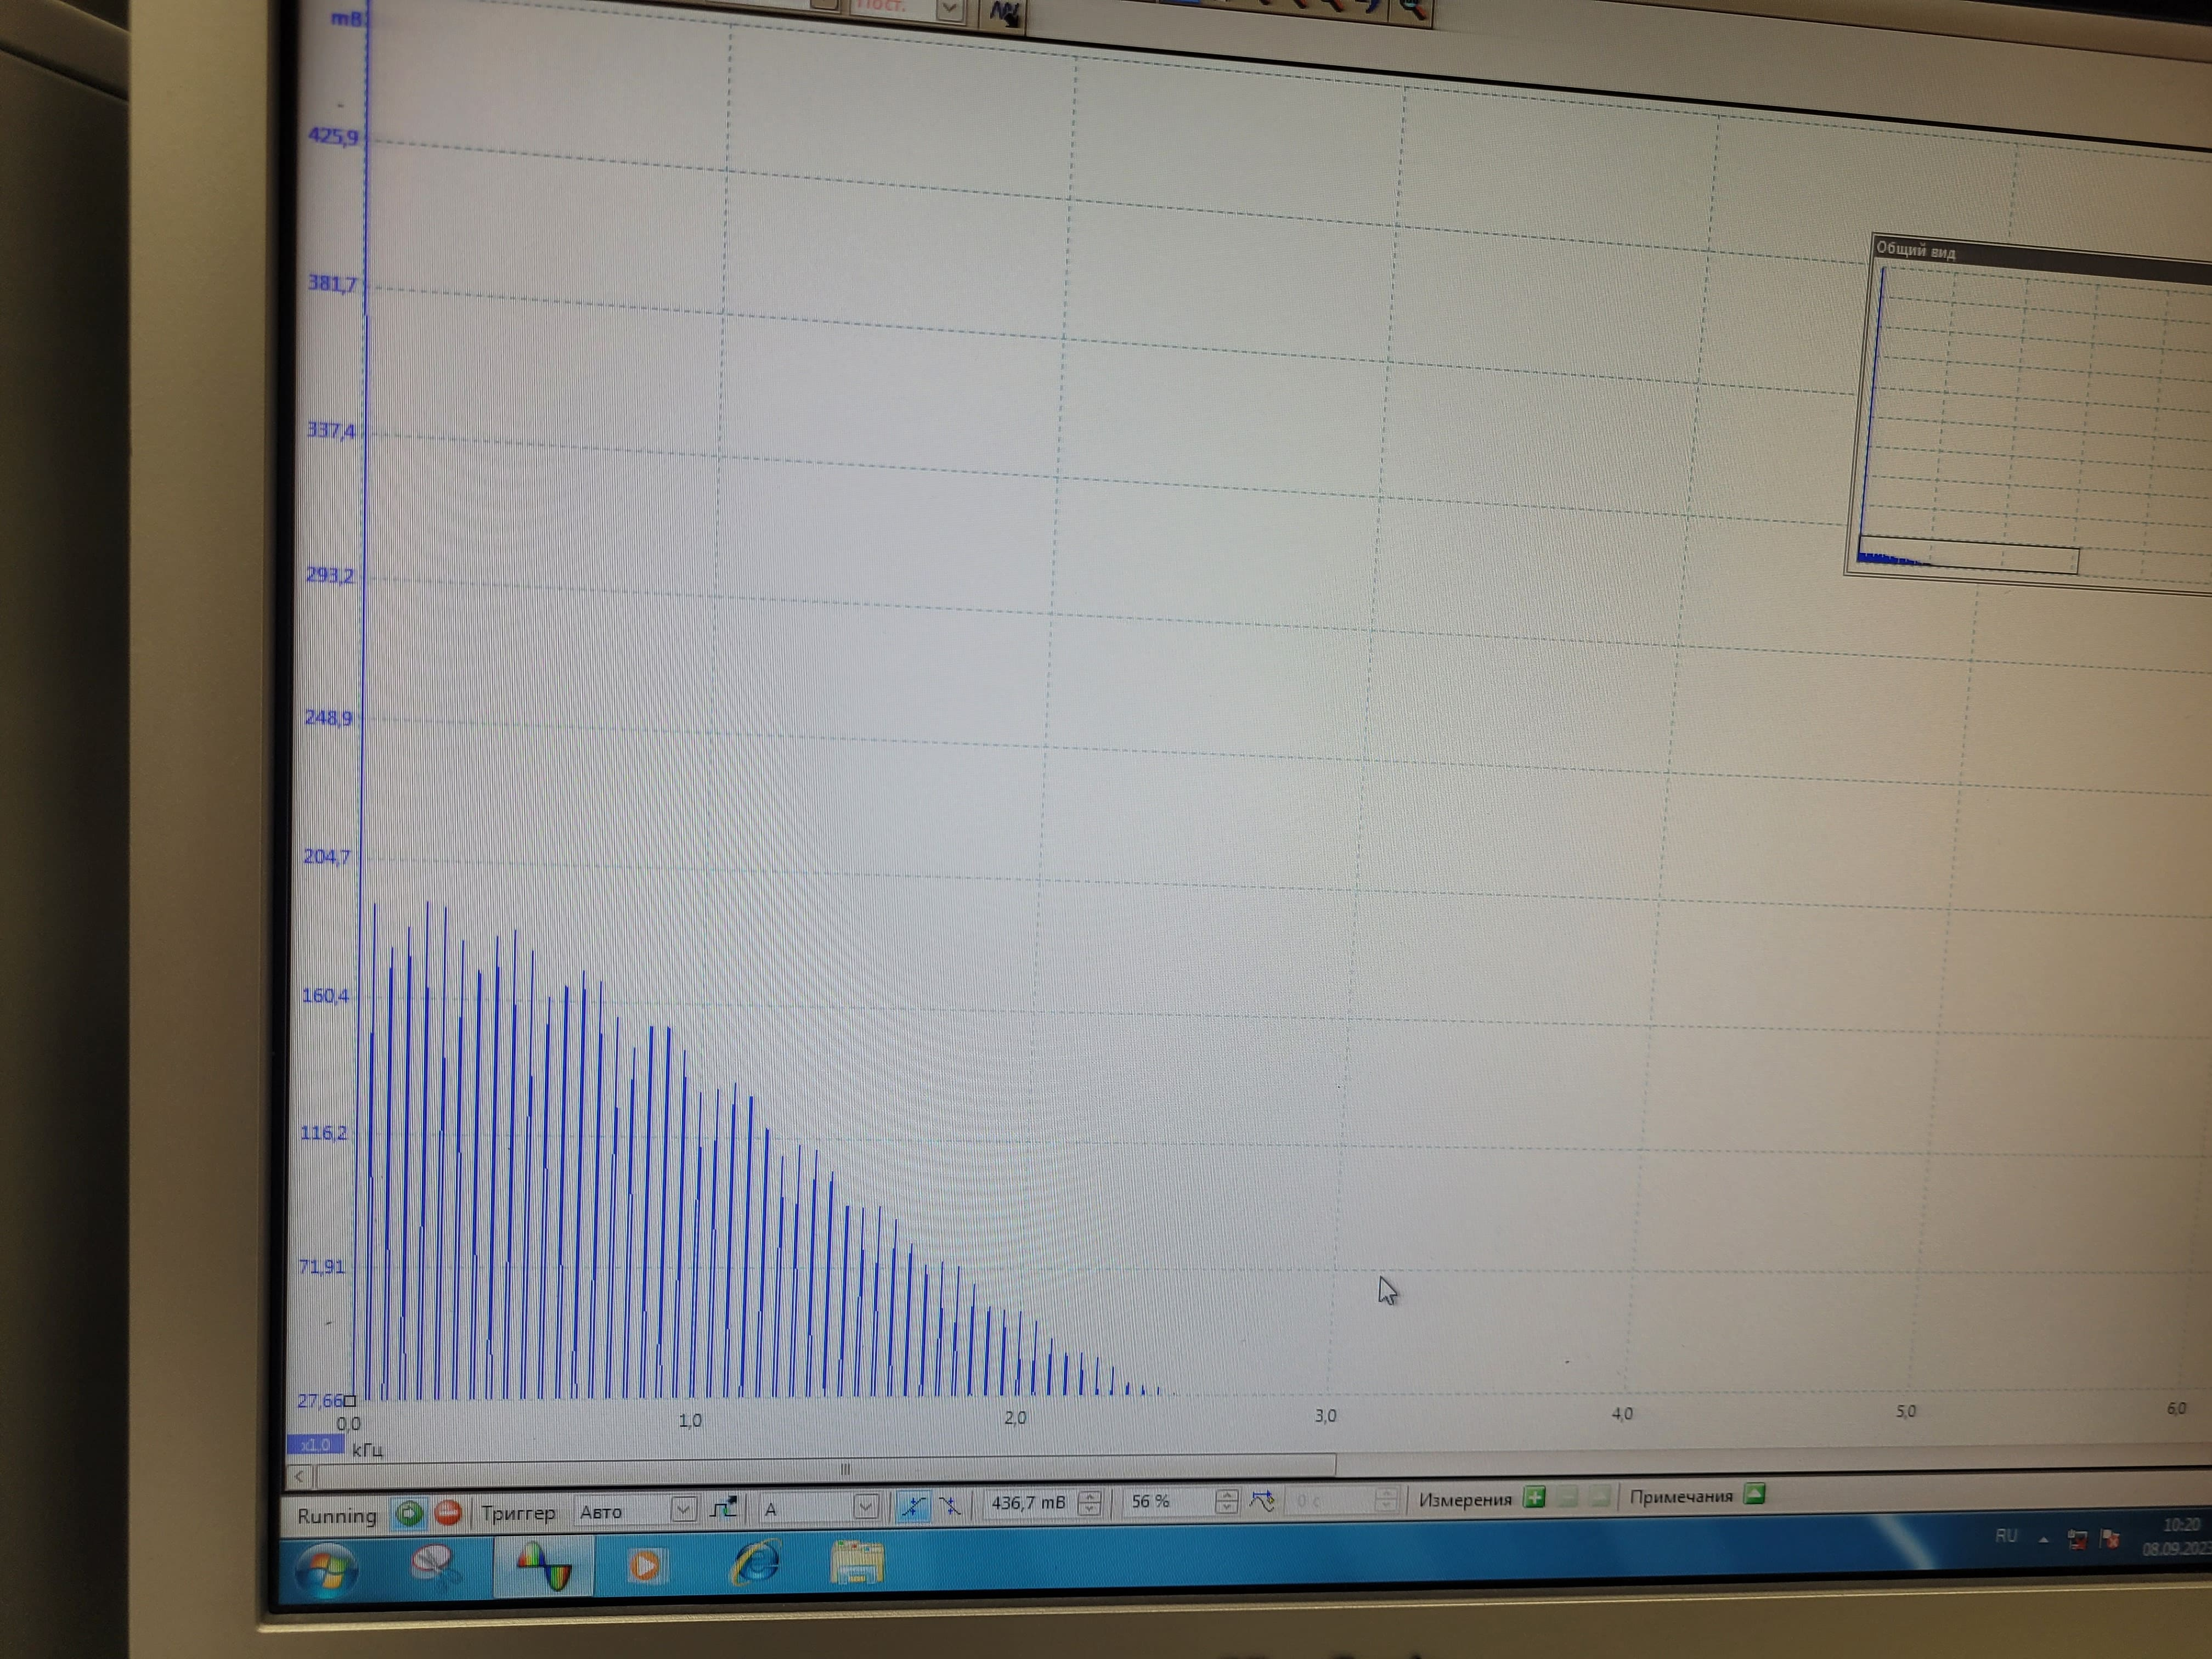
\includegraphics[width=1\linewidth]{V_1k_20T.jpg}} $T$ = 20 мс\\
\end{minipage}
\hfill
\caption{}
\label{ris:experimentalcorrelationsignals}
\end{figure}

\item [\textbf{3.}] Найдём ширину отдельного импульса $\tau$ и его спектра $\Delta \nu$:
\begin{table}[h!]
    \centering
    \begin{tabular}{|c|c|c|}
\hline
$\nu$, кГц & 1 & 2 \\ \hline
$\tau$, мкс & 299.5 & 148.2 \\ \hline
$\frac{\Delta \nu}{2}$, кГц & 1.403 & 2.906 \\ \hline
\end{tabular}
    \caption{}
    \label{table4}
\end{table}
\end{enumerate}

Видно, что соотношение неопределённости выполняется, но численное значение отличается : 
$$\Delta \nu \cdot \tau = 1.403\cdot2\cdot10^3\cdot299.5\cdot10^\text{-6} = 0.84$$

$$\Delta \nu \cdot \tau = 2.906\cdot2\cdot10^3\cdot148.2\cdot10^\text{-6} = 0.86$$


\newpage

\subsection*{Г. Наблюдение спектра амплитудно-модулированного сигнала}


\begin{enumerate}


\item [\textbf{1.}] Настраиваем генератор в режим модулированного по амплитуде синусоидального сигнала с несущей частотой $\nu_0$ = 50 кГц, частотой модуляции $\nu_\text{мод}$ = 2 кГц и глубиной модуляции $m$ = 0.5.

\item [\textbf{2.}] Получаем на экране спектр (Преобразование Фурье) сигнала. Из графика получим $A_{max} = 3.057 \text{мВ}$ и $A_{min} = 1.027 \text{мВ}$ и убедимся в справедливости соотношения $$ m = \frac{A_\text{max} - A_\text{min}}{A_\text{max} + A_\text{min}} = \frac{2.03}{4.084} \approx 0.5 $$
Поскольку мы установили глубину модуляции на $0,5$, а из теории у нас получилась $0,497$, то мы видим, что формула \ref{eq8} верна.

\item [\textbf{3.}]
Изменяя на генераторе глубину модуляции $m$ в диапазоне от 10 \% до 100 \% (всего 6-8 точек), измерим отношение амплитуд боковой и основной 
спектральных линий $a_{\text{бок}}/a_{\text{осн}}$. Построим график зависимости $a_{\text{бок}}/a_{\text{осн}}$ от $m$ и проверим, совпадает ли 
результат с теоретическим.

\begin{center}
\begin{tabular}{|c|c|c|c|c|c|c|c|}
\hline
$m$, \% & 10 & 20 & 30 & 40 & 50 & 80 & 100 \\ \hline
$a_{\text{бок}}$, мВ & 69.02 & 136.3 & 207.1 & 283.2 & 352.2 & 559.2 & 669.0 \\ \hline
\multicolumn{8}{|c|}{$a_{\text{осн}}$ = 1318 мВ} \\ \hline
$a_{\text{бок}}/a_{\text{осн}}$ & 0.05 & 0.10 & 0.16 & 0.21 & 0.27 & 0.42 & 0.51 \\ \hline
\end{tabular}

\textbf{Таблица 3.} Исследование зависимости $a_{\text{бок}}/a_{\text{осн}}$ от $m$.
\end{center}
\begin{figure}[h]
    \centering
    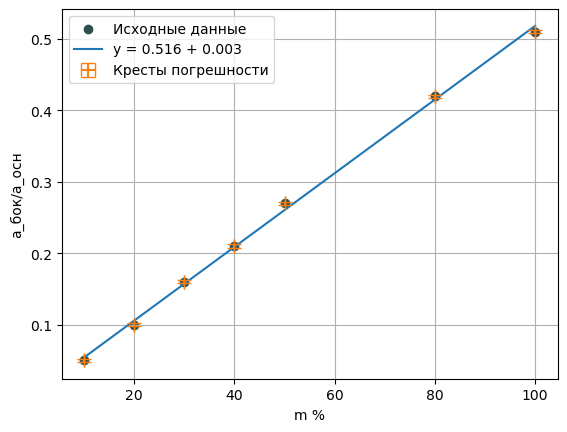
\includegraphics[width=0.7\linewidth]{grafic3.png}
    \caption{Зависимость $a_{\text{бок}}/a_{\text{осн}}$ от $m$}
    \label{grafic3}
\end{figure}
Построим график $\frac{a_{\text{бок}}}{a_{\text{осн}}}(m)$. Используя МНК, получим $k=0.516x\pm0,00007$, что подтверждает $\frac{a_{\text{бок}}}{a_{\text{осн}}}=\frac{m}{2}$, т.е. совпадает с теоретическим предсказанием. График приведён на рис.\ref{grafic3}.




\end{enumerate}








\newpage



\subsection*{Д. Наблюдение спектра сигнала, модулированного по фазе}



\begin{enumerate}


\item [\textbf{1.}] Настраиваем генератор в режим модулированного по фазе синусоидального сигнала с несущей частотой $\nu_0$ = 50 кГц, частотой модуляции $\nu_\text{мод}$ = 2 кГц и максимальным отклонением (глубиной модуляцией) $\varphi$ = 10$\degree$.

\item [\textbf{2.}] Получаем на экране спектр (Преобразование Фурье) сигнала.

\begin{figure}[h]
\begin{minipage}[h]{0.44\linewidth}
\center{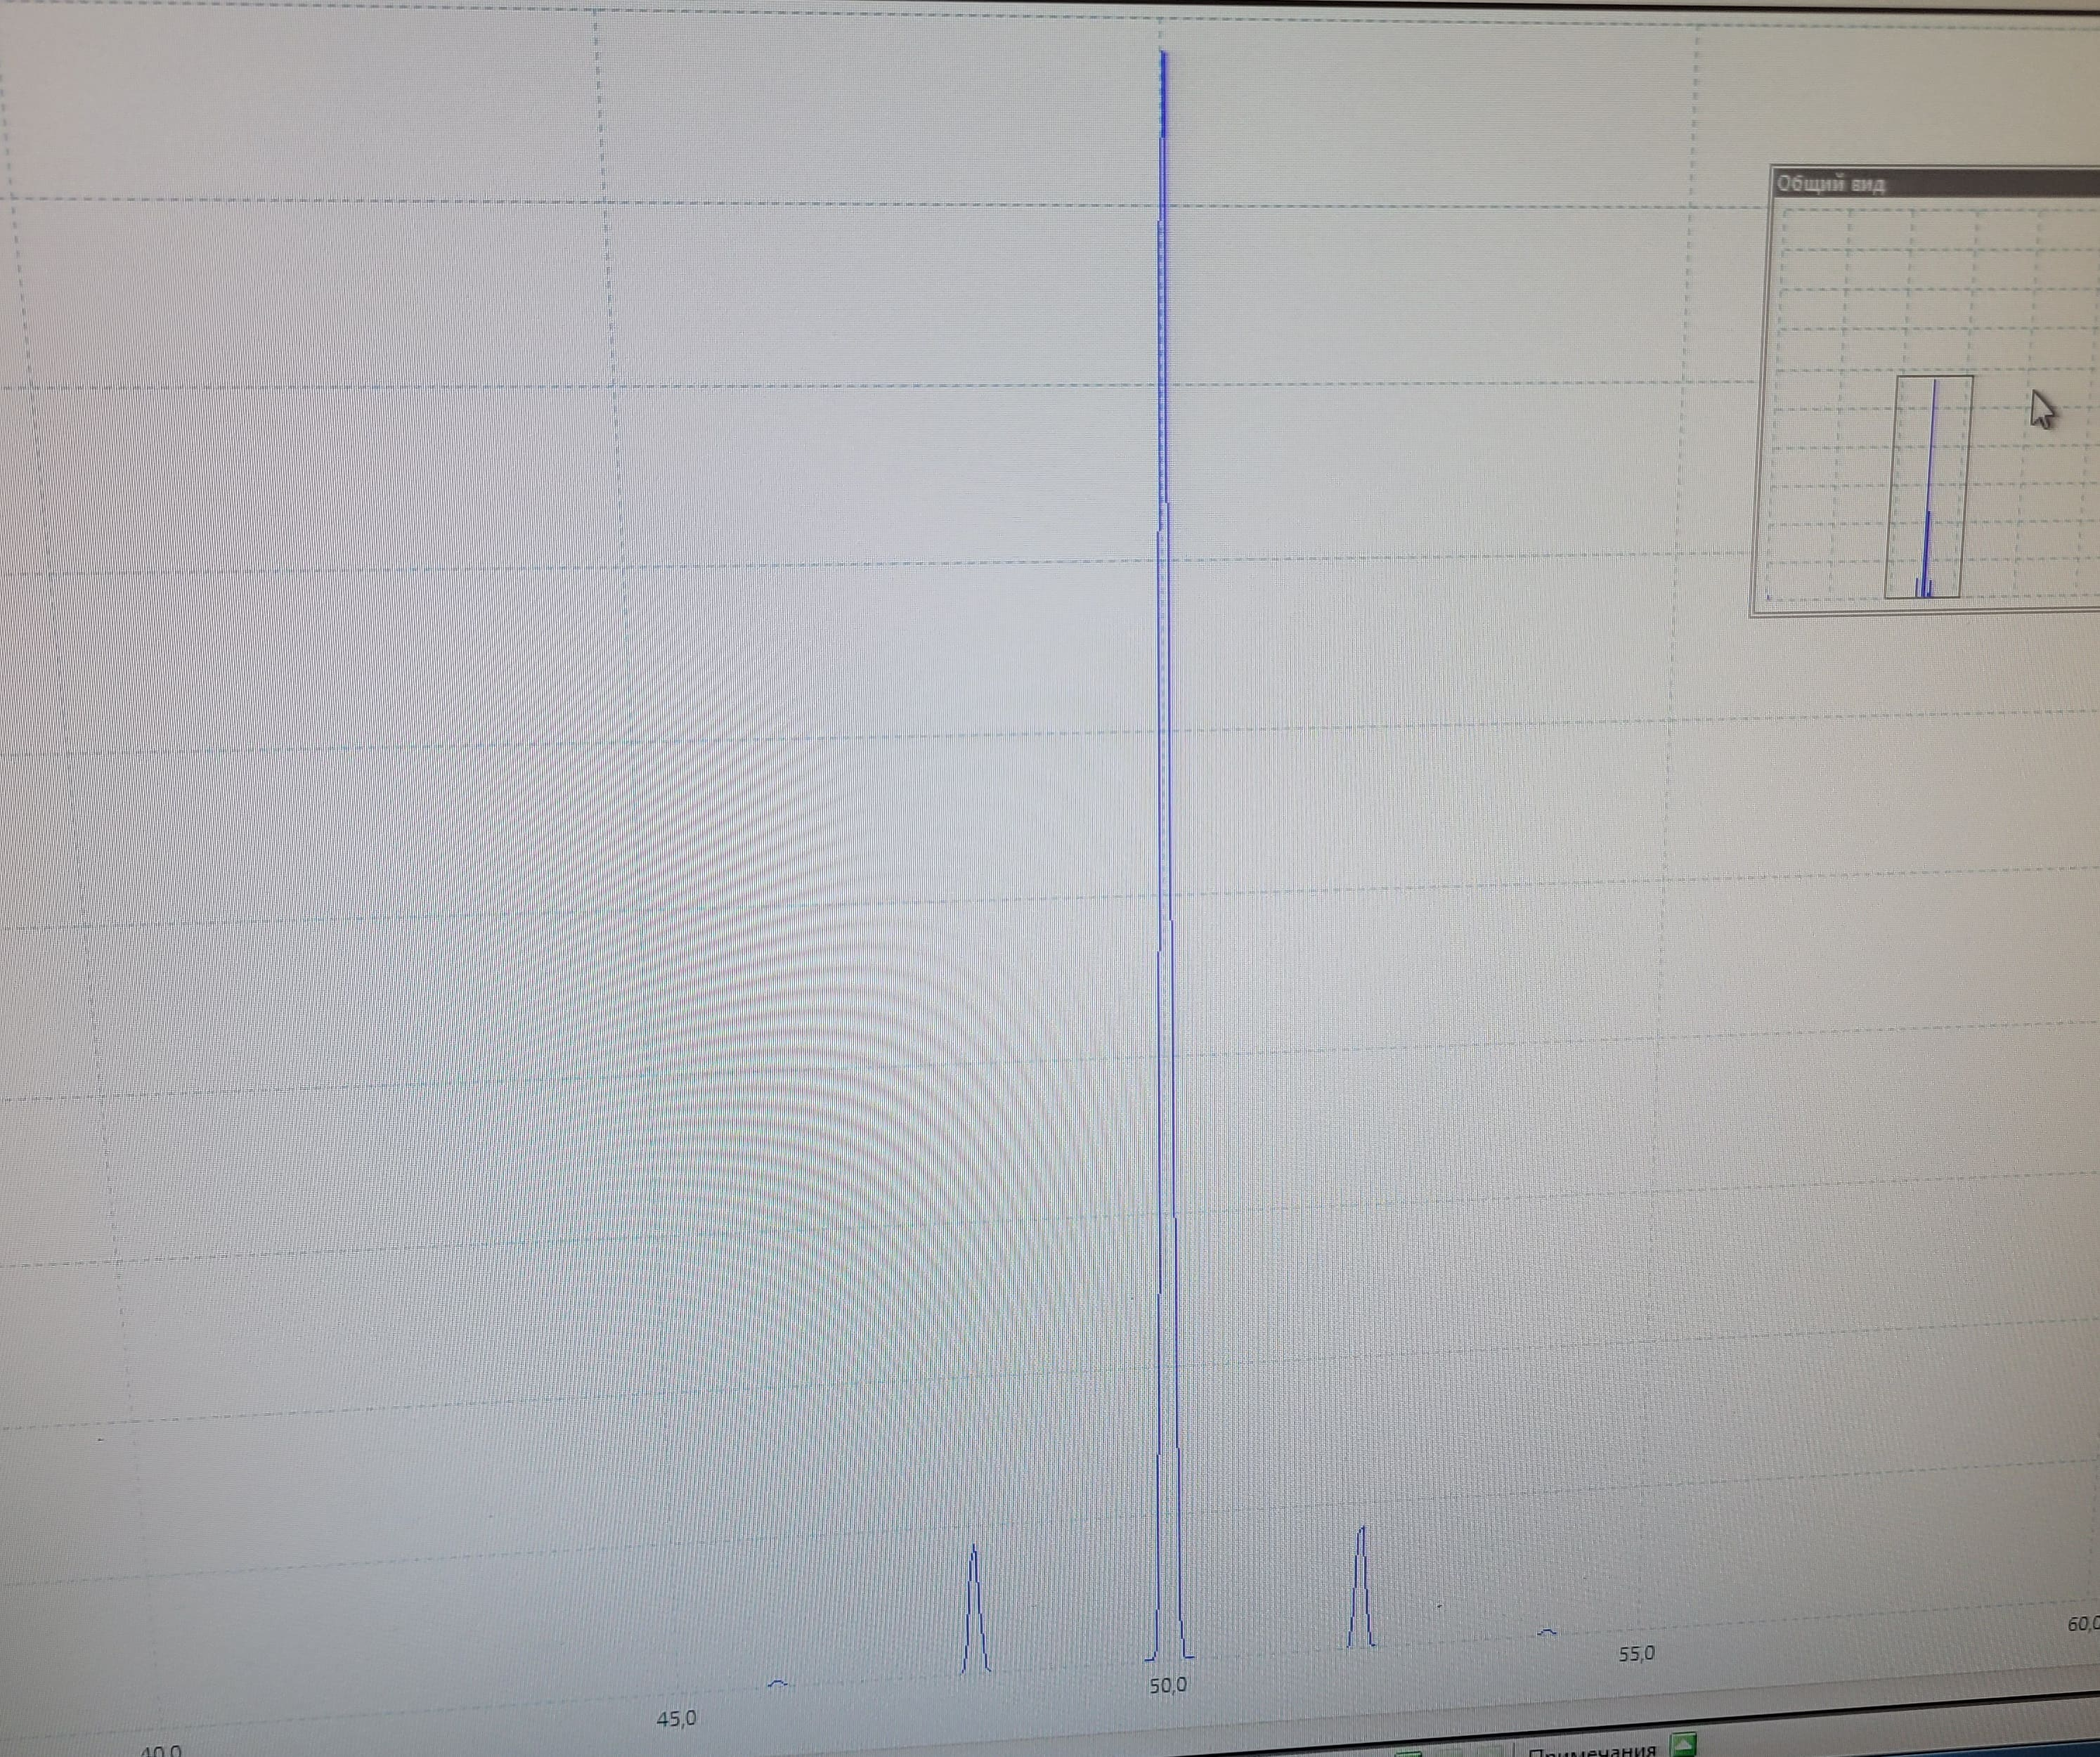
\includegraphics[width=1\linewidth]{D_50k_2k_10f.jpg}} $\nu_0$ = 50 кГц, $\nu_\text{мод}$ = 2 кГц, $\varphi$ = 10$\degree$  \\
\end{minipage}
\hfill
\begin{minipage}[h]{0.44\linewidth}
\center{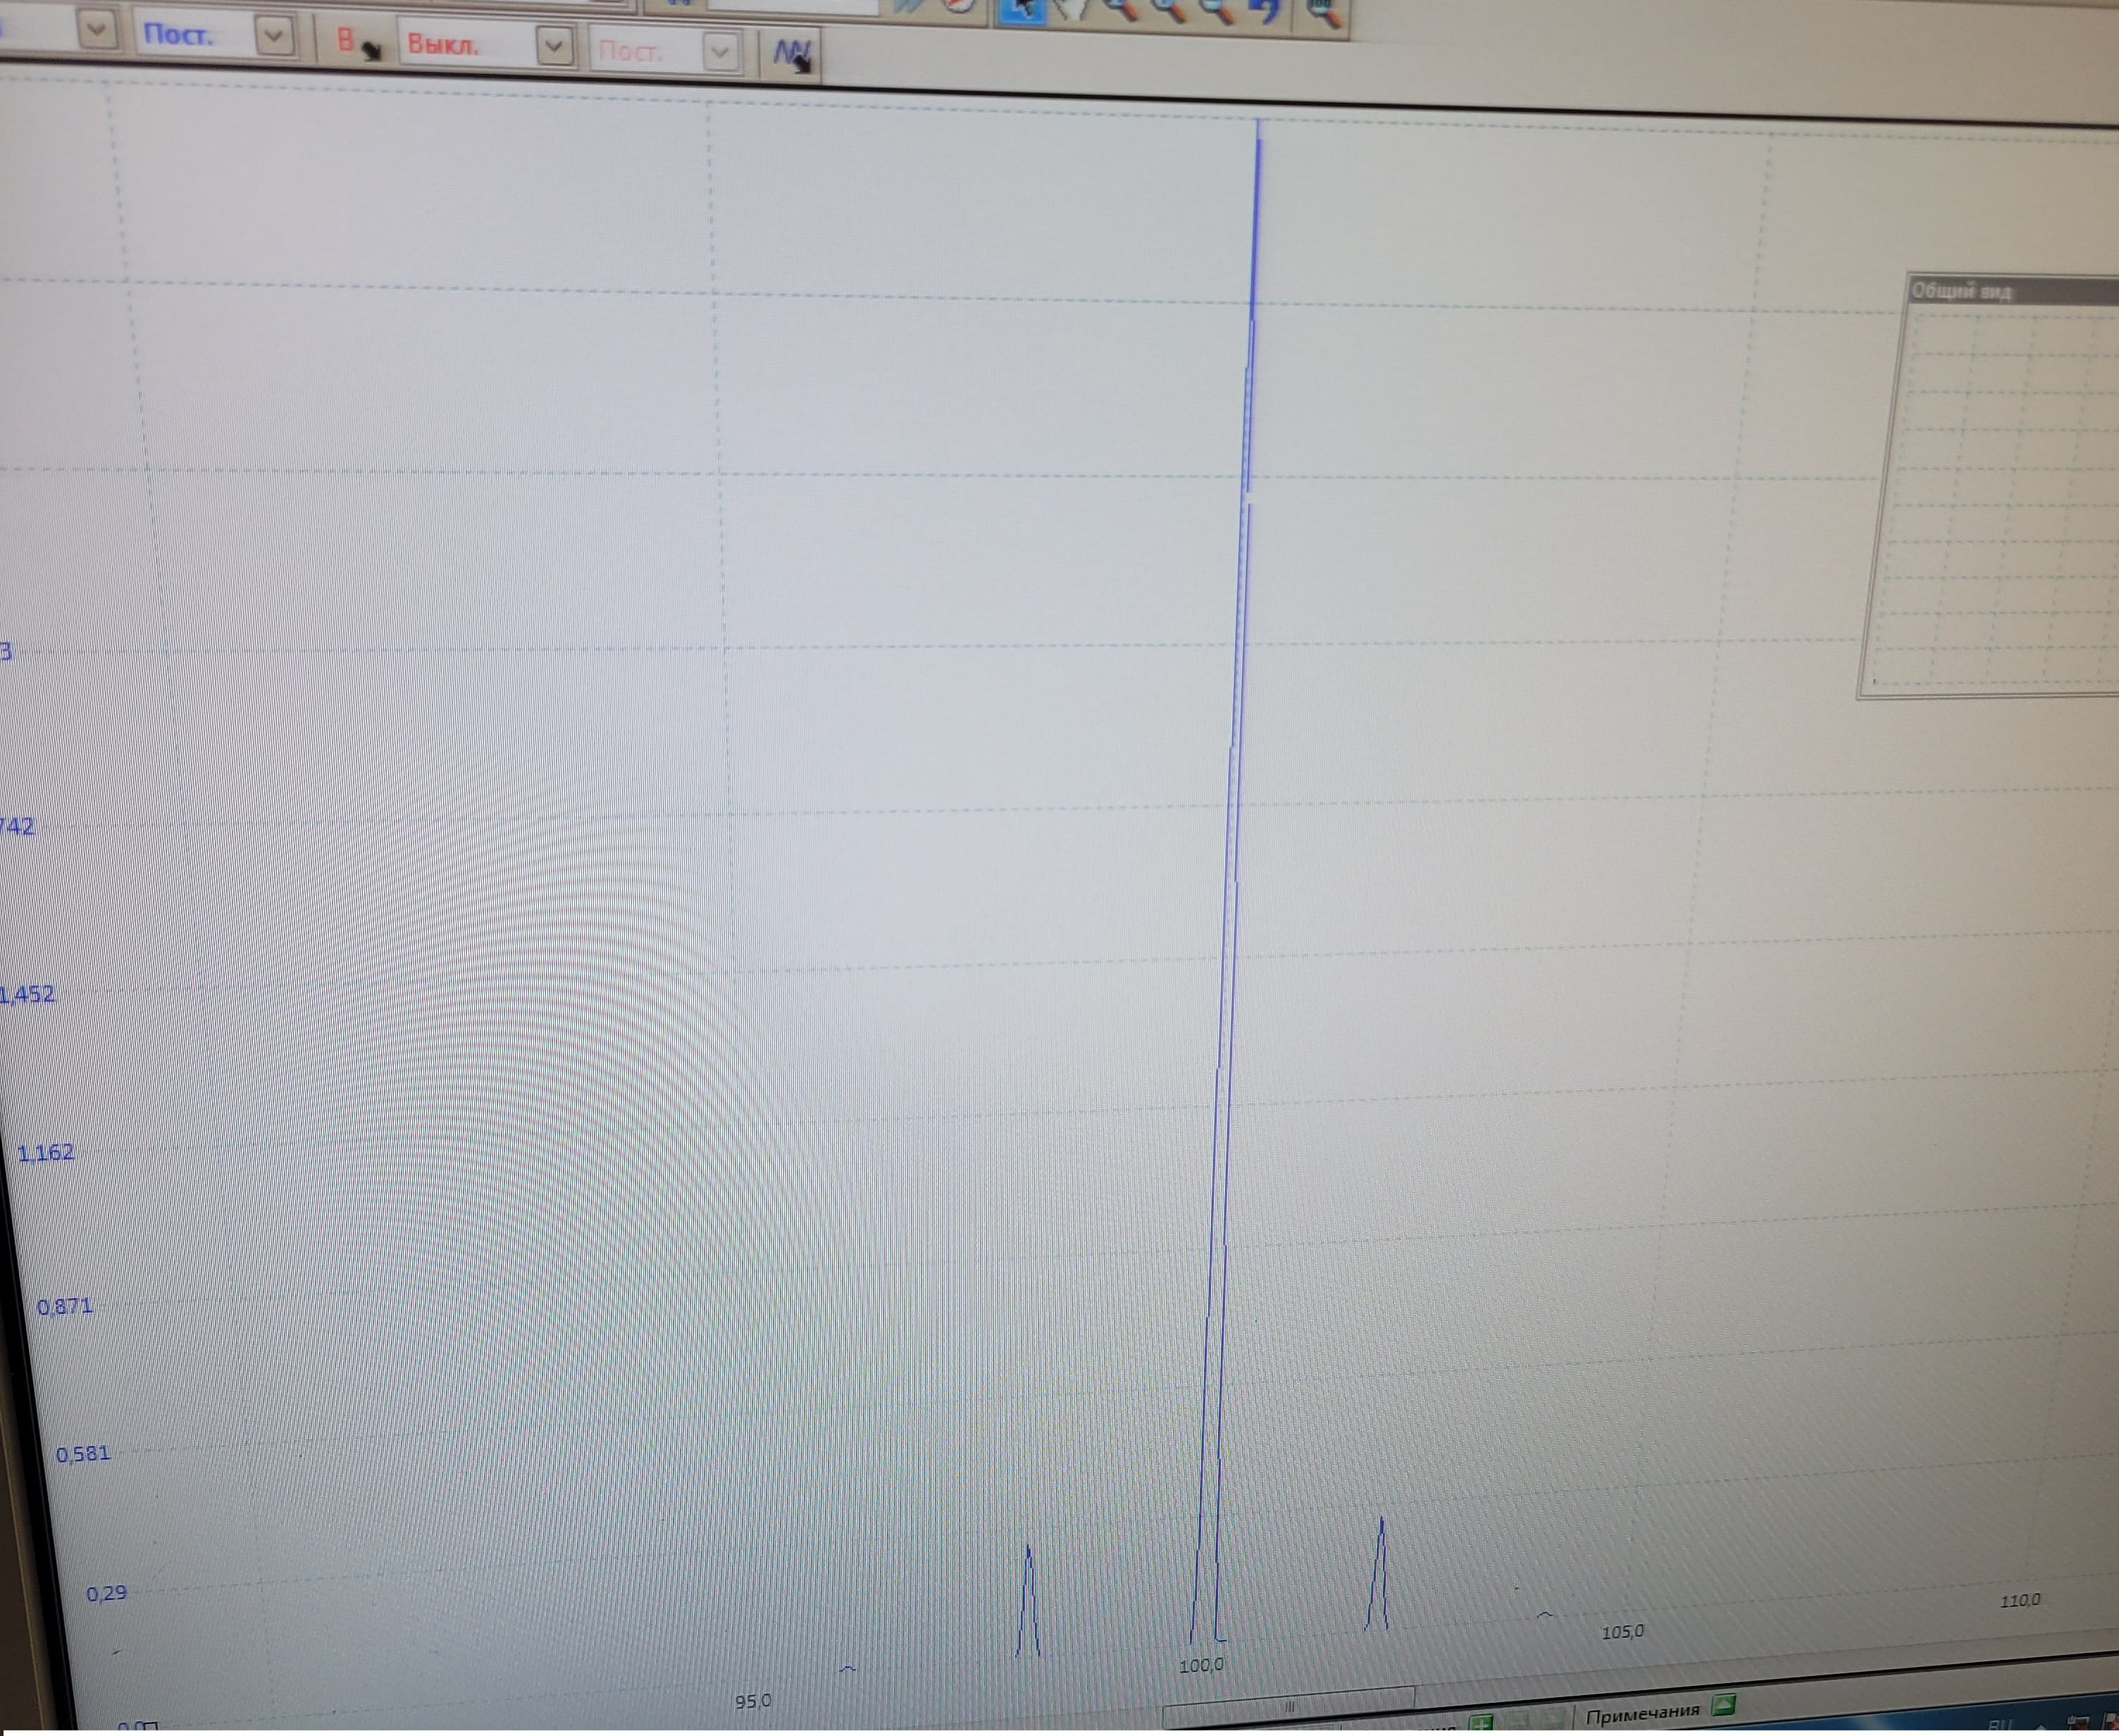
\includegraphics[width=1\linewidth]{D_100k_2k_10f.jpg}} \\  $\nu_0$ = 100 кГц, $\nu_\text{мод}$ = 2 кГц, $\varphi$ = 10$\degree$   
\end{minipage}
\vfill
\begin{minipage}[h]{0.44\linewidth}
\center{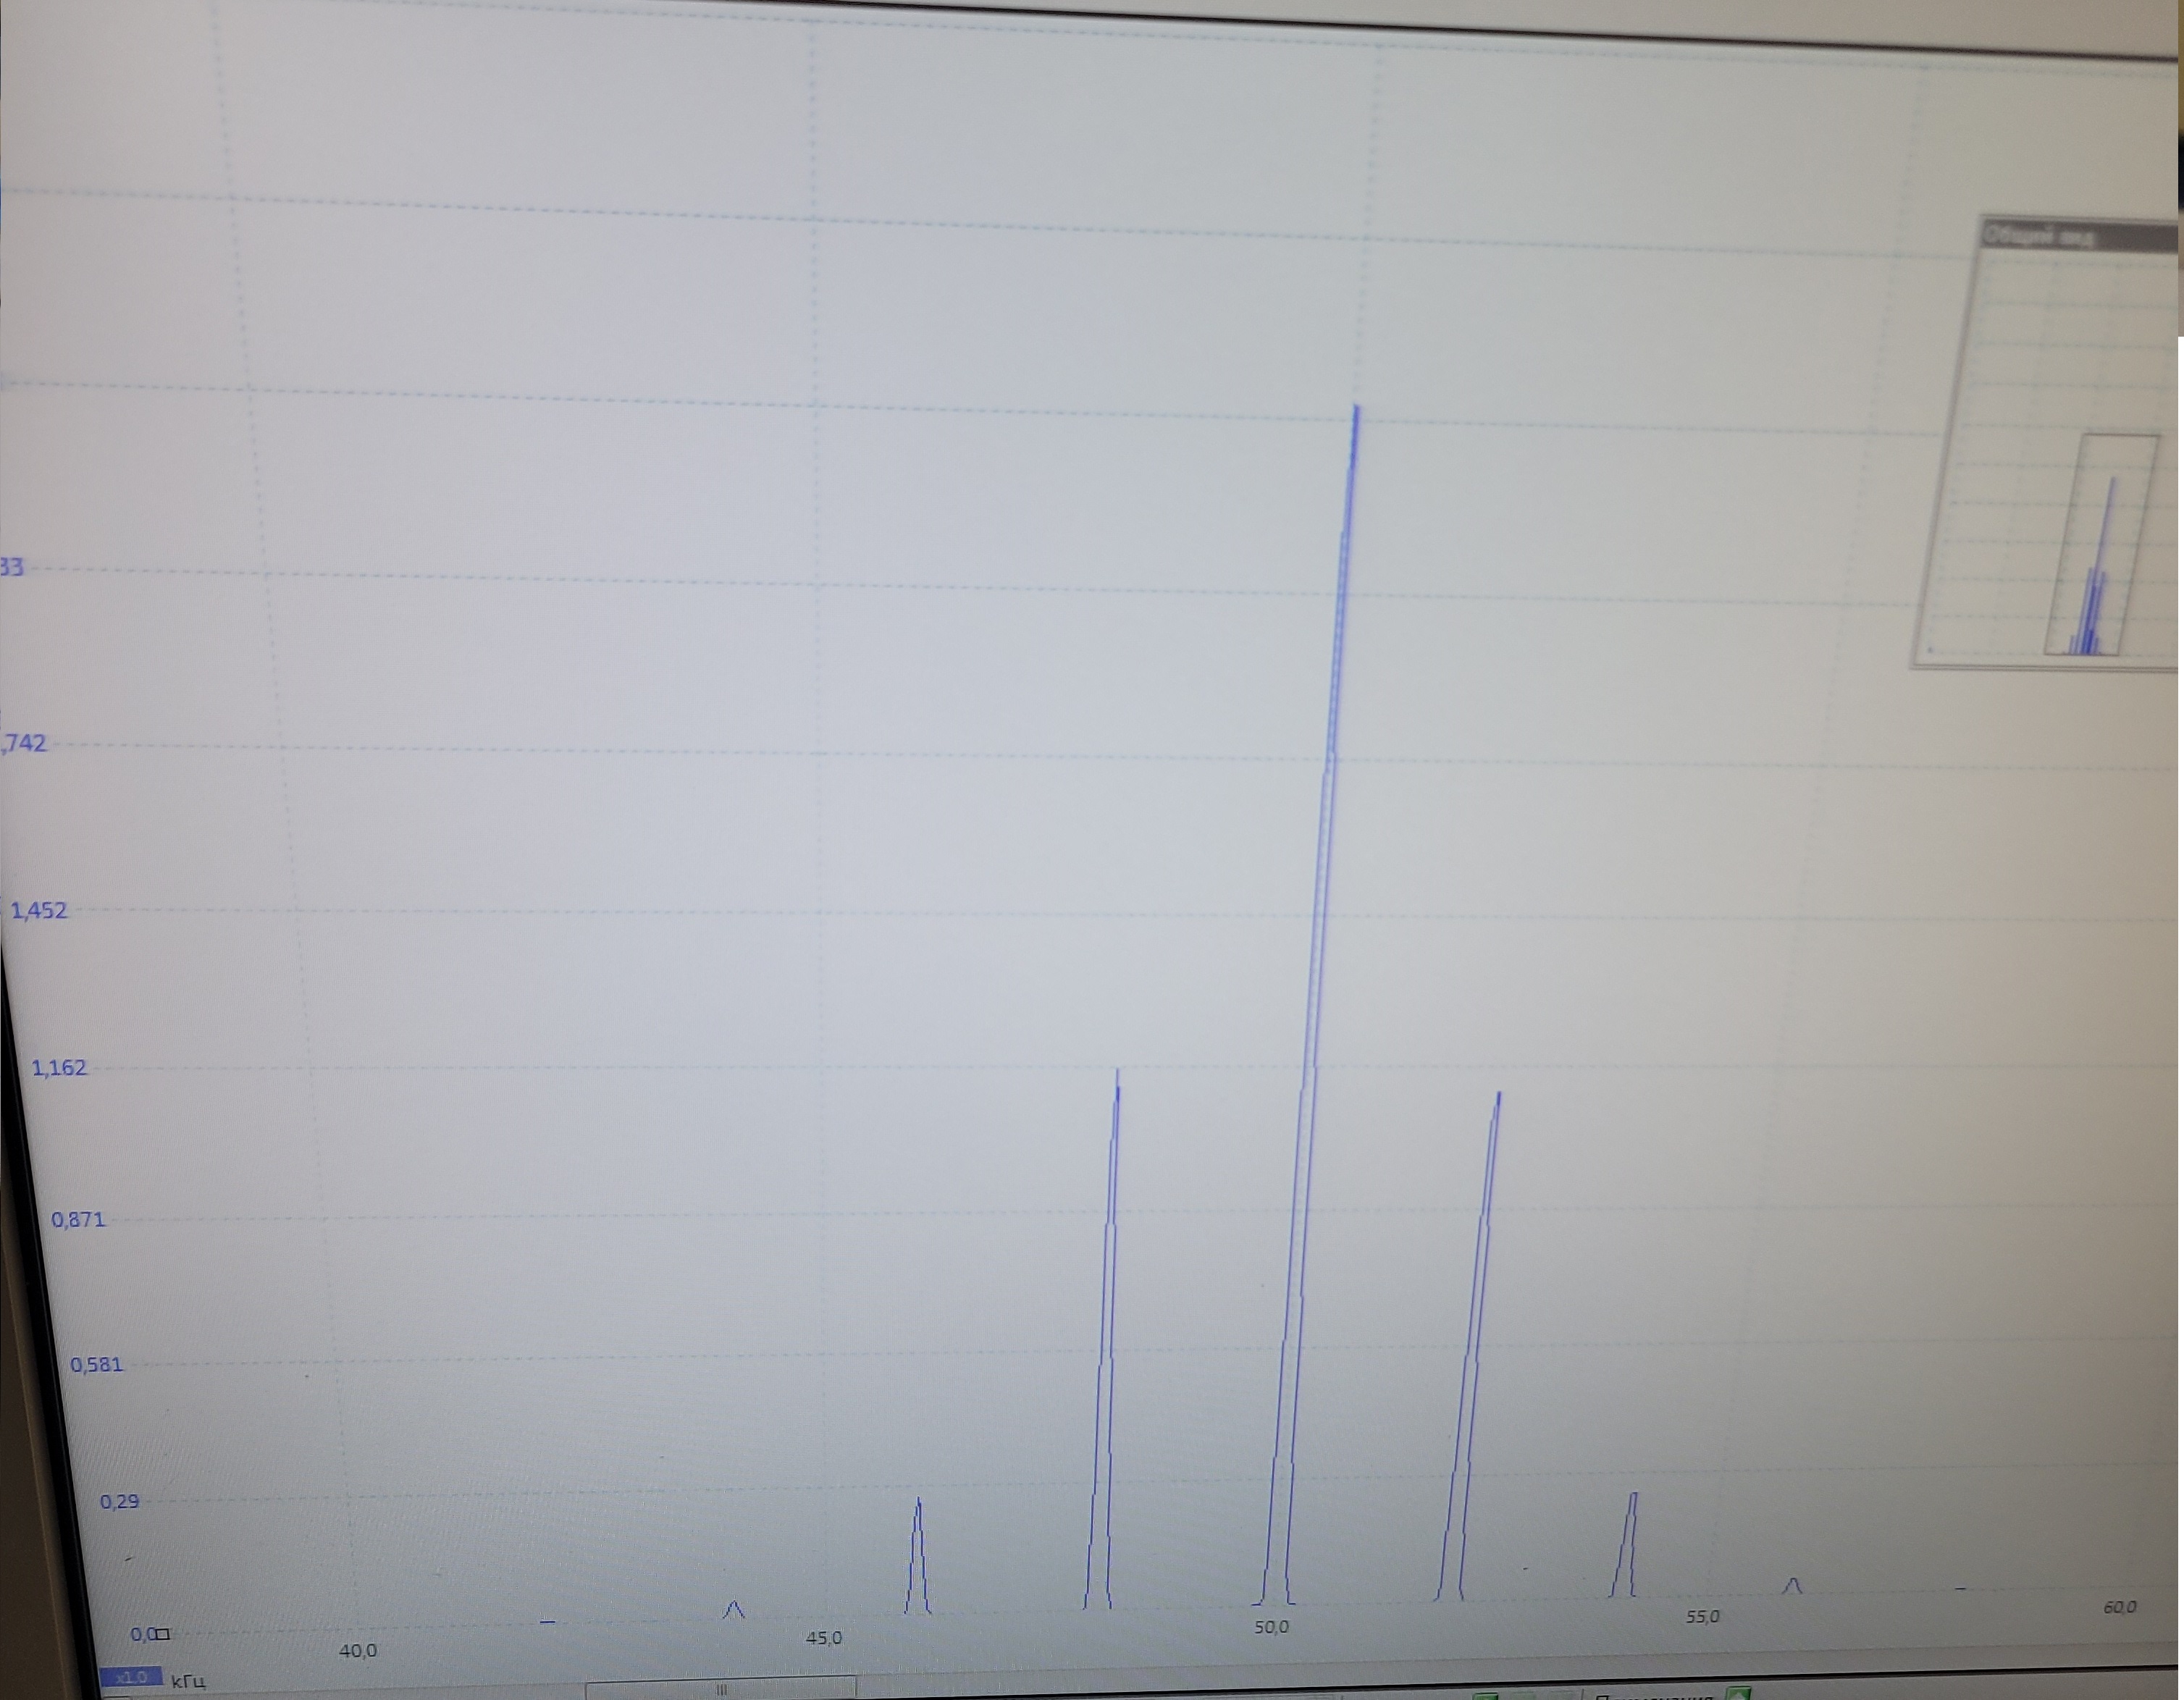
\includegraphics[width=1\linewidth]{D_50k_2k_50f.jpg}} $\nu_0$ = 50 кГц, $\nu_\text{мод}$ = 2 кГц, $\varphi$ = 50$\degree$   \\
\end{minipage}
\hfill
\begin{minipage}[h]{0.44\linewidth}
\center{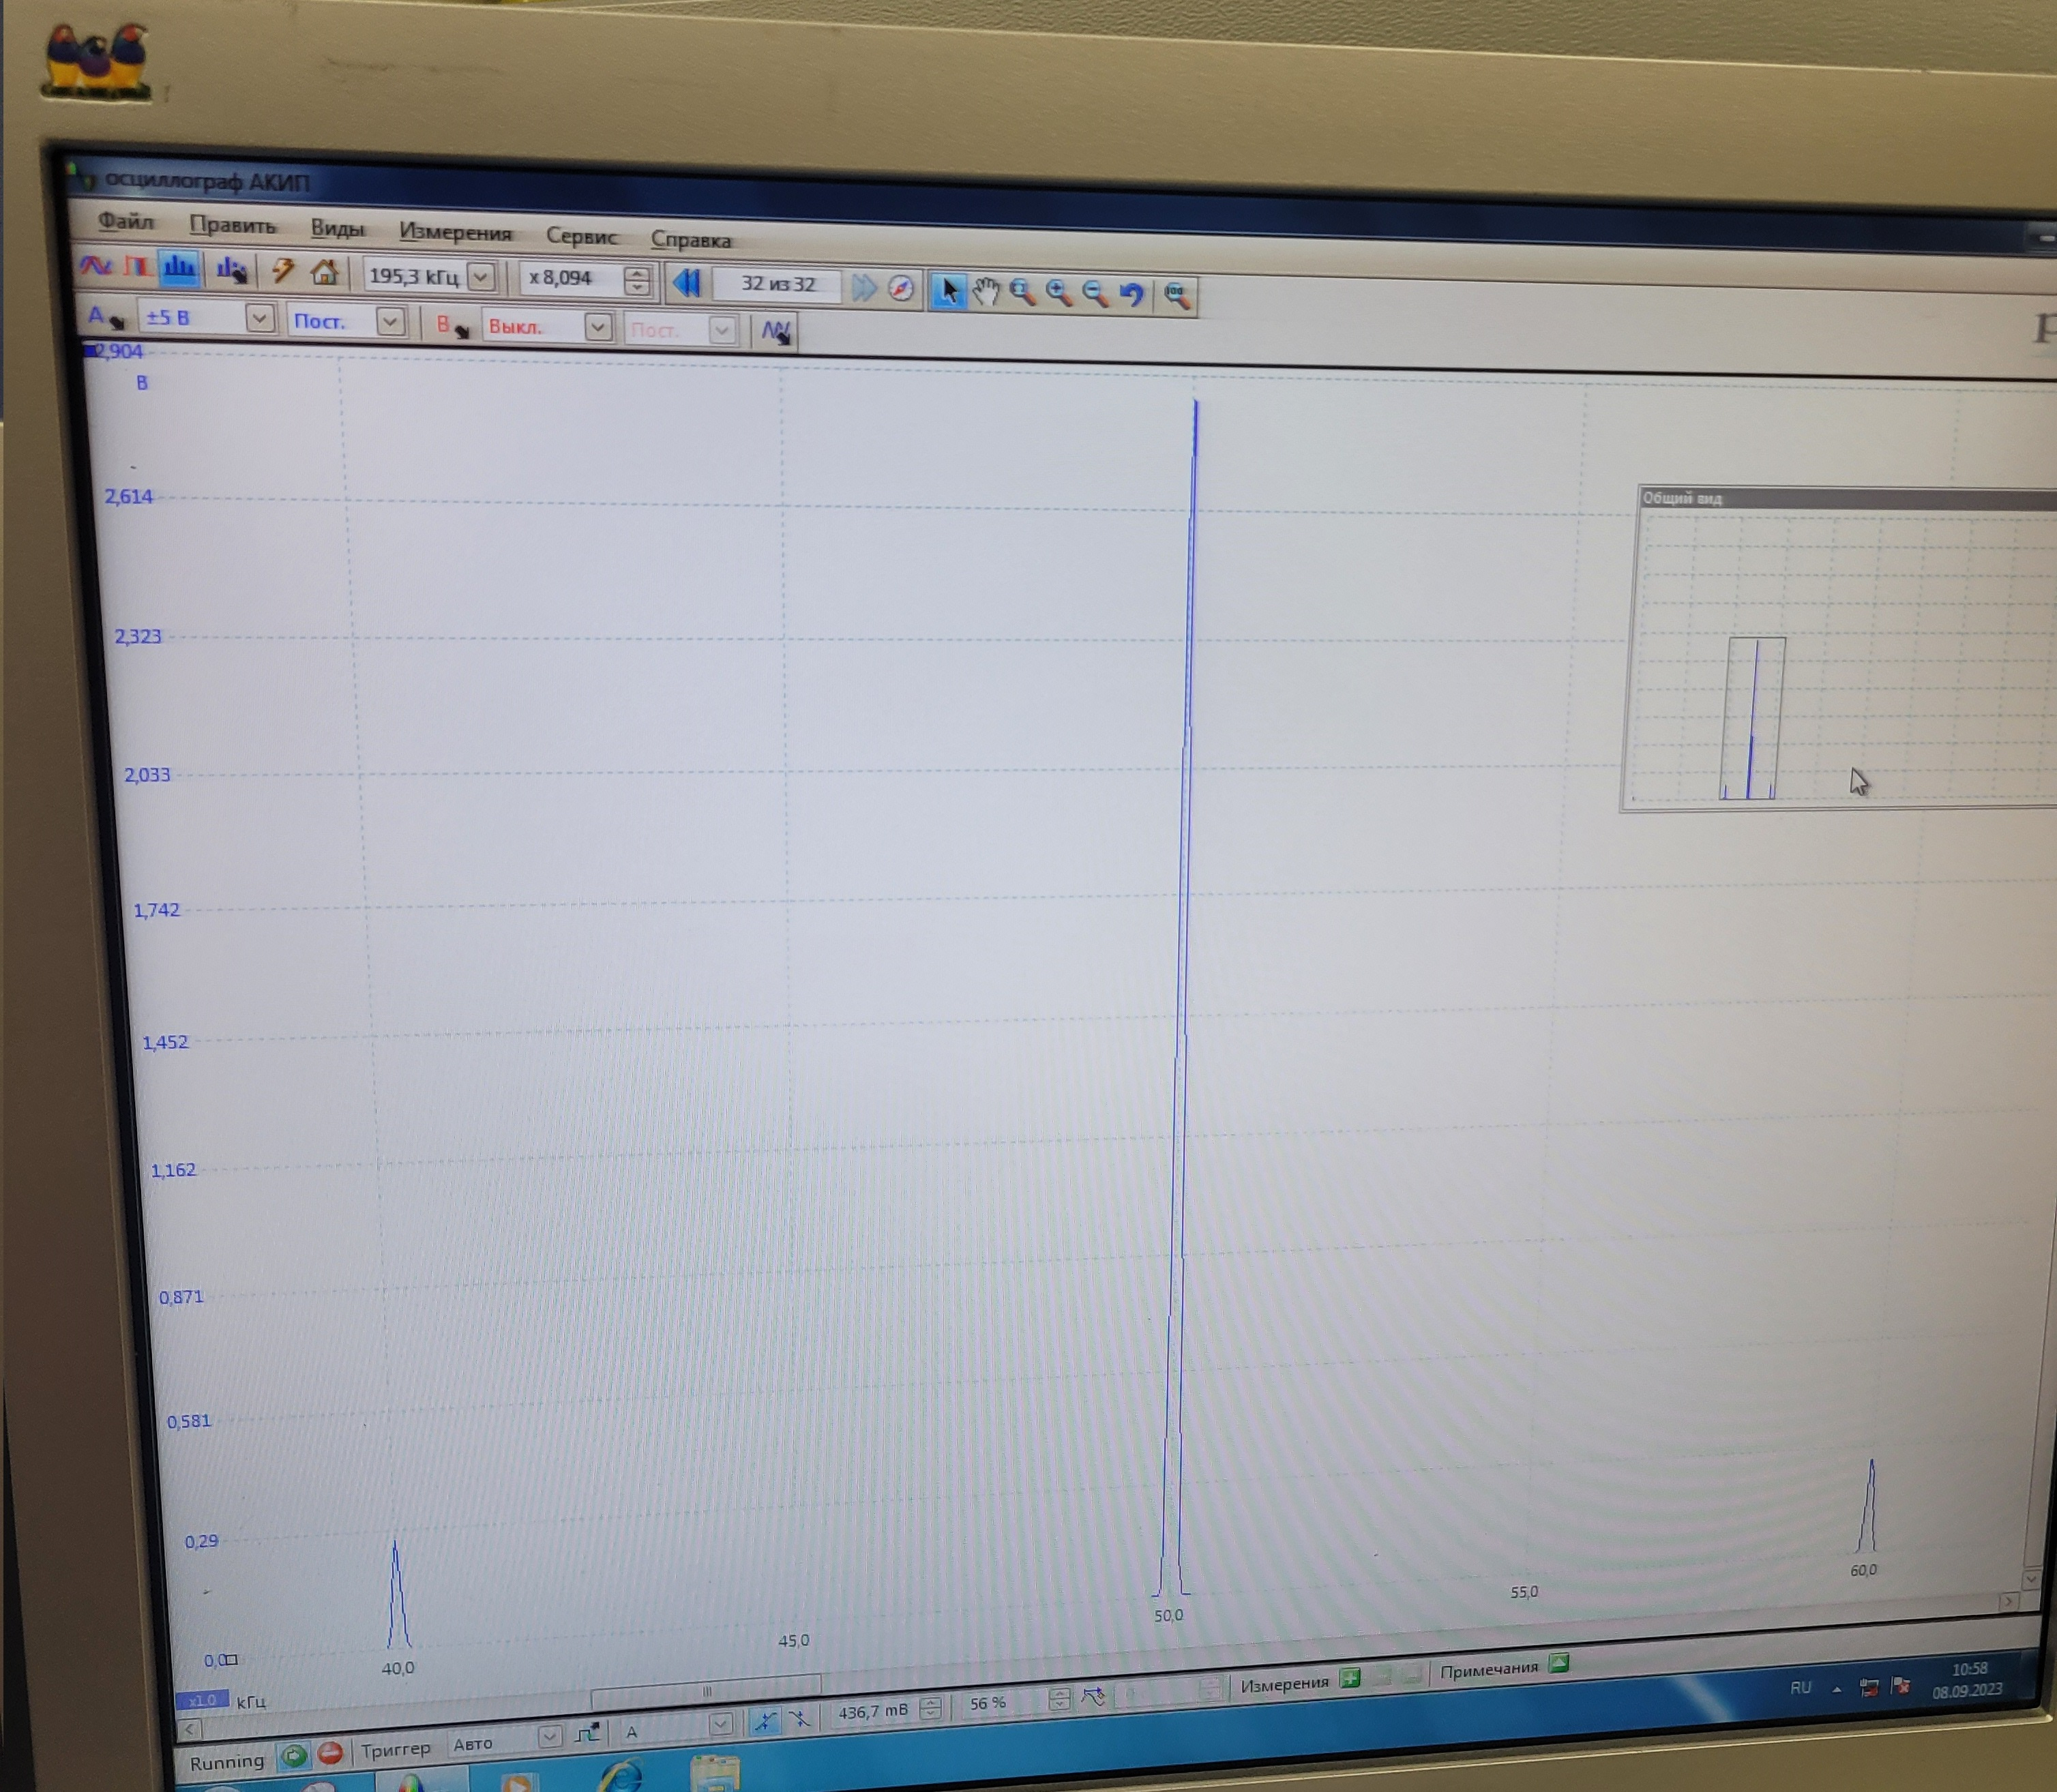
\includegraphics[width=1\linewidth]{D_50k_10k_10f.jpg}} $\nu_0$ = 50 кГц, $\nu_\text{мод}$ = 10 кГц, $\varphi$ = 10$\degree$  \\
\end{minipage}
\vfill
\caption{}
\label{ris:experimentalcorrelationsignals}
\end{figure}


\newpage




\begin{figure}[h]
\begin{minipage}[h]{0.44\linewidth}
\center{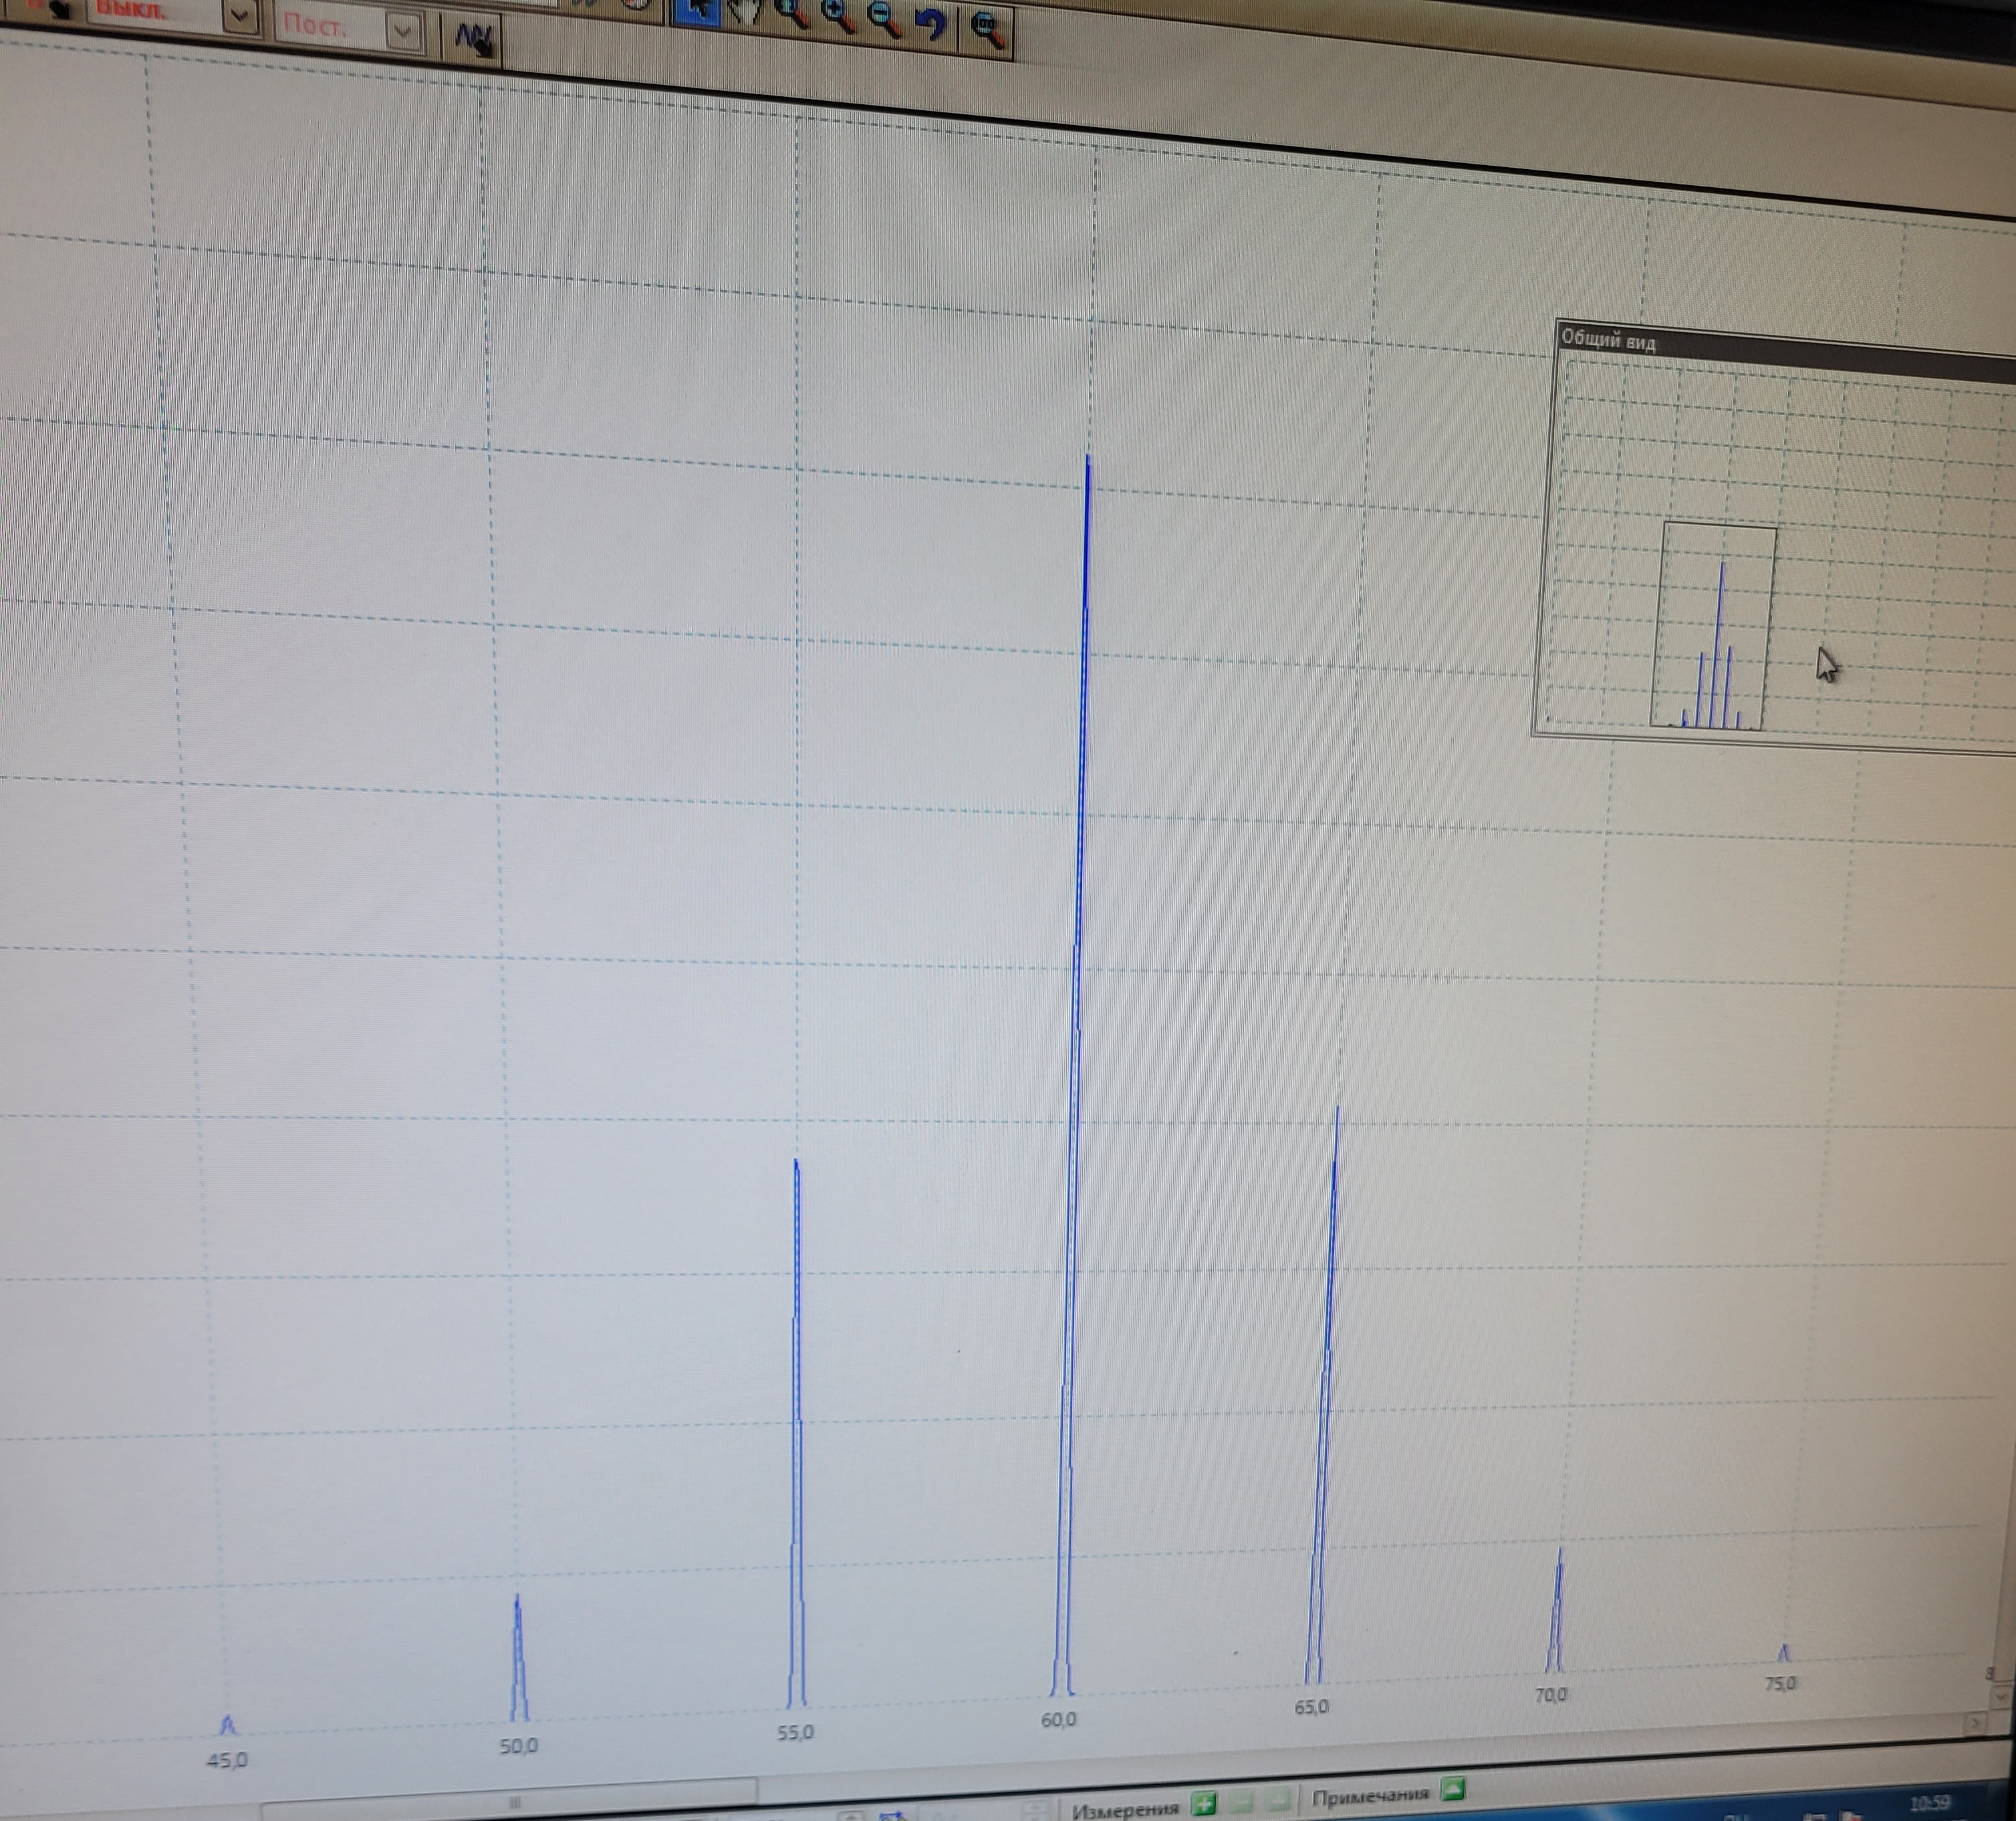
\includegraphics[width=1\linewidth]{D_60k_5k_50f.jpg}} $\nu_0$ = 60 кГц, $\nu_\text{мод}$ = 5 кГц, $\varphi$ = 50$\degree$  \\
\end{minipage}
\label{ris:experimentalcorrelationsignals}
\end{figure}




\end{enumerate}


\newpage










\subsection*{Е. Изучение фильтрации сигналов}



\begin{enumerate}


\item [\textbf{1.}] Подключаем $RC$ цепочку с сопротивлением $R = 3$ кОм и ёмкостью $C = 1000$ пФ. Получаем характерное время $\tau_{RC} = RC = 3 $ мкс. Подаём на вход $RC$-цепочки последовательность прямоугольных импульсов с периодом повторения $T \sim \tau_{RC}$.


\item [\textbf{2.}] Получаем на экране спектр (Преобразование Фурье) сигнала.

\begin{figure}[h]
\begin{minipage}[h]{0.44\linewidth}
\center{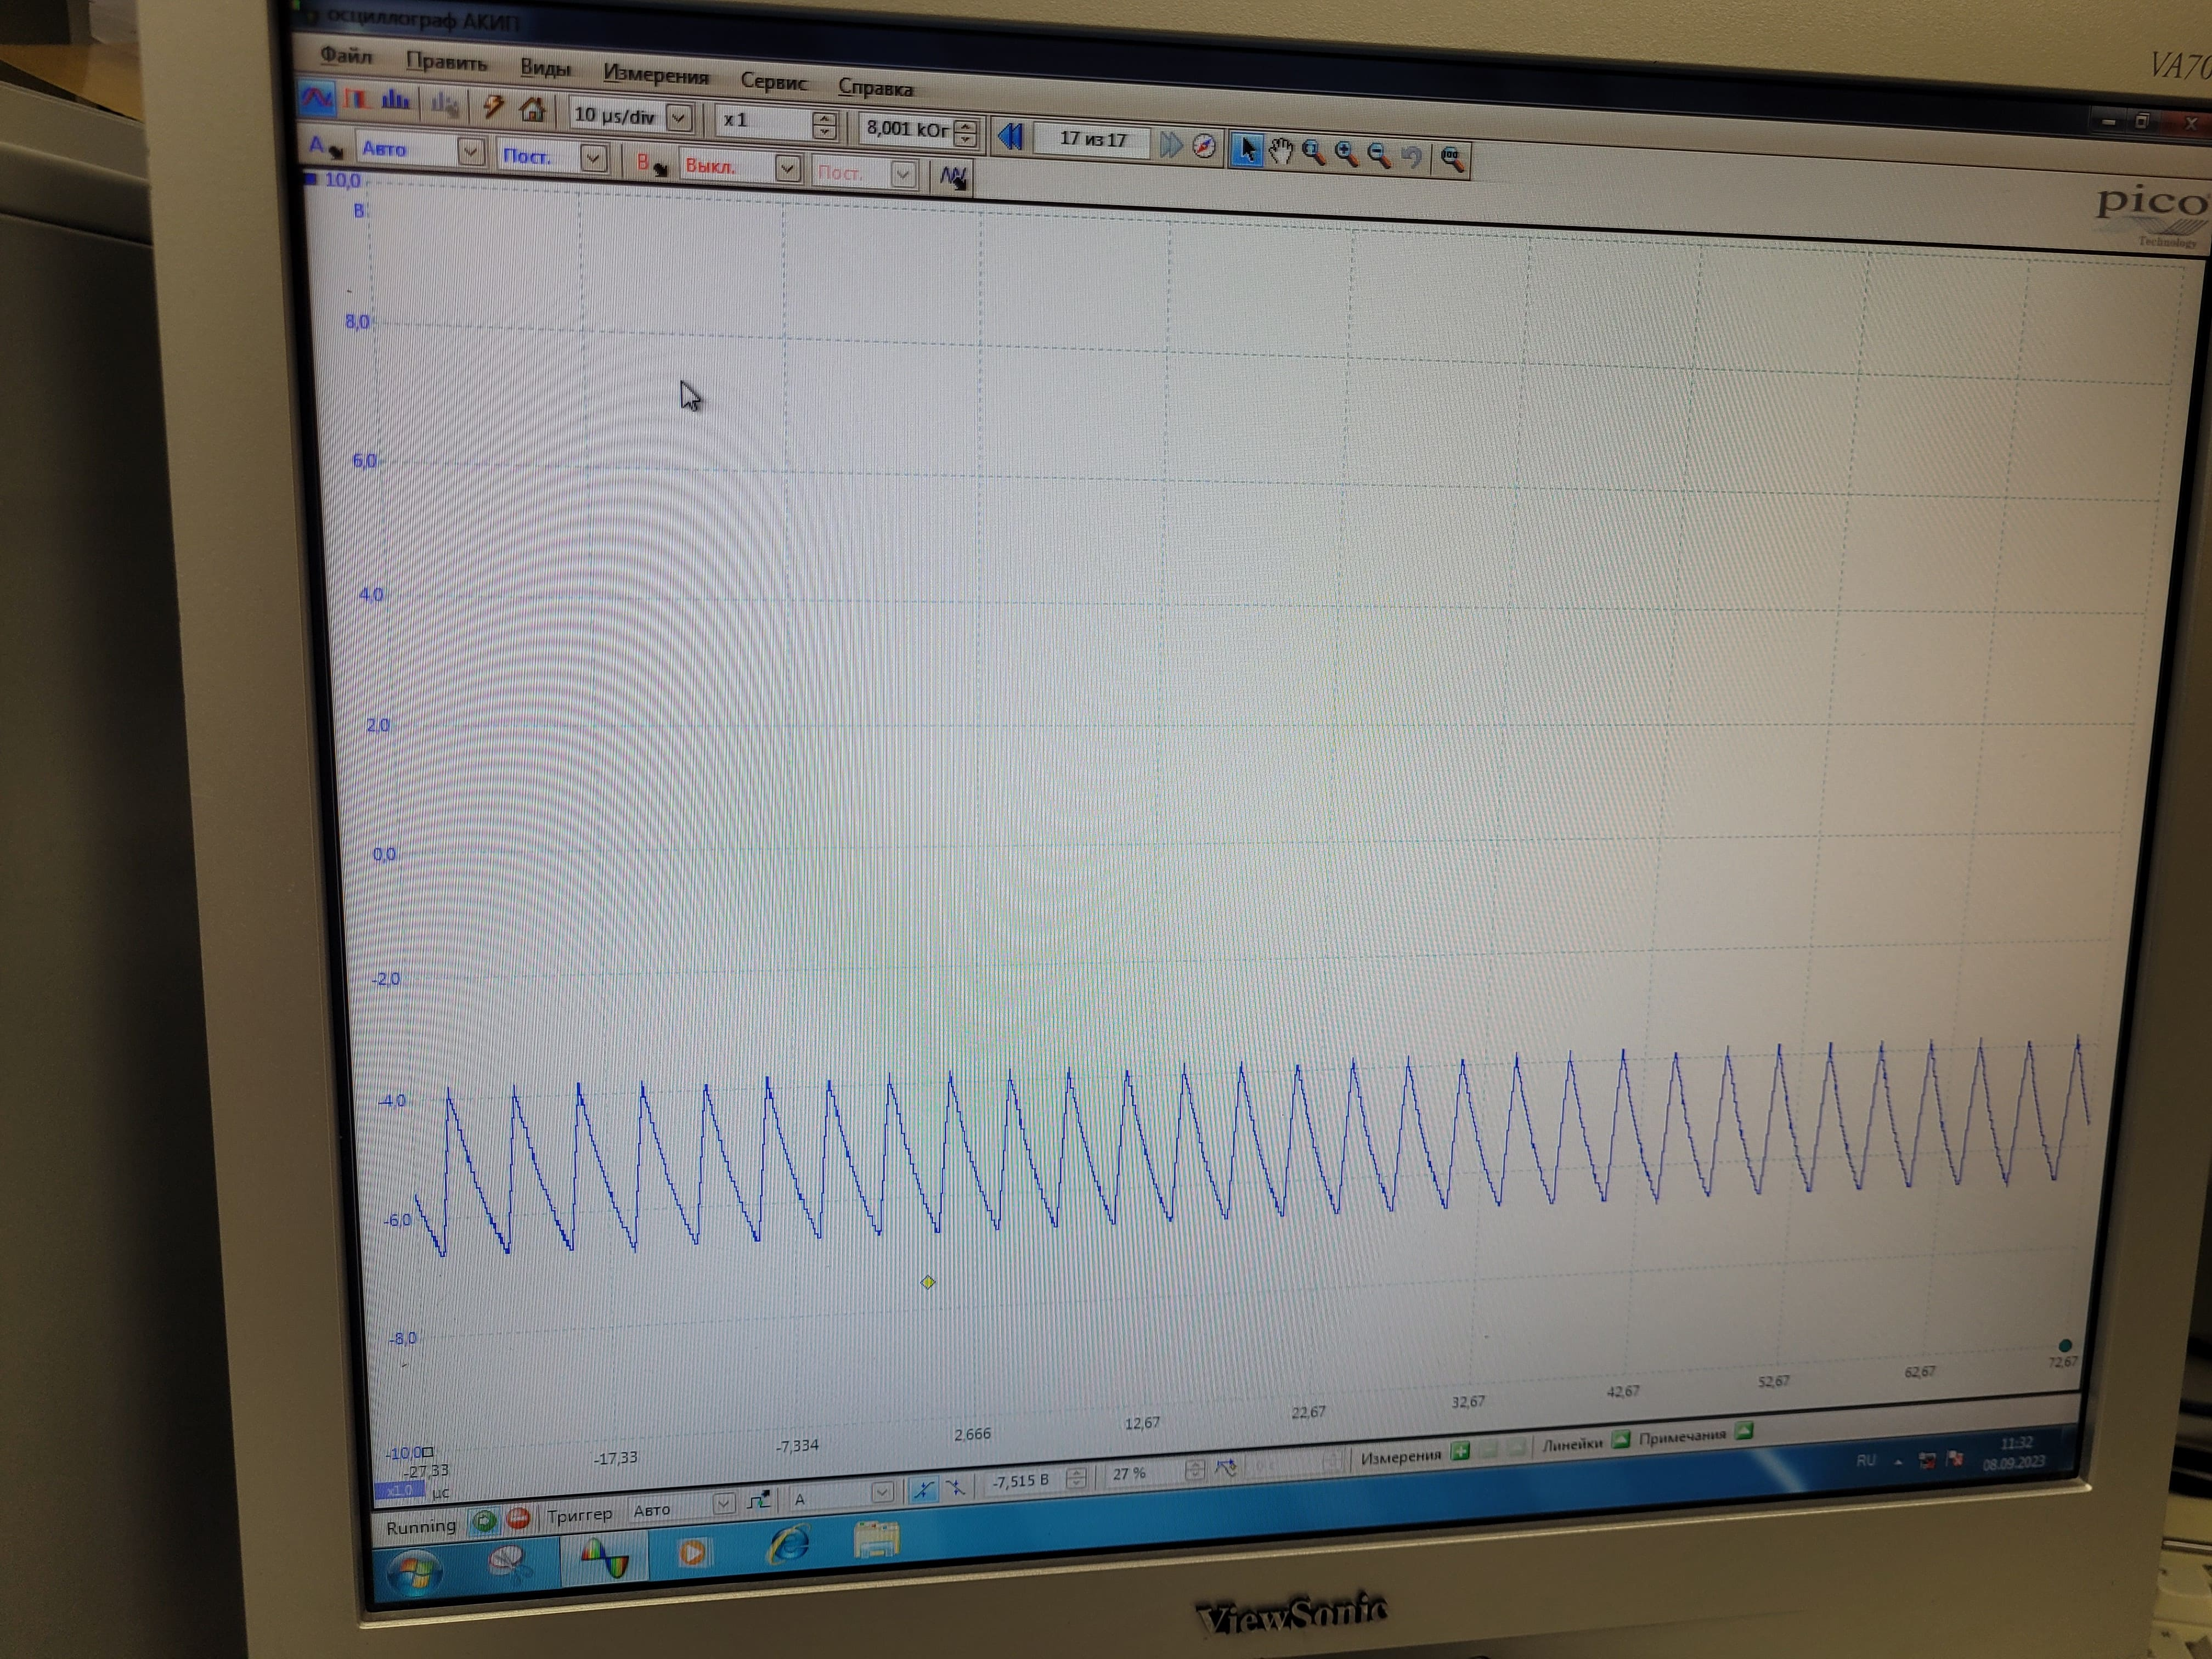
\includegraphics[width=1\linewidth]{E_sign_300k_510ns.jpg}} Сигнал при $\nu_0 = $ 300 кГц и $\tau$ = 510 нс.  \\
\end{minipage}
\hfill
\begin{minipage}[h]{0.44\linewidth}
\center{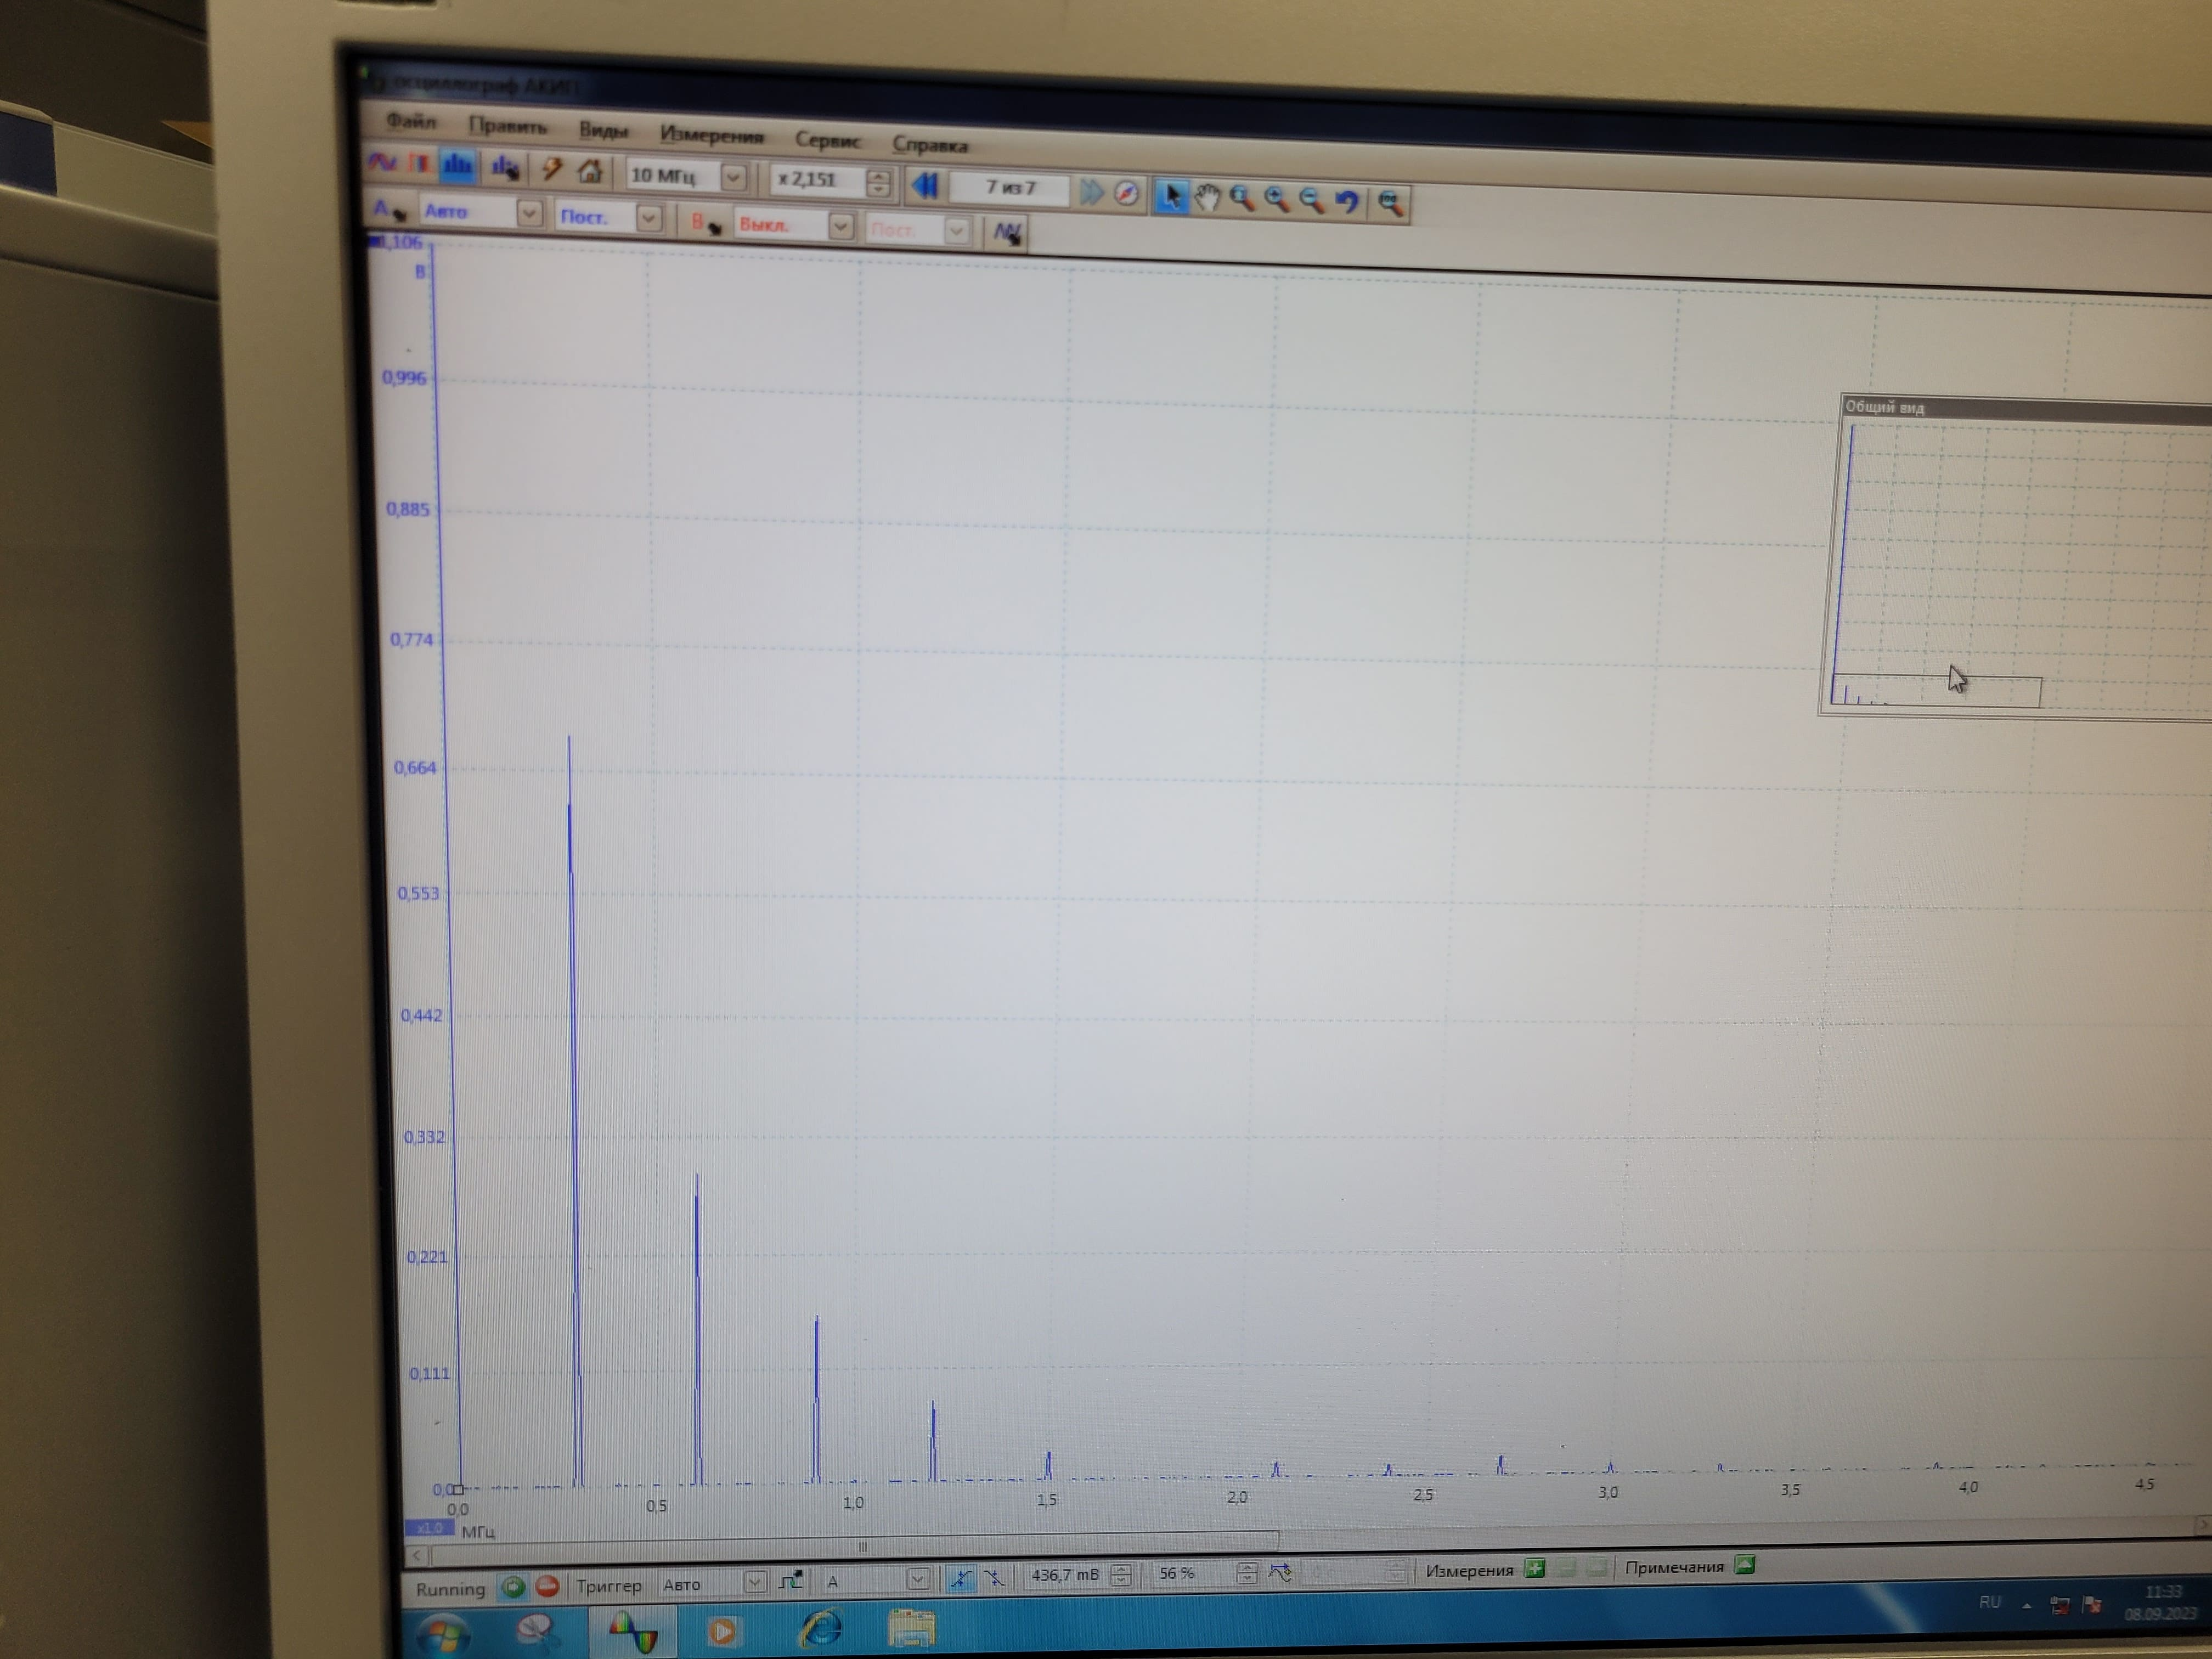
\includegraphics[width=1\linewidth]{E_spectr_300k_510ns.jpg}} \\  Спектр при $\nu_0 = $ 300 кГц и $\tau$ = 510 нс.
\end{minipage}
\vfill
\begin{minipage}[h]{0.44\linewidth}
\center{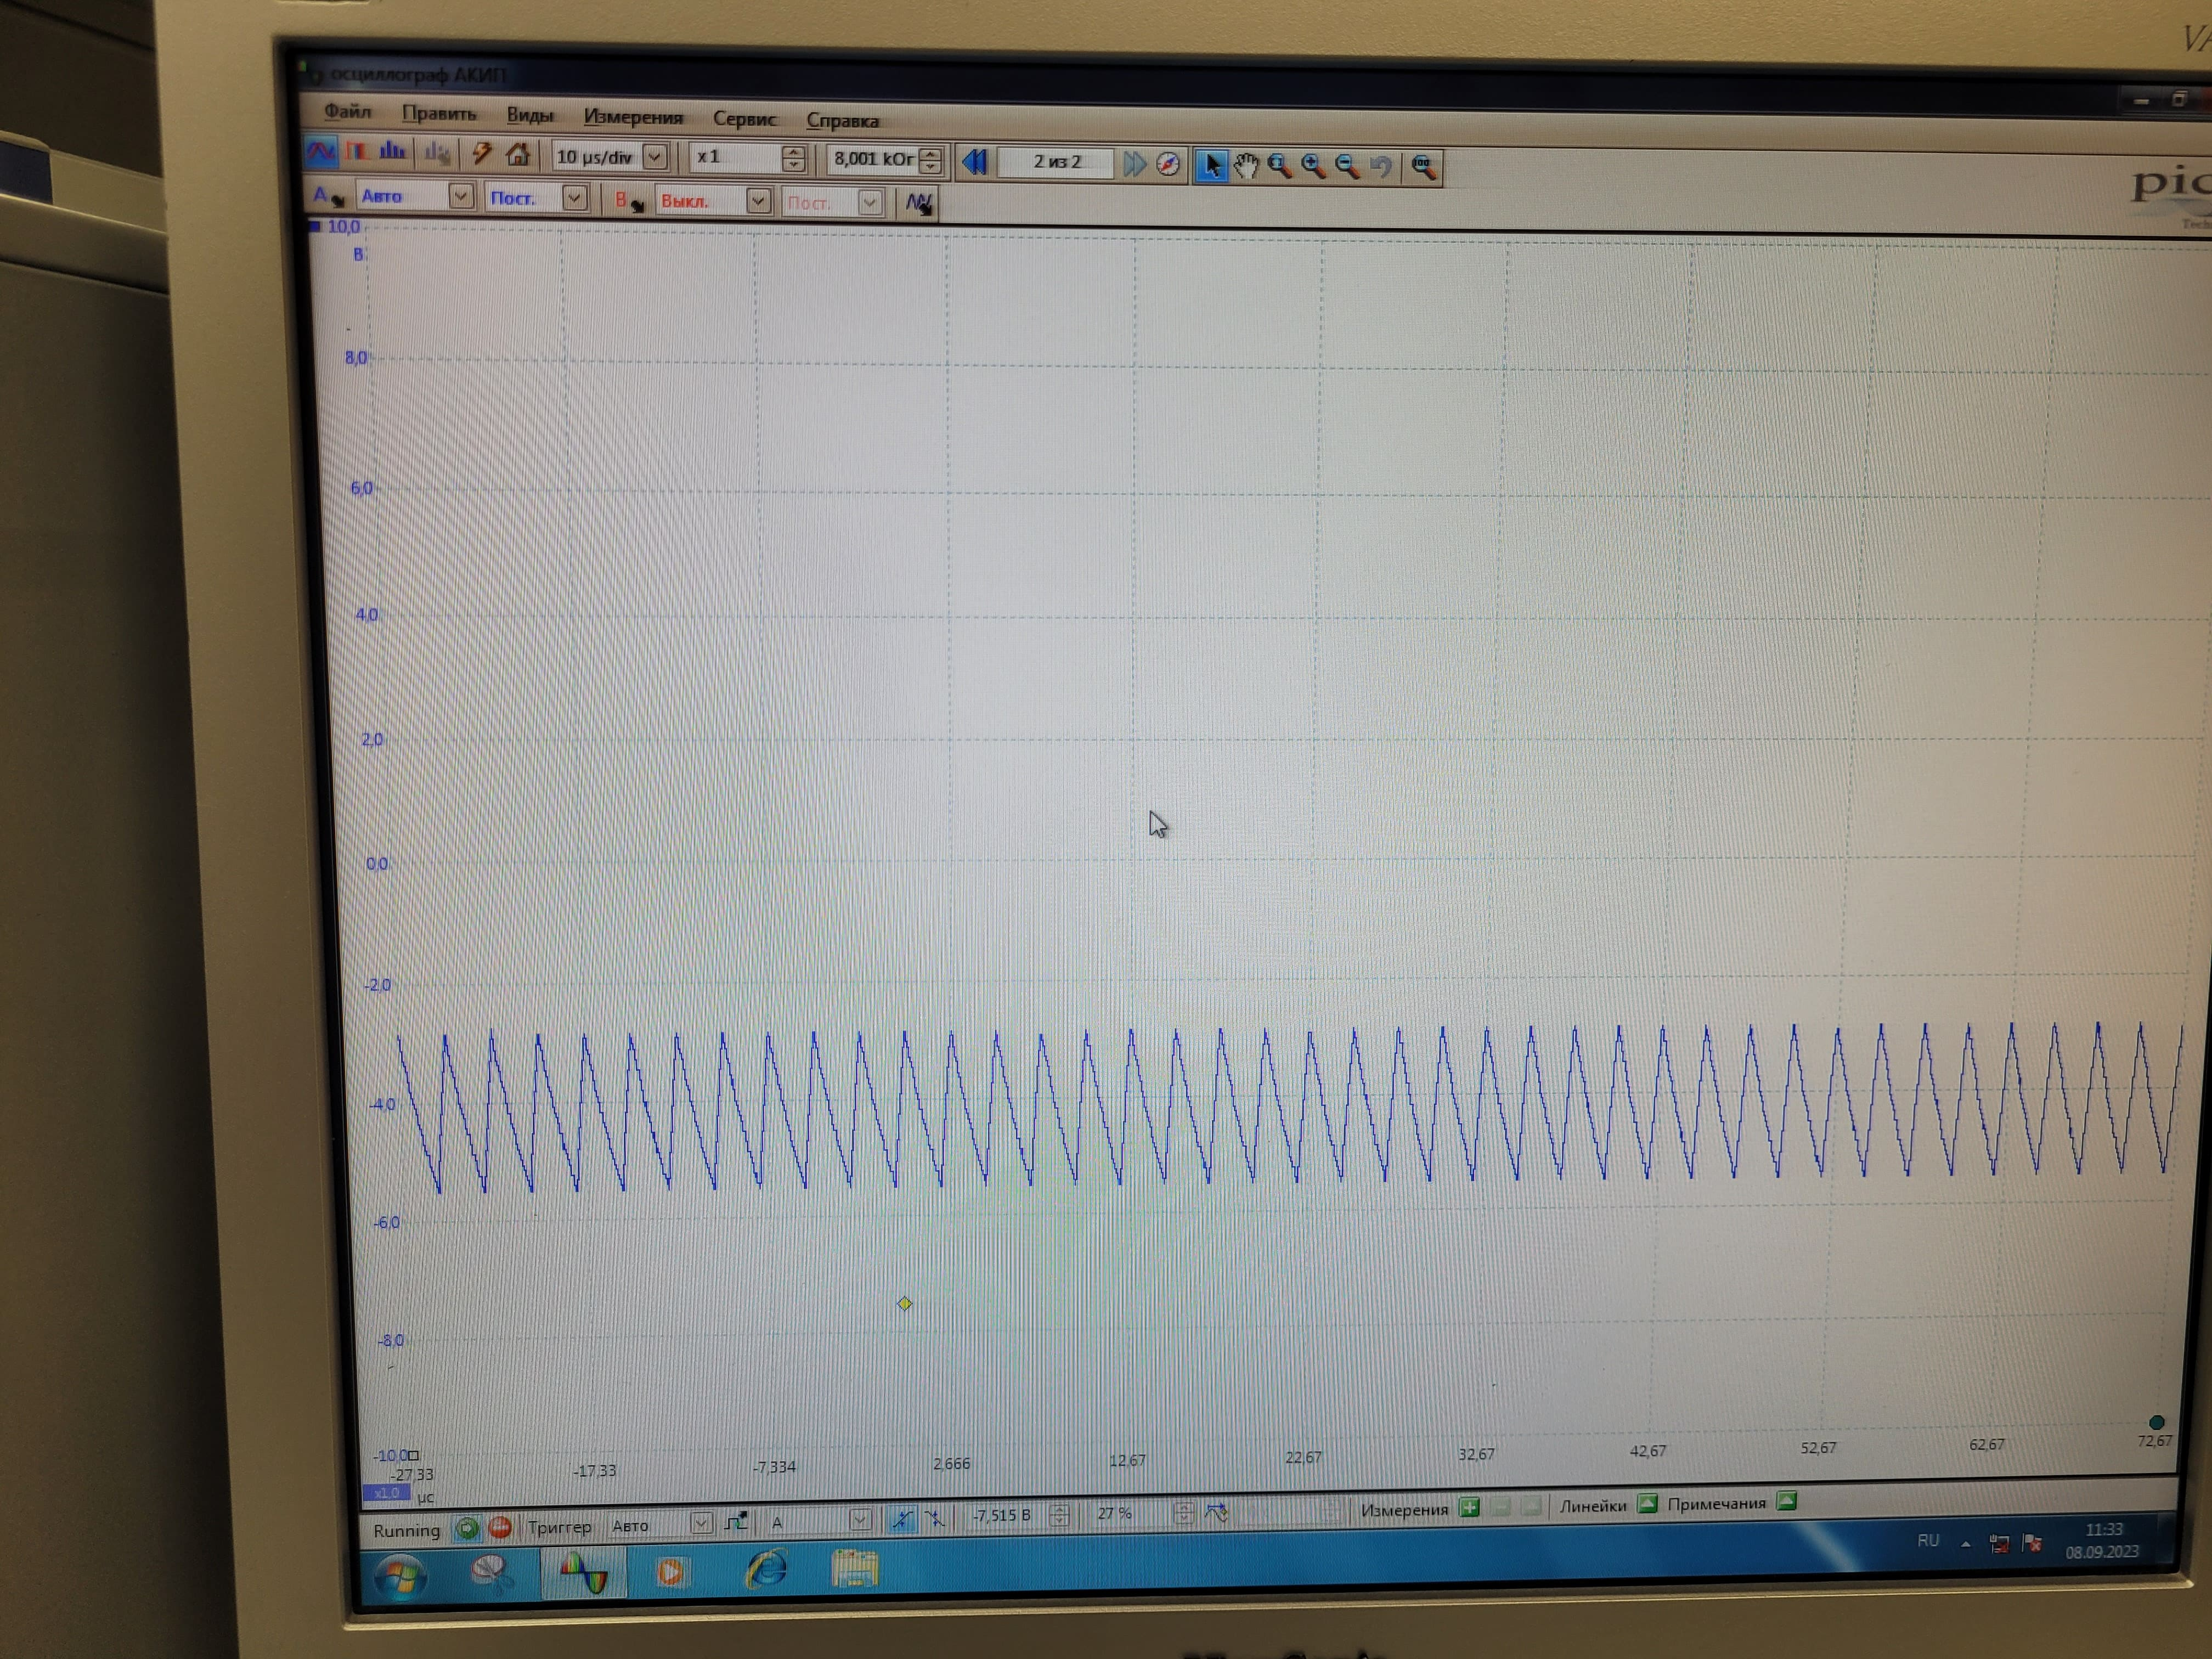
\includegraphics[width=1\linewidth]{E_sign_400k_510ns.jpg}} Сигнал при $\nu_0 = $ 400 кГц и $\tau$ = 510 нс.  \\
\end{minipage}
\hfill
\begin{minipage}[h]{0.44\linewidth}
\center{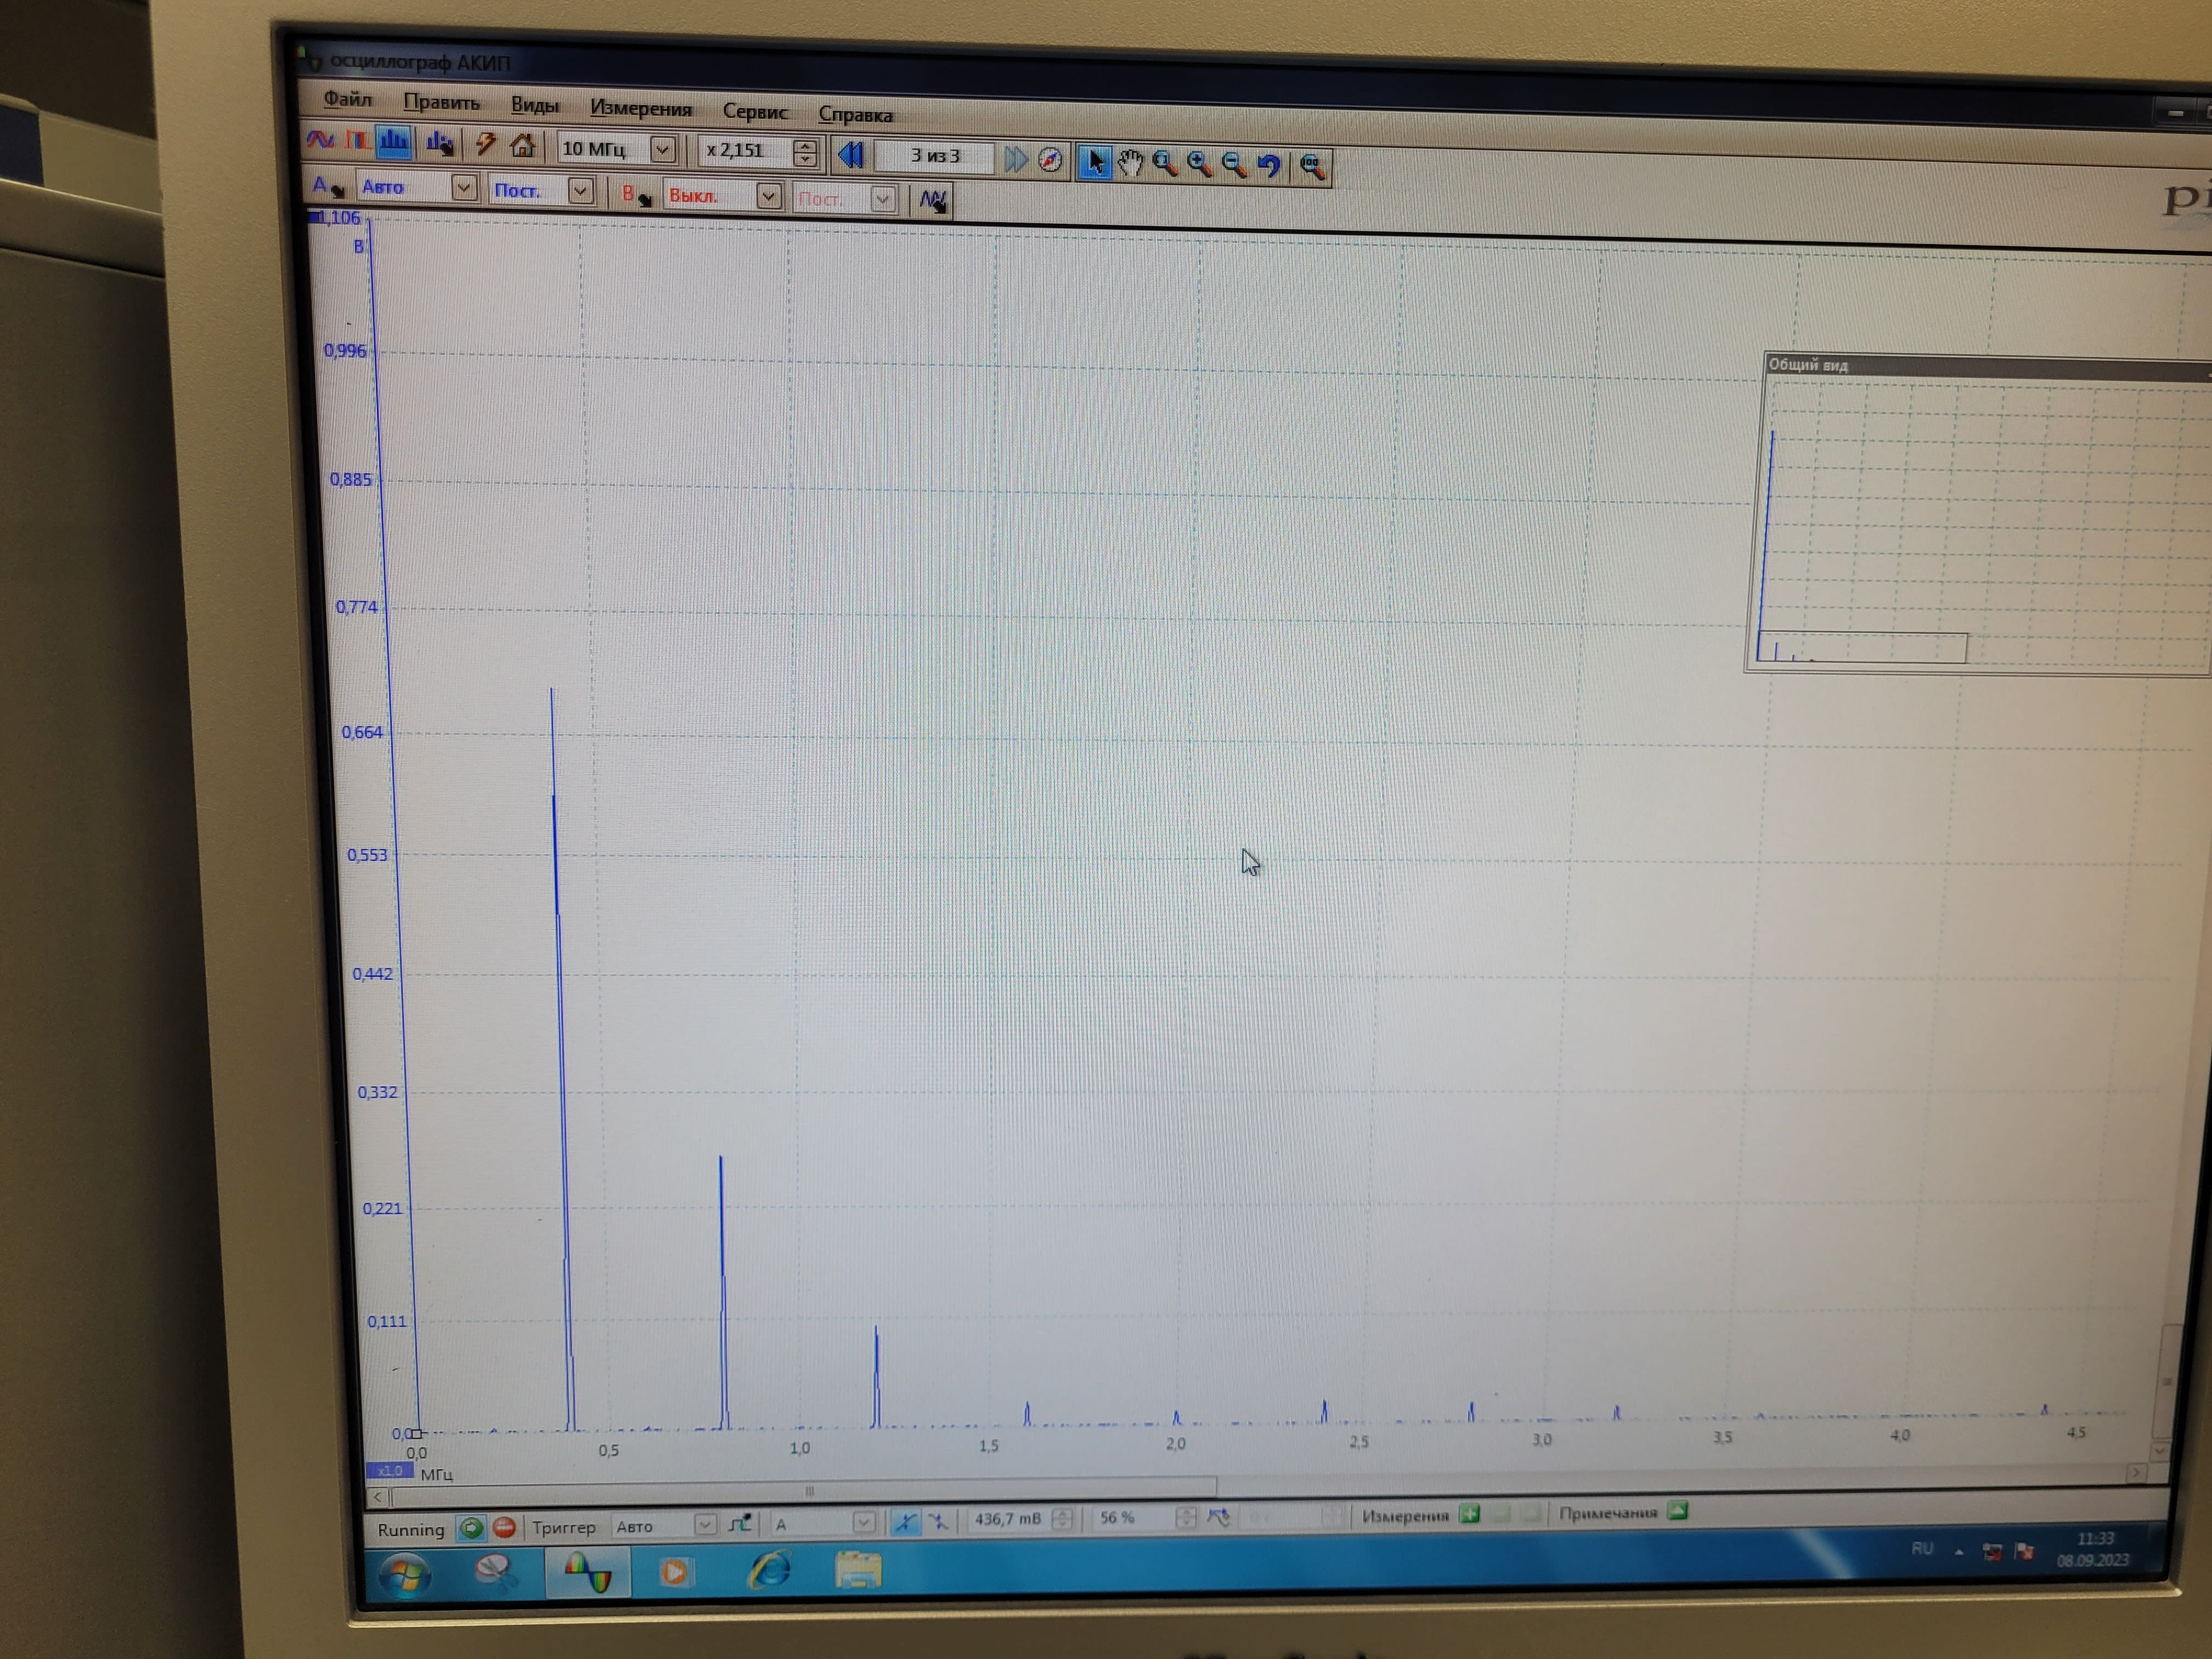
\includegraphics[width=1\linewidth]{E_spectr_400k_510ns.jpg}} Спектр при $\nu_0 = $ 400 кГц и $\tau$ = 510 нс. \\
\end{minipage}
\vfill
\caption{}
\label{ris:experimentalcorrelationsignals}
\end{figure}

\item [\textbf{3.}] 
При фиксированной частоте $\nu = 300$ кГц проведем измерения отношений амплитуд соответствующих спектральных гармоник (для 7–9 гармоник) фильтрованного и исходного сигналов: $K_n = |a_n^\text{ф}|/|a_n^0|$. Для измерения 
амплитуд $a_n^0$ спектра исходного сигнала переподключим генератор к осциллографу напрямую.

\begin{table}[h!]
    \centering
    \begin{tabular}{|c|c|c|c|c|c|c|c|c|c|}
\hline
$n$ & 1 & 2 & 3 & 4 & 5 & 6 & 7 & 8 & 9 \\ \hline
$a_n^\text{ф}$, мВ & 695.0 & 295.4 & 166.6 & 82.17 & 27.76 & 0 & 15.55 & 12.28 & 19.15 \\ \hline
$a_n^0$, мВ & 4452 & 3768 & 3151 & 1991 & 891 & 0 & 647 & 897 & 1008 \\ \hline
$K_n = |a_n^\text{ф}|/|a_n^0|$ & 0.156 & 0.078 & 0.0529 & 0.041 & 0.031 & ? & 0.024 &0.014 & 0.019 \\ \hline
\end{tabular}
    \caption{}
    \label{table4}
\end{table}

Построим график зависимости амплитудного коэффициента фильтрации $K(\nu)$ от частоты $\nu = n\nu_0$. 
\begin{figure}[h]
    \centering
    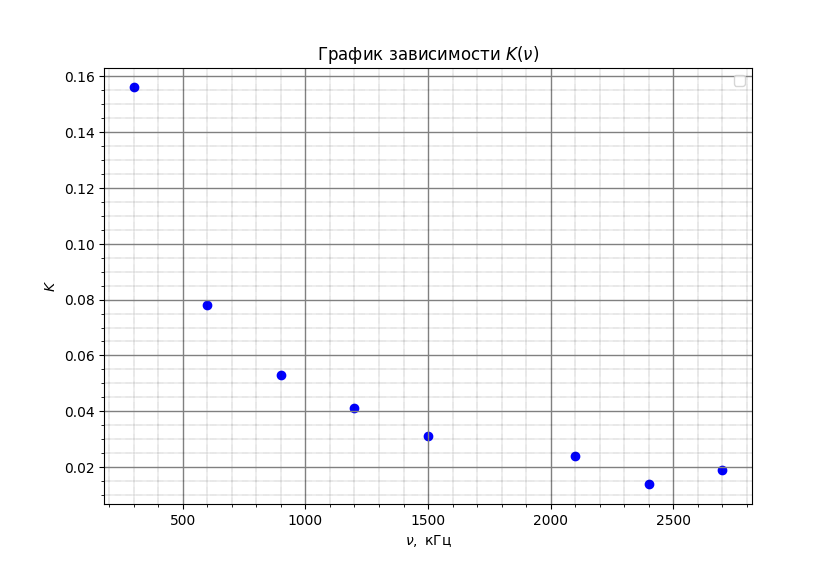
\includegraphics[width=0.7\linewidth]{K(nu).png}
    \caption{Зависимость $K(\nu)$}
    \label{grafic3}
\end{figure}





Проверим, что экспериментальная зависимость 
совпадает с теоретической $K = \frac{1}{\tau_\text{RC}} \int_0^t f(t')dt'$. Т.к. мы подаём последовательность прямоугольных импульсов, то права часть зависит линейно от $t$, т.е. обратно пропорционально $\nu$. График соответствует этой зависимости









\end{enumerate}



\newpage



\section{Обсуждение результатов и выводы}

В данной работе мы изучили понятие спектра и спектрального анализа, исследовали спектральный состав периодических электрических сигналов, а точнее прямоугольных импульсов, цугов гармонических колебаний, гауссиан, гармонических сигналов, модулированных по амплитуде и частоте, а также проанализировали фильтрацию сигналов при прохождении их через $RC$ контур. Проверили частный случай выполнения соотношения неопределённости.

\end{document}